%-----------------------------------------------------------------------
%   A Description of ogen - Overlapping Grid Generator
%
%-----------------------------------------------------------------------
\documentclass[xcolor=rgb,svgnames,dvipsnames]{article}
% \usepackage[bookmarks=true]{hyperref}
\usepackage[bookmarks=true,colorlinks=true,linkcolor=blue]{hyperref}

% \input documentationPageSize.tex
\hbadness=10000 
\sloppy \hfuzz=30pt

\usepackage{calc}
\usepackage[lmargin=.75in,rmargin=.75in,tmargin=.75in,bmargin=.75in]{geometry}

% \usepackage{calc}
% % set the page width and height for the paper (The covers will have their own size)
% \setlength{\textwidth}{7in}  
% \setlength{\textheight}{9.5in} 
% % here we automatically compute the offsets in order to centre the page
% \setlength{\oddsidemargin}{(\paperwidth-\textwidth)/2 - 1in}
% % \setlength{\topmargin}{(\paperheight-\textheight -\headheight-\headsep-\footskip)/2 - 1in + .8in }
% \setlength{\topmargin}{(\paperheight-\textheight -\headheight-\headsep-\footskip)/2 - 1in -.2in }


\input homeHenshaw

% \input pstricks
% \input pst-node

\usepackage{amsmath}
\usepackage{verbatim}
\usepackage{moreverb}
\usepackage{graphics}    
\usepackage{epsfig}    
\usepackage{multicol}
\usepackage{color}

% \usepackage{program}  % trouble with pdflatex

% -- new way: todo: 
% \usepackage{listings}
% \lstset{
% basicstyle=\footnotesize\ttfamily,
% columns=flexible,
% breaklines=true,
% commentstyle=\color{red},
% keywordstyle=\color{black}\bfseries
% }

\usepackage{makeidx} % index
\makeindex
\newcommand{\Index}[1]{#1\index{#1}}


\usepackage{tikz}
\input trimFig.tex

% \usepackage{float}

% \input colours.tex

% ---- we have lemmas and theorems in this paper ----
% ---- we have lemmas and theorems in this paper ----
\newtheorem{assumption}{Assumption}
\newtheorem{definition}{Definition}

\input wdhDefinitions

\newcommand{\MGF}{Mapped\-Grid\-Function}
\newcommand{\GCF}{Grid\-Collection\-Function}
\newcommand{\CGF}{Composite\-Grid\-Function}

\newcommand{\MGO}{Mapped\-Grid\-Operators}
\newcommand{\GCO}{Grid\-Collection\-Operators}
\newcommand{\CGO}{Composite\-Grid\-Operators}

\newcommand{\primer}{Overture/primer}
\newcommand{\sampleGrids}{Overture/sampleGrids}

% Put figures in cgDoc/fig
\newcommand{\figures}{../fig}
%\newcommand{\figures}{\homeHenshaw/OvertureFigures}

\newcommand{\mapping}{\OvertureDir/mapping}

\newcommand{\ogshow}{\OvertureDir/ogshow}
\newcommand{\ogen}{\OvertureDir/ogen}
% \newcommand{\cguser}{\homeHenshaw/cgap/cguser}


% *** See http://www.eng.cam.ac.uk/help/tpl/textprocessing/squeeze.html
% By default, LaTeX doesn't like to fill more than 0.7 of a text page with tables and graphics, nor does it like too many figures per page. This behaviour can be changed by placing lines like the following before \begin{document}

\renewcommand\floatpagefraction{.99}
\renewcommand\topfraction{.99}
\renewcommand\bottomfraction{.99}
\renewcommand\textfraction{.1}   
\setcounter{totalnumber}{50}
\setcounter{topnumber}{50}
\setcounter{bottomnumber}{50}


% ========================================================================================================================
% ========================================================================================================================
% ========================================================================================================================
\begin{document}



%---------- Title Page for a Research Report----------------------------
\vglue5\baselineskip
\index{grid generation}
\begin{flushleft}
{\Large
Ogen: An Overlapping Grid Generator for Overture \\
}
\vspace{2\baselineskip}
William D. Henshaw  \\
Department of Mathematical Sciences, \\
Rensselaer Polytechnic Institute, \\
Troy, NY, USA, 12180. \\
\vspace{2\baselineskip}
\today 
% William D. Henshaw
% \footnote{
%         This work was partially
%         supported by grant N00014-95-F-0067 from the Office of Naval
%         Research}  \\
% CASC: Centre for Applied Scientific Computing\footnote{Management prefers the spelling `Center'}  \\
% Lawrence Livermore National Laboratory    \\
% Livermore, CA, 94551   \\
% henshaw@llnl.gov \\
% http://www.llnl.gov/casc/people/henshaw \\
% http://www.llnl.gov/casc/Overture  \\
% \vspace{\baselineskip}
% UCRL-MA-132237
% LA-UR-96-3466

\vspace{4\baselineskip}

\noindent{\bf Abstract:}

% {\bf NOTE: This grid generator is new and will only appear with Overture.v14 }

We describe how to generate overlapping grids for use with Overture using the
{\tt ogen} program. The user must first generate {\tt Mappings} to describe the
geometry (a set of overlapping grids whose union covers the domain). The overlapping
grid then is constructed using the {\tt Ogen} grid generator. This latter step consists
of determining how the different component grids interpolate from each other, and in
removing grid points from holes in the domain, and removing unnecessary grid points 
in regions of excess overlap. This document includes a description of commands, presents
a series of command files for generating various overlapping grids and describes the
overlapping grid algorithm. The {\tt ogen} program can also be used to build unstructured
hybrid grids where the overlap is replaced by an unstructured grid.
\end{flushleft}

\clearpage
\tableofcontents

\clearpage

% ----------------------------------------------------------------------------------------
\section{Introduction}

The ogen program can be used to interactively generate overlapping grids. 


The basic steps to follow when creating an overlapping grid are
\begin{itemize}
  \item create mappings that cover a domain and overlap where they meet.
  \item generate the overlapping grid (ogen calls the grid generator Ogen).
  \item save the grid in a data-base file.
\end{itemize}

The {\tt ogen} program is found in the {\tt Overture/bin} directory. Just type
{\tt ogen} to get started. You can also type {\tt `ogen noplot'} in which case
{\tt ogen} will run without graphics. This is useful if you just want to 
execute a command file to regenerate a grid -- running without graphics
is faster. If you have a command file, {\tt example.cmd}, then you can type {\tt `ogen example.cmd'}
or {\tt `ogen example'} (a {\tt .cmd} will automatically be added) to run the commands in the file. 
To run without graphics type {\tt `ogen noplot example'}.

Once you have made a grid and saved it in a data-base file 
(named {\tt myGrid.hdf}, for example) you can
look at it using the command {\tt Overture/\-bin/\-plotStuff myGrid.hdf} 
(or just {\tt Overture/\-bin/\-plotStuff myGrid}). 

Figure \ref{fig:ogen} shows a snap-shot of {\tt ogen} running.
% \begin{figure}[htb]
%   \begin{center}
%    \epsfig{file=\figures /ogenScreenSub.ps,width=\linewidth} % .7
%   \caption{A snapshot of ogen}  \label{fig:ogen}
%   \end{center}
% \end{figure}
{
\newcommand{\figWidthd}{9cm}
\newcommand{\trimfig}[2]{\trimPlot{#1}{#2}{.0}{.0}{.0}{.0}}
\begin{figure}[hbt]
\begin{center}
\begin{tikzpicture}[scale=1]
  \useasboundingbox (0,.5) rectangle (9.,8.5);  % set the bounding box (so we have less surrounding white space)
%
  \draw ( 0.0,0.) node[anchor=south west,xshift=-4pt,yshift=+0pt] {\trimfig{\figures/ogenScreenSub}{\figWidthd}};
%
 % \draw (current bounding box.south west) rectangle (current bounding box.north east);
% grid:
% \draw[step=1cm,gray] (0,0) grid (9,8);
\end{tikzpicture}
\end{center}
\caption{A snapshot of ogen} \label{fig:ogen}
\end{figure}
}

\noindent
Other documents of interest that are available through the Overture home page are
\begin{itemize}
\item Mapping class documentation : {\tt mapping.tex}, \cite{MAPPINGS}. Many of the mappings that
   are used to create an overlapping grid are documented here. 
\item Interactive plotting : {\tt PlotStuff.tex}, \cite{PLOTSTUFF}.
\end{itemize}


% -------------------------------------------------------------------------------------------------
\section{Commands}

\subsection{Commands for ogen}

The commands in the initial {\tt ogen} menu  are
\begin{description}
  \item[create mappings] : create mappings to represent the geometry. See section (\ref{sec:createMappings}).
  \item[generate an overlapping grid] : once mappings have been created an overlapping grid
    can be generated with this option. This will call the Ogen grid generator. See section 
       (\ref{sec:ogen:commands}) for a list of the commands available with the grid generator.
  \item[make an overlapping grid] : this calls the old Cgsh grid generator, the original Overture
     grid generator.
  \item[save and overlapping grid] : Save an overlapping grid in a data base file.
\end{description}

\subsection{Commands when creating Mappings} \label{sec:createMappings}

The basic commands available from the {\tt create mappings} menu option are (this list will in general
be out of date so you are advised to run {\tt ogen} to see the currently available options). 
Most of these commands simply create a new Mapping and call the update function for that Mapping.
Descriptions of the {\bf Mapping's} referred to here can be found in the mapping documentation
\cite{MAPPINGS}.

\begin{description}
  \item[help] : output minimal help.
  \item[1D Mappings] :
  \begin{description}
    \item[line] : Build a line in 1D. This can be used for a 1D overlapping grid. Reference {\tt LineMapping}.
    \item[stretching function] : Reference {\tt StretchMapping}.
    \item[spline (1D)] : Reference {\tt SplineMapping}.
  \end{description}
  \item[2D Mappings] :
  \begin{description}
    \item[Airfoil] : Build a two-dimensional airfoil from various choices including the NACA 4 digit series
      airfoils.  Reference {\tt AirfoilMapping}.
    \item[Annulus] :  Reference {\tt AnnulusMapping}.
    \item[Circle or ellipse] :  Reference {\tt CircleMapping}.
    \item[DataPointMapping] : Build a new Mapping from a set of discrete data points.
        The data points may be read from a plot3d file. Reference {\tt DataPointMapping}.
    \item[line (2D)] : Reference {\tt LineMapping}.
    \item[nurbs (curve)] : build a NURBS (a type of spline) curve or surface from control points or by
      interpolating data points.  Reference {\tt NurbsMapping}.
    \item[rectangle] :  Reference {\tt SquareMapping}. 
    \item[SmoothedPolygon] : Build a grid or curve with a boundary that is a polygon with
        smoothed out corners. Reference {\tt SmoothedPolygonMapping}. 
    \item[spline] : Reference {\tt SplineMapping}.
    \item[tfi] :  Build a new Mapping from existing curves or surfaces using 
          transfinite interpolation (Coon's patch). Reference {\tt TFIMapping}.
  \end{description}
  \item[3D Mappings] :
  \begin{description}
    \item[Box] : Reference {\tt BoxMapping}. 
    \item[Cylinder] :  Reference {\tt CylinderMapping}. 
    \item[Circle or ellipse (3D)] :  Reference {\tt CircleMapping}.
    \item[CrossSection] : Reference {\tt CrossSectionMapping}.
    \item[DataPointMapping] : Build a new Mapping from a set of discrete data points.
        The data points may be read from a plot3d file. Reference {\tt DataPointMapping}.
    \item[line (3D)] : Reference {\tt LineMapping}.
    \item[nurbs (surface)] :build a NURBS (a type of spline) curve or surface from control points or by
      interpolating data points.  Reference {\tt NurbsMapping}.
    \item[plane or rhombus] : Reference {\tt PlaneMapping}.
    \item[Sphere] : Reference {\tt SphereMapping}.
    \item[spline (3D)] : Reference {\tt SplineMapping}.
    \item[tfi] : Build a new Mapping from existing curves or surfaces using 
          transfinite interpolation (Coon's patch). Reference {\tt TFIMapping}.
  \end{description}
  \item[transform] :
  \begin{description}
    \item[body of revolution] : create a body of revolution from a two-dimensional
       Mapping. Reference {\tt Revolution\-Mapping}. 
    \item[elliptic] : generate an elliptic grid on an existing grid in order to redistribute
        grid points. Reference {\tt Elliptic\-Transform}. 
    \item[fillet] : Build a fillet surface to join two intersecting surfaces. Reference {\tt Fillet\-Mapping}. 
    \item[hyperbolic] : Reference {\tt Hyperbolic\-Mapping}.
    \item[hyperbolic surface] :  Reference {\tt Hyperbolic\-Surface\-Mapping}.
    \item[intersection] : Determine the intersection curve between two intersecting surfaces. 
            Reference {\tt Intersection\-Mapping}.
    \item[mapping from normals] :  Generate a new Mapping by extending normals from a curve or a surface.
         Reference {\tt NormalMapping}.
    \item[reparameterize] :  reparameterize an existing Mapping by 
      \begin{enumerate}
       \item restricting the domain space to a sub-rectangle (this would be used to create an refinement patch 
         on an adaptuve grid) 
       \item remove a polar singularity by creating a new patch with an orthographic transform.
      \end{enumerate}
        Reference {\tt Reparameterization\-Transform}, {\tt Orthographic\-Transform} and
                      {\tt Restriction\-Mapping}.
    \item[rotate/scale/shift] : transform an existing Mapping. Reference {\tt MatrixMapping}.
    \item[stretch coordinates] : stretch (cluster) the grid points in the coordinate directions.
         Reference {\tt Stretch\-Transform} and {\tt Stretch\-Mapping}. 
  \end{description}
  \item[change] :
  \begin{description}
    \item[change a mapping] : Make changes to an existing Mapping.
    \item[copy a mapping] : Make a copy of an existing Mapping.
    \item[delete a mapping] : delete an existing Mapping.
  \end{description}
  \item[data base] :
  \begin{description}
    \item[open a data-base] : open an Overture data-base file (new or old).
    \item[get from the data-base] : read Mapping's from the data-base.
    \item[put to the data-base] : save a Mapping in the data-base.
    \item[close the data-base] : close the data-base.
    \item[save plot3d file] : write a plot3d file.
  \end{description}
   \item[read from file] :
  \begin{description}
    \item[read plot3d file] : read a plot3d formatted file and extract the grids. Each grid becomes a
         {\tt DataPointMapping}.
    \item[read iges file] : *experimental* read an IGES (Initial Graphics Exchange Specification) file
        such as created by pro/ENGINEER and build NURBS and trimmed NURBS found in the file.
    \item[read overlapping grid file] : read an existing overlapping grid data base file and extract all
      the Mapping's from it. These Mappings can then be changed.
  \end{description}
  \item[view mappings] : view the currently defined Mappings.
  \item[check mapping] : check a Mapping to see that it is defined properly. This is normally only done
     when one defines a new Mapping.
  \item[exit this menu] :
\end{description}




\section{Things you should know to make an overlapping grid}


Here are some things that you will need to know when building overlapping grids. 
The examples that follow will demonstrate all of these ideas.

\input overlappingGridCartoon

Figure~\ref{fig:overlappingGridCartoon} illustrates a simple two-dimensional overlapping grid. The computational
domain is covered with two component grids $\xv=G_1(\rv)$ and $\xv=G_2(\rv)$. 
% In order to properly define the domain we need to specify {\em boundary conditions}. These indicate which 




\subsection{Boundary conditions}\label{sec:bc}

   Each side of each component grid must be given a boundary condition value. These
boundary conditions are essential since they indicate whether a boundary is a 
physical boundary\index{boundary condition!physical boundary}
 (a value greater than 0), an interpolation boundary (a value equal
to zero) or a side that is has a periodic boundary condition (a value less than zero). 
The \Index{boundary condition} values are stored in an array as
\begin{align*}
{\tt boundaryCondition}({\tt side},{\tt axis}) 
    &= \begin{cases}
        > 0 & \text{physical boundary} \\
        =0  & \text{interpolation boundary} \\
        < 0 & \text{periodic boundary} 
      \end{cases} \\
 {\tt boundaryCondition}(0,0) &= \text{left} \\ 
 {\tt boundaryCondition}(1,0) &= \text{right} \\ 
 {\tt boundaryCondition}(0,1) &= \text{bottom} \\ 
 {\tt boundaryCondition}(1,1) &= \text{top} \\ 
 {\tt boundaryCondition}(0,2) &= \text{front (3D)} \\ 
 {\tt boundaryCondition}(1,2) &= \text{back (3D)} 
\end{align*}
where {\tt side=0,1} and {\tt axis=0,1} in 2D, or {\tt axis=0,1,2} in 3D, indicates the face of the the grid.
Note that each grid is a mapping from the unit square or unit cube to a physical domain -- the terms left, right,
bottom, top, front and back refer to the sides of the unit square or cube.
When you enter the boundary condition values (when changing them in a mapping) you should enter
them in the order: left, right, bottom, top, front, back. 
   
The grid generator uses physical boundaries to cut holes in other grids that happen to cross that
physical boundary. See, for example, the ``cylinder in a channel example'' where the rectangular 
grid has a hole cut out of it.  Interpolation boundaries are non-physical boundaries where the
grid generator will attempt to interpolate the points from other component grids. A periodic boundary
can be either be a branch cut (as on an annulus) or it can indicate a periodic domain (as with a
square where the right edge of the square is to be identified with the left edge).


% If you incorrectly specify a boundary to be a physical boundary when it i


\subsection{Share flag}\label{sec:share}

The \Index{share flag} is used to indicate when two different component grids share a common boundary (see
the ``inlet outlet'' example, section (\ref{sec:inletOutlet}). 
The grid generator uses the share flag so that a boundary of one
component grid will not accidently cut a hole in another grid when the two grids are actually part
of the same boundary. This could happen since, due to inaccuracies in representing each grid, it
may seem that the boundary on one grid lies inside or outside the other grid (even though they
are meant to be the same boundary curve).

The share flag is saved in an array that is the same shape as the {\tt boundary condition} array
\begin{align*}
{\tt share}({\tt side},{\tt axis}) 
            &> 0   \quad\text{a code that should be the same on all shared boundaries.} \\
 {\tt share}(0,0) &= \text{left} \\ 
 {\tt share}(1,0) &= \text{right} \\ 
 {\tt share}(0,1) &= \text{bottom} \\ 
 {\tt share}(1,1) &= \text{top} \\ 
 {\tt share}(0,2) &= \text{front (3D)} \\ 
 {\tt share}(1,2) &= \text{back (3D)} 
\end{align*}
where {\tt side=0,1} and {\tt axis=0,1} in 2D, or {\tt axis=0,1,2} in 3D, indicates the face of the the grid.

Thus the share flags on all grid faces that belong to the same boundary should be
given the same share value. This could be accomplished by setting all {\tt share} values to $1$ say,
although this is slightly dangerous as the grid generator could make a mistake. It is better
to use a different positive integer for each different boundary.


\subsection{Turning off the cutting of holes}\label{sec:cuttingHoles}\index{cutting holes!turning off}

  By default, the overlapping grid generator will use any  physical boundary (a side of a grid
with a positive {\tt boundaryCondition} to try and cut holes in any other grid that lies near
the physical boundary. Thus in the ``cylinder in a channel example'' section (\ref{sec:cylinderInAChannel})
the inner boundary of the annulus cuts a hole in the rectangular grid. 
Sometimes, as in the ``inlet outlet'' example, section (\ref{sec:inletOutlet}),
one does not want this to happen. In this case it is necessary to explicitly specify which
grids are allowed to cut holes in which other grids. This can be done through in the 
{\tt change parameters} option with the {\tt prevent hole cutting} option, see
section the ``inlet outlet'' example, (\ref{sec:inletOutlet}).


\subsection{Turning off interpolation between grids}\label{sec:turningOffInterpolate}\index{interpolation!turning off}

  By default all grids can interpolate from all other grids. This default can be changed and you may specify
which grids may interpolate from which other grids. This option can be used, for example, to build 
grids for two disjoint domains that match along a boundary as shown in figure~(\ref{fig:innerOuter}).



\subsection{Implicit versus explicit interpolation} \label{sec:interpolation}

   There are two types of \Index{interpolation}, {\bf explicit}\index{interpolation!explicit}
 and {\bf implicit}\index{interpolation!implicit}.
{\bf Explicit} interpolation means that a point that
is interpolated will only use values on other grids that are not interpolation points themselves. 
This means that will the default 3 point interpolation the amount of overlap must be at least
$1.5$ grid cells wide. With explicit interpolation the interpolation equations can be solved 
explicitly (and this faster).

With {\bf implicit} interpolation the points used in the interpolation
stencil may themselves be interpolation points. This means  
that will the default 3 point interpolation the amount of overlap must be at least
$.5$ grid cells wide. Thus {\bf implicit interpolation is more likely to give a valid grid} since
it requires less overlap. With implicit interpolation the interpolation equations are a coupled
system that must be solved. This is a bit slower but the Overture interpolation function handles
this automatically.



\clearpage
% =================================== EXAMPLES ==============================================================
\section{Examples}

In this section we describe a number of {\sl command files}\index{command file} that can be used to
create various overlapping grids. During an interactive session a command file
can be saved, see the option {\tt `log commands to file'} in the {\tt file} pull-down menu. 
By default the command file {\tt ogen.cmd} is automatically saved.
The command file will record all the commands that are issued. The command file
can be later read in, using {\tt `read command file'} in the {\tt file} pull-down menu,
and the commands will be executed. You can also type {\tt `ogen example.cmd'} to run the command file
named {\tt example.cmd} with graphics or {\tt `ogen noplot example.cmd'} to run without graphics.

The command file can be edited and changed. Once a complicated grid has been created
it is usually easiest to make minor changes by editing the command file. The {\tt pause}
command can be added to the command file which will cause the program to pause at that
point and wait for an interactive response -- one can then can either {\tt continue} or {\tt break}.


% --------------------------------------------------------------------------------------------------------
\subsection{Square}

Here is a command file to create a square.
(file {\tt \sampleGrids/square5.cmd})
We first  make a mapping for the square and assign various parameters such as
the number of grid points
and the boundary conditions. Any positive number for the boundary condition indicates
a physical boundary. 
Next the overlapping grid generator is
called ({\tt make an overlapping grid}) to make an overlapping grid (which
is trivial in this case). Finally the overlapping grid is saved in a data-base file.
The data-base file is an HDF formatted file.
HDF is the the Hierarchical Data Format (HDF) from the National Centre
for Super-Computing Applications (NCSA). You can look at the data base file created here 
by typing {\tt plotStuff square5.hdf} (or just {\tt plotStuff square5})
where {\tt plotStuff} is found in {\tt Overture/bin}.
% The resulting grid is shown in figure~\ref{fig:square}.

% \noindent
\begin{minipage}{.4\linewidth}
{\footnotesize
% new way: todo:
% \lstinputlisting[language=Matlab, numbers=left, stepnumber=1, firstline=1,caption={square5.cmd},label=cmd:square5,frame=single]{\ogen/square5.cmd}
\listinginput[1]{1}{\ogen/square5.cmd}
}
\end{minipage}\hfill
\begin{minipage}{.6\linewidth}
  \begin{center}
   % 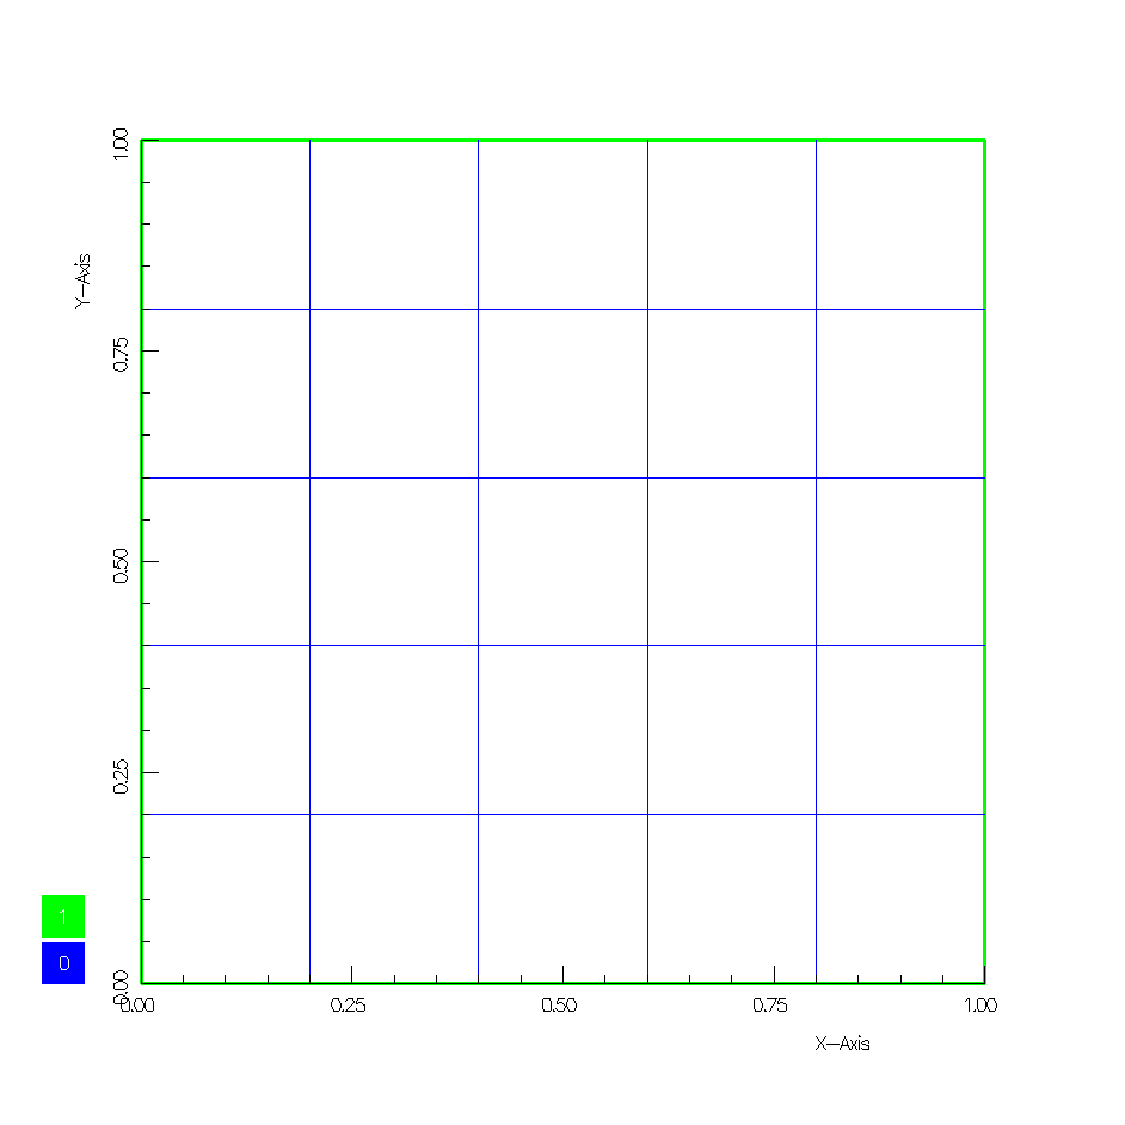
\epsfig{file=\figures/square.ps,height=4.0in} \\
   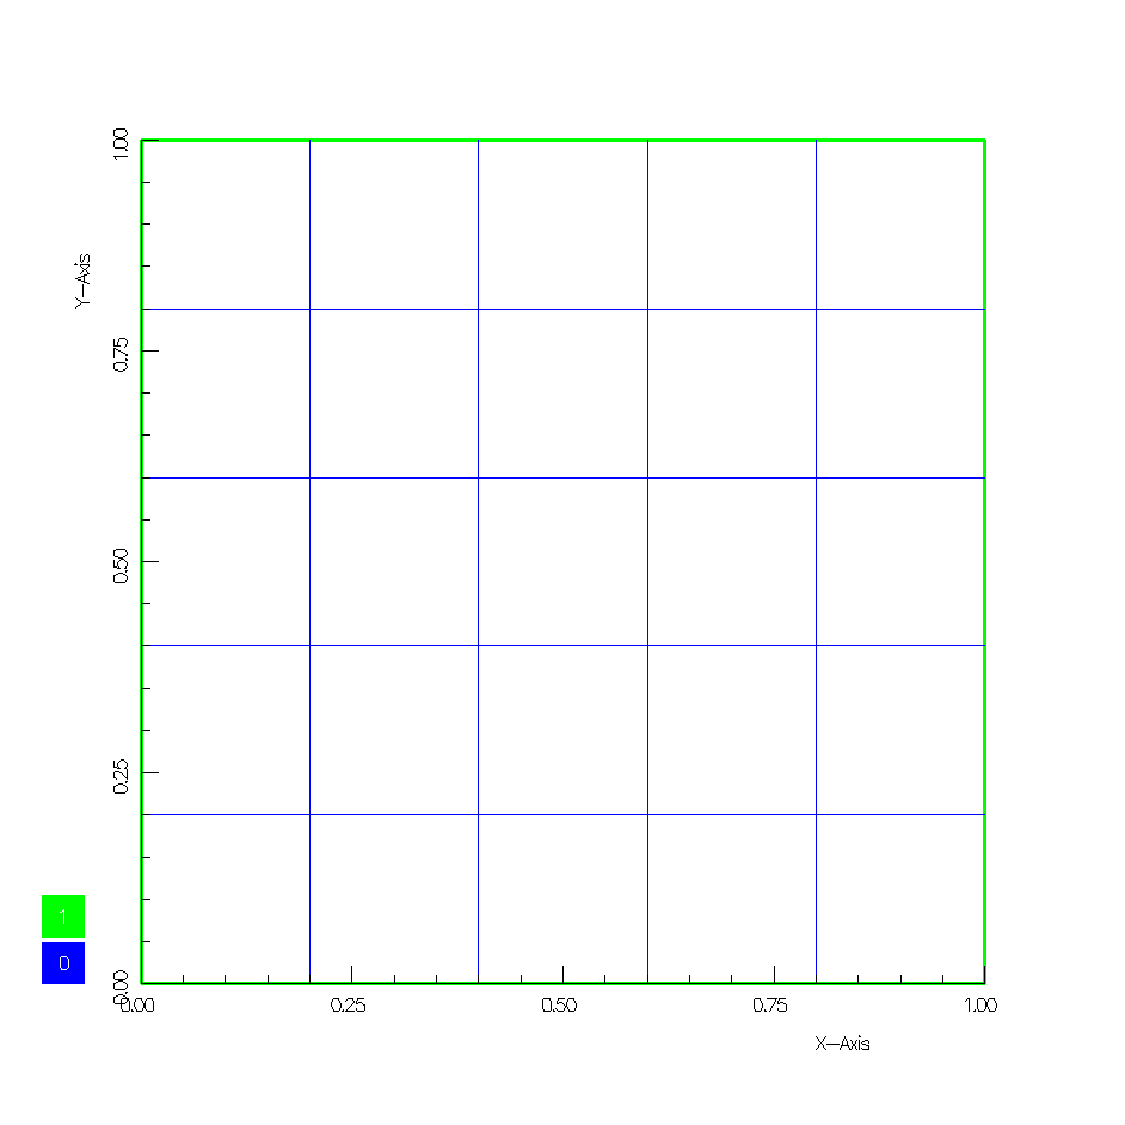
\includegraphics[height=4.0in]{\figures/square} \\
    {An ``overlapping grid'' that is just a square}  \label{fig:square}
  \end{center}
\end{minipage}


\clearpage
\subsection{Stretched Annulus}

FAQ :  What the heck is going on with the stretching function?! (F. Olsson-Hector)

\vspace{\baselineskip}
\noindent Answer: Here is a command file to create an annulus with stretching.
(file {\tt Overture/sampleGrids/stretchedAnnulus.cmd})
Grid lines can be stretched in the coordinate directions (i.e. in the unit-square coordinates).
When grid lines are stretched, as in the example below, the graphics screen will show one of the
following
\begin{itemize}
  \item The mapping to be stretched (annulus)
  \item The unit square to be stretched.
  \item The one dimensional stretching function.
\end{itemize}
% 
% The stretching is in a couple of stages. Upon choosing the {\tt transform/stretch coordinates}
% Now choosing the {\tt stretch} option.
% option one is shown the unit square (this is the StrechedSquare Mapping).
% The grid lines can be stretched in one or more directions
% on the unit square. Choosing the {\tt stretch}
% 
The stretching functions are described in the documentation on Mapping's \cite{MAPPINGS}.

\vspace{\baselineskip}
\begin{minipage}{.4\linewidth}
{\footnotesize
\listinginput[1]{1}{\ogen /stretchedAnnulus.cmd}
}
\end{minipage}\hfill
\begin{minipage}{.6\linewidth}
  \begin{center}
   % 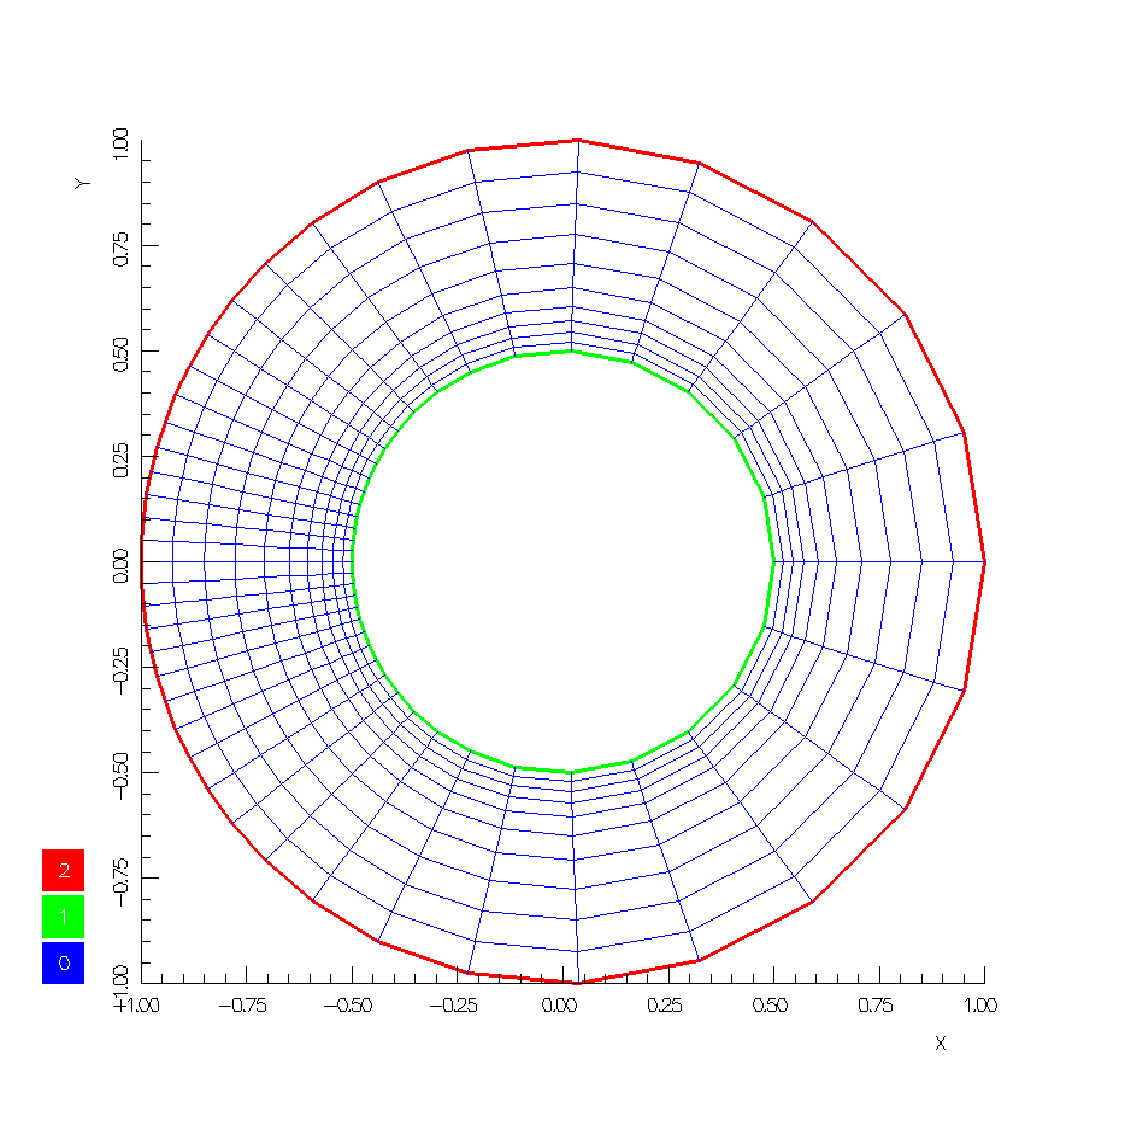
\epsfig{file=\figures/stretchedAnnulus.ps,height=4.0in} \\
   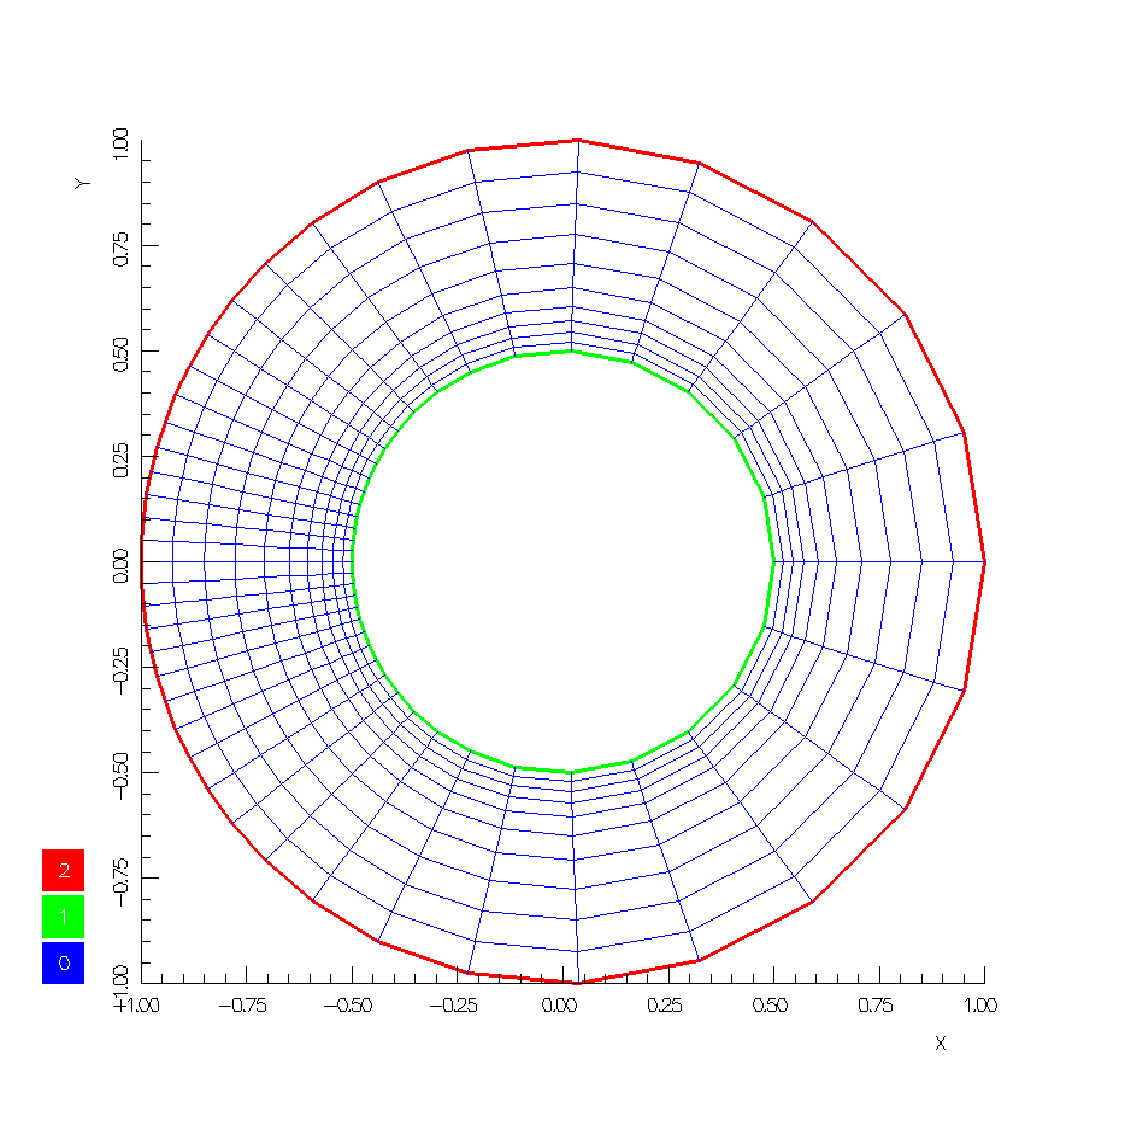
\includegraphics[height=4.0in]{\figures/stretchedAnnulus}
    {An annulus with stretching}  \label{fig:stretchedSquare}
  \end{center}
\end{minipage}

\vspace{\baselineskip}
\noindent For the pundits: The stretched annulus is a {\tt StretchTransform} Mapping which is
a composition of the {\tt StretchedSquare} Mapping and the {\tt Annulus} Mapping.
The {\tt StretchedSquare} uses the {\tt Stretch} Mapping where the actual one dimensional
stretching functions are defined.


\clearpage
\subsection{Cylinder in a channel}\label{sec:cylinderInAChannel}

Here is a command file to create a cylinder in a channel.
(file {\tt Overture/sampleGrids/cic.cmd})
In this case we make two mappings, one a background grid and one an
annulus. The boundary conditions on the annulus are set so that
the outer boundary is an interpolation boundary (=0) while the
boundary conditions on the branch cut are $-1$ to indicate a periodic
boundary. We show two overlapping grids, one made with implicit interpolation (default)
and one made with explicit interpolation. The latter has a bigger region of overlap.
%The resulting grid is shown in figure~\ref{fig:cic}.

\begin{minipage}{.4\linewidth}
{\footnotesize
\listinginput[1]{1}{\ogen /cic.cmd}
}
\end{minipage}\hfill
\begin{minipage}{.6\linewidth}
  \begin{center}
   % 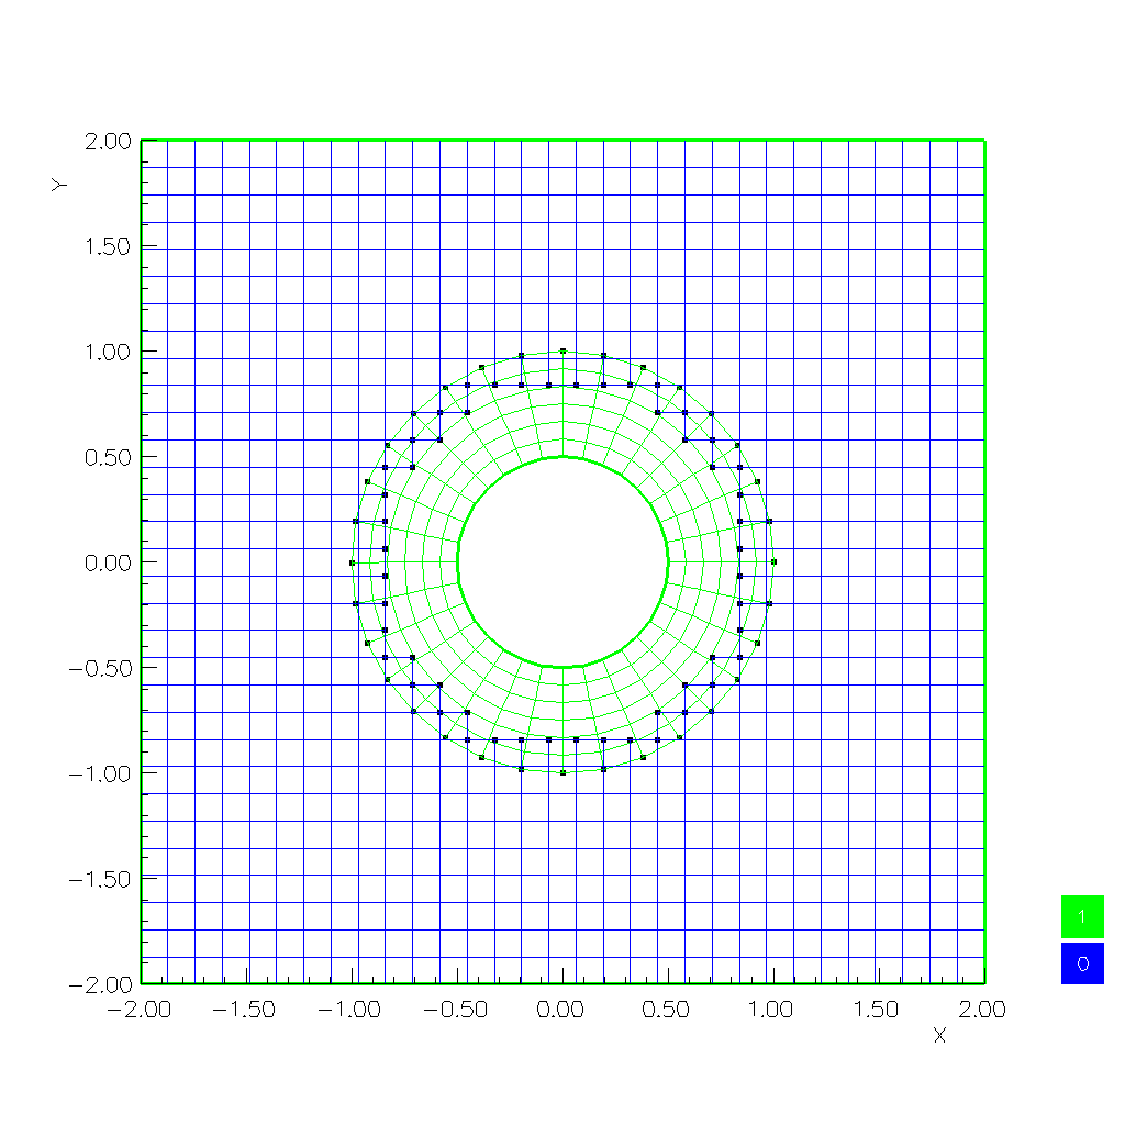
\epsfig{file=\figures/cicImplicit.ps,height=3.5in}  \\
   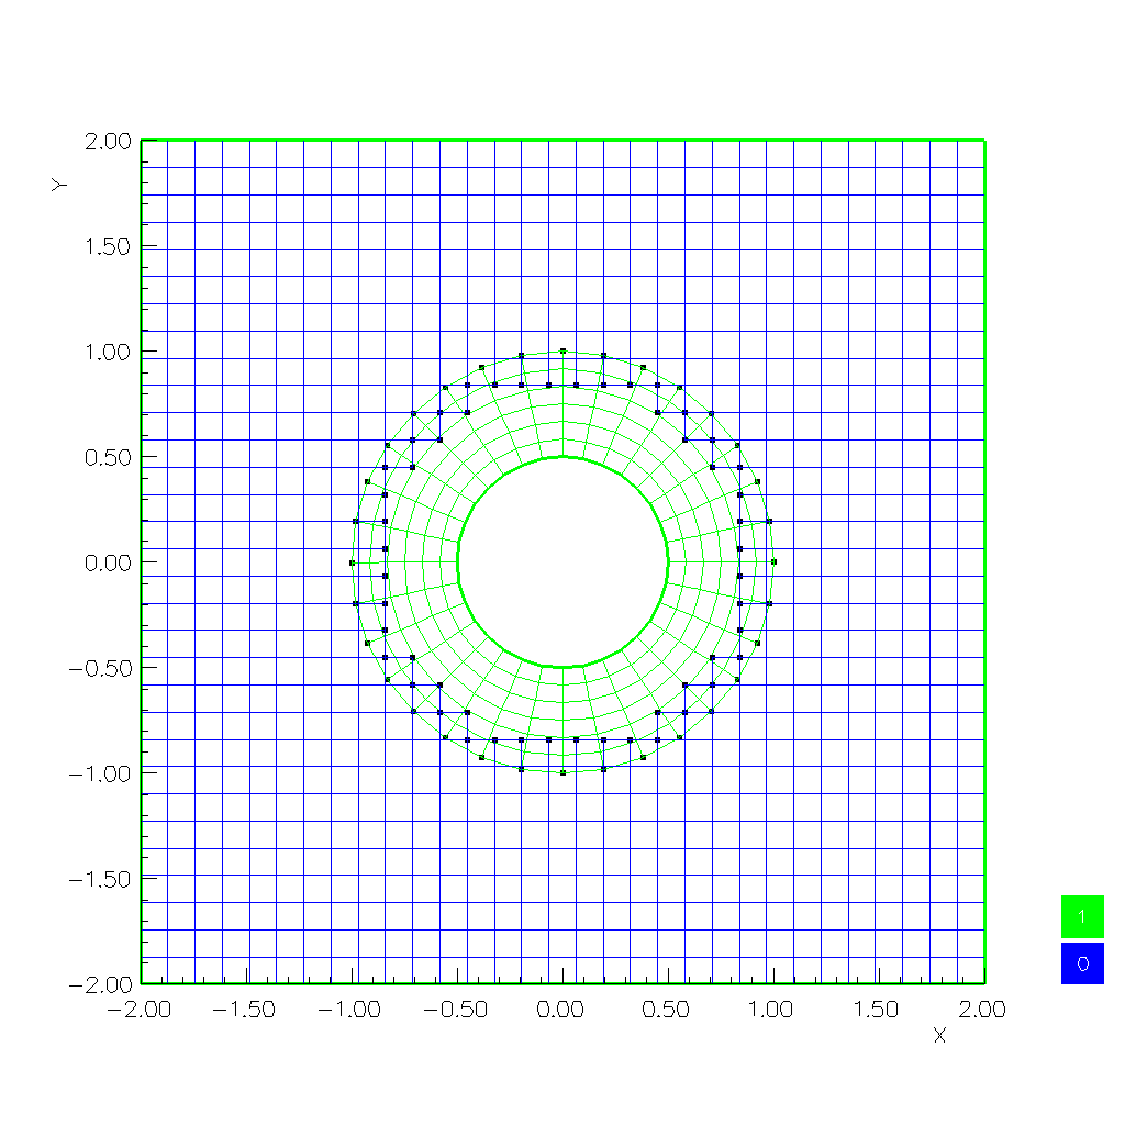
\includegraphics[height=3.5in]{\figures/cicImplicit}\\
  {An overlapping grid for a cylinder in a channel with implicit interpolation}  
   % 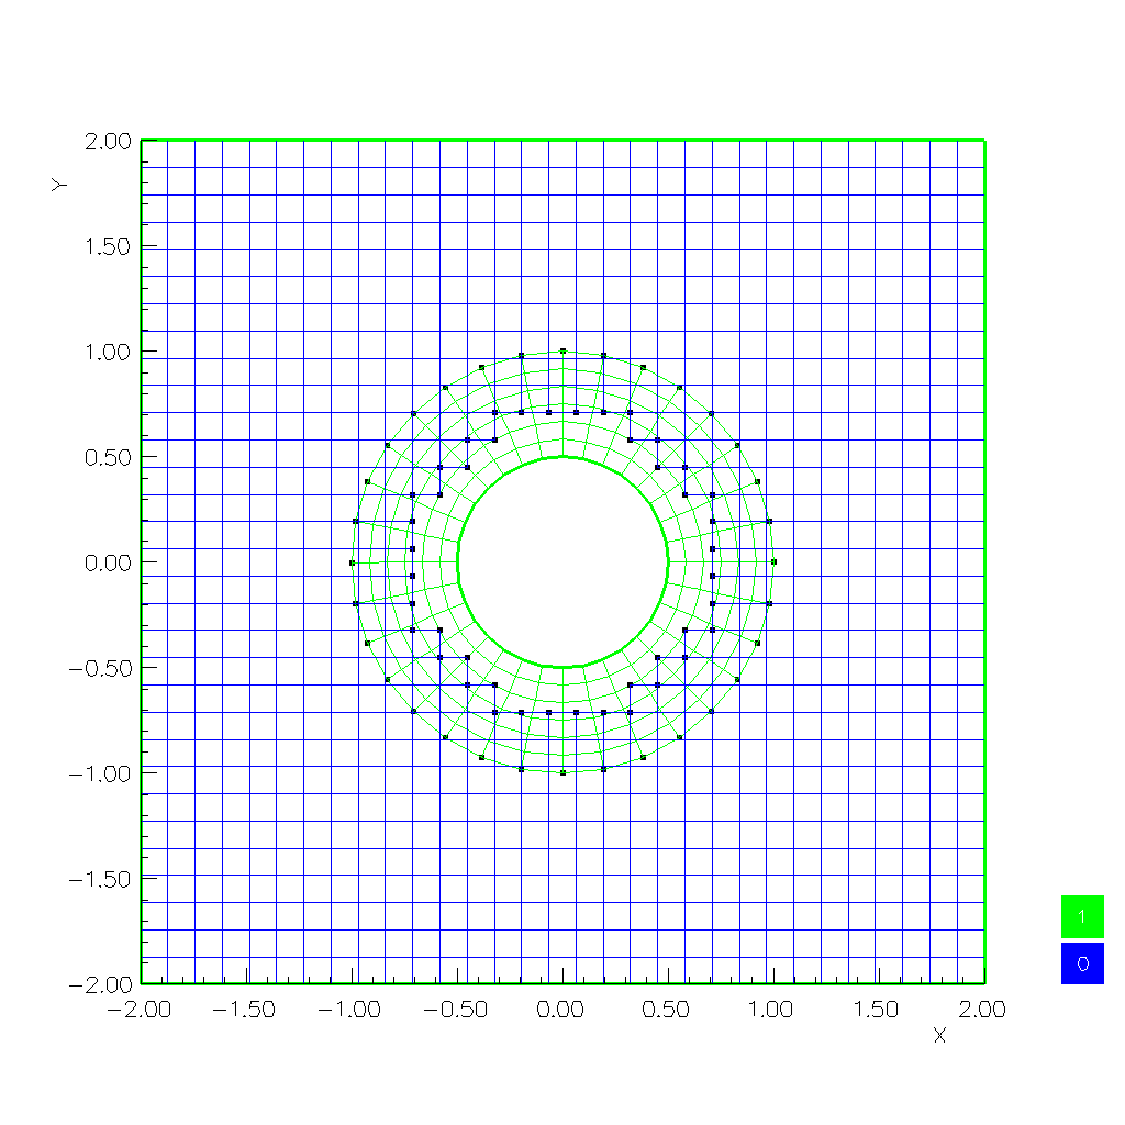
\epsfig{file=\figures/cicExplicit.ps,height=3.5in}  \\
   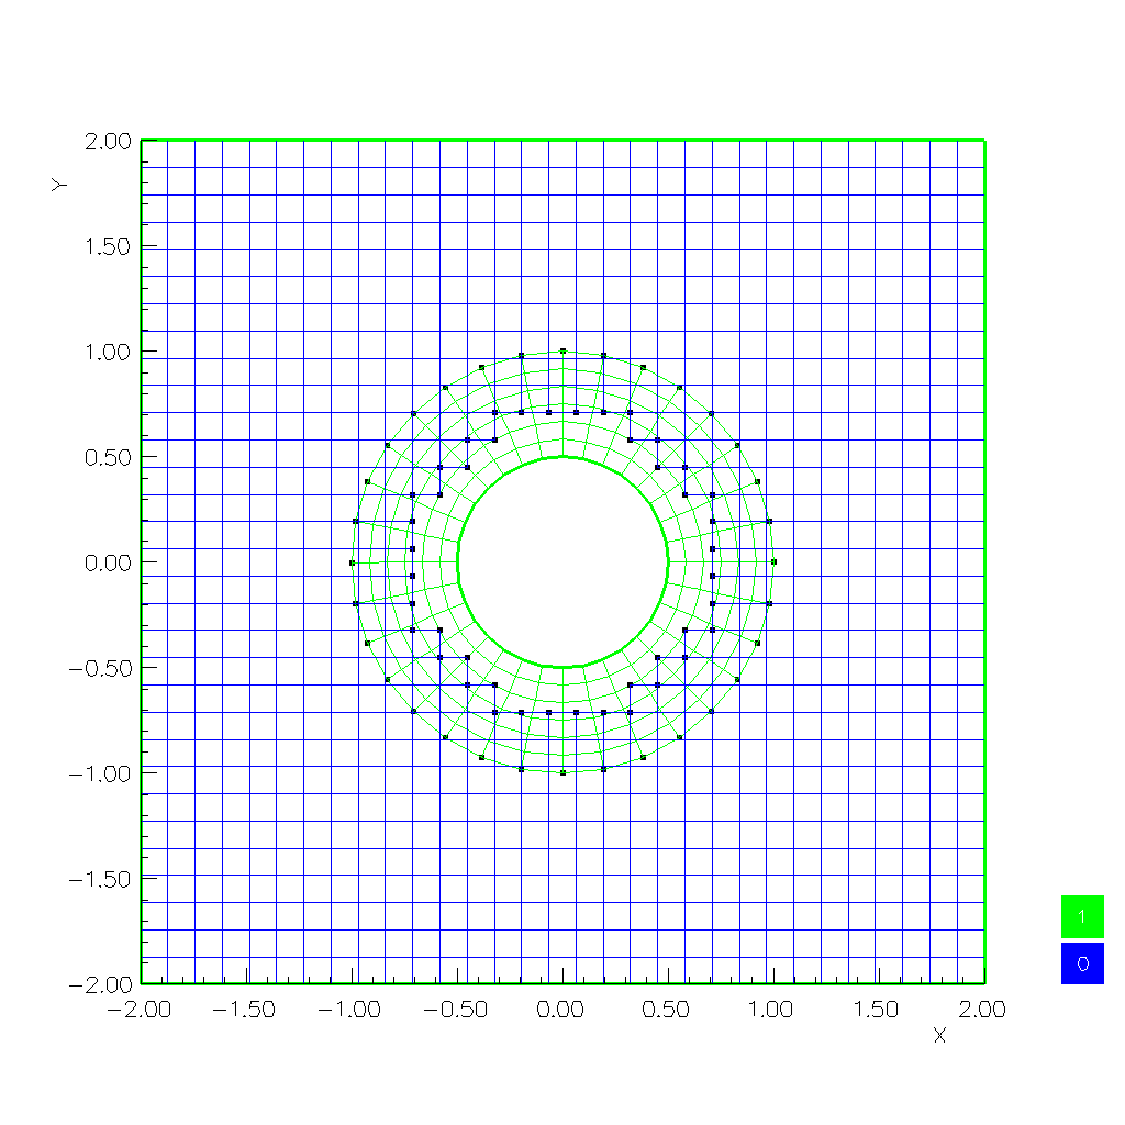
\includegraphics[height=3.5in]{\figures/cicExplicit}\\
  {An overlapping grid for a cylinder in a channel with explicit interpolation}  \label{fig:cic}
  \end{center}
\end{minipage}

\clearpage
\subsection{Cylinder in a channel, cell-centered version }\label{sec:cylinderInAChannelCC}

Here we repeat the last example but create a cell-centered grid. 
In a cell-centered grid the cell-centres of one grid are interpolated
from the cell-centres of another grid. For this reason the cell-centred grid requires
slighly more overlap between the component grids.

{\bf Note:} Most of the solvers in Overture use vertex-centered grids instead of cell centered grids.
This is true even with the finite volume solvers in which case the grid vertex represents the center
of the computational cell. 

\begin{minipage}{.4\linewidth}
{\footnotesize
\listinginput[1]{1}{\ogen /cicCC.cmd}
}
\end{minipage}\hfill
\begin{minipage}{.6\linewidth}
  \begin{center}
   % 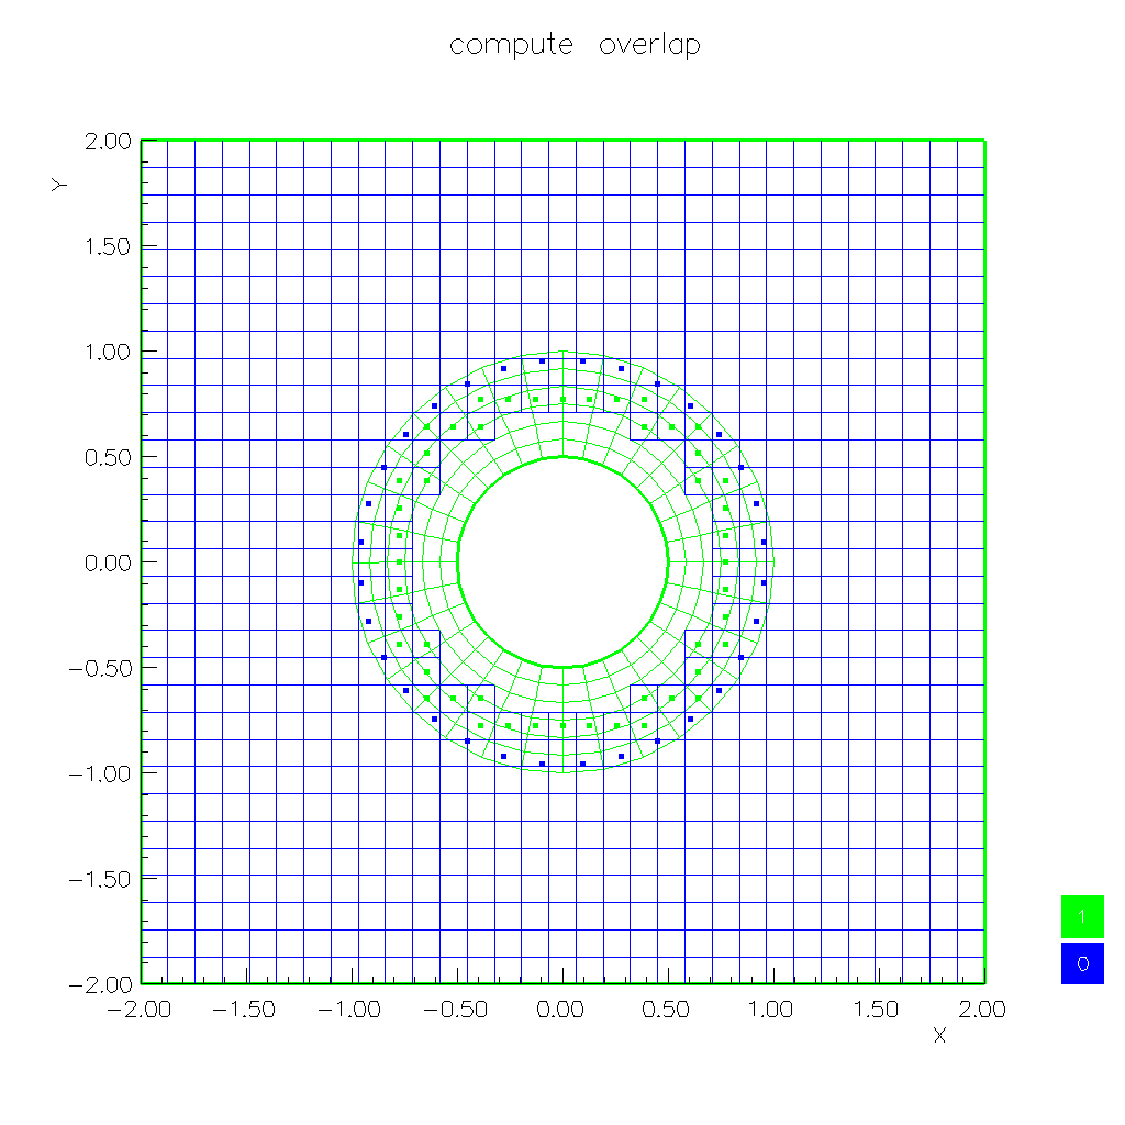
\epsfig{file=\figures/cicCC.ps,height=4.5in}  \\
   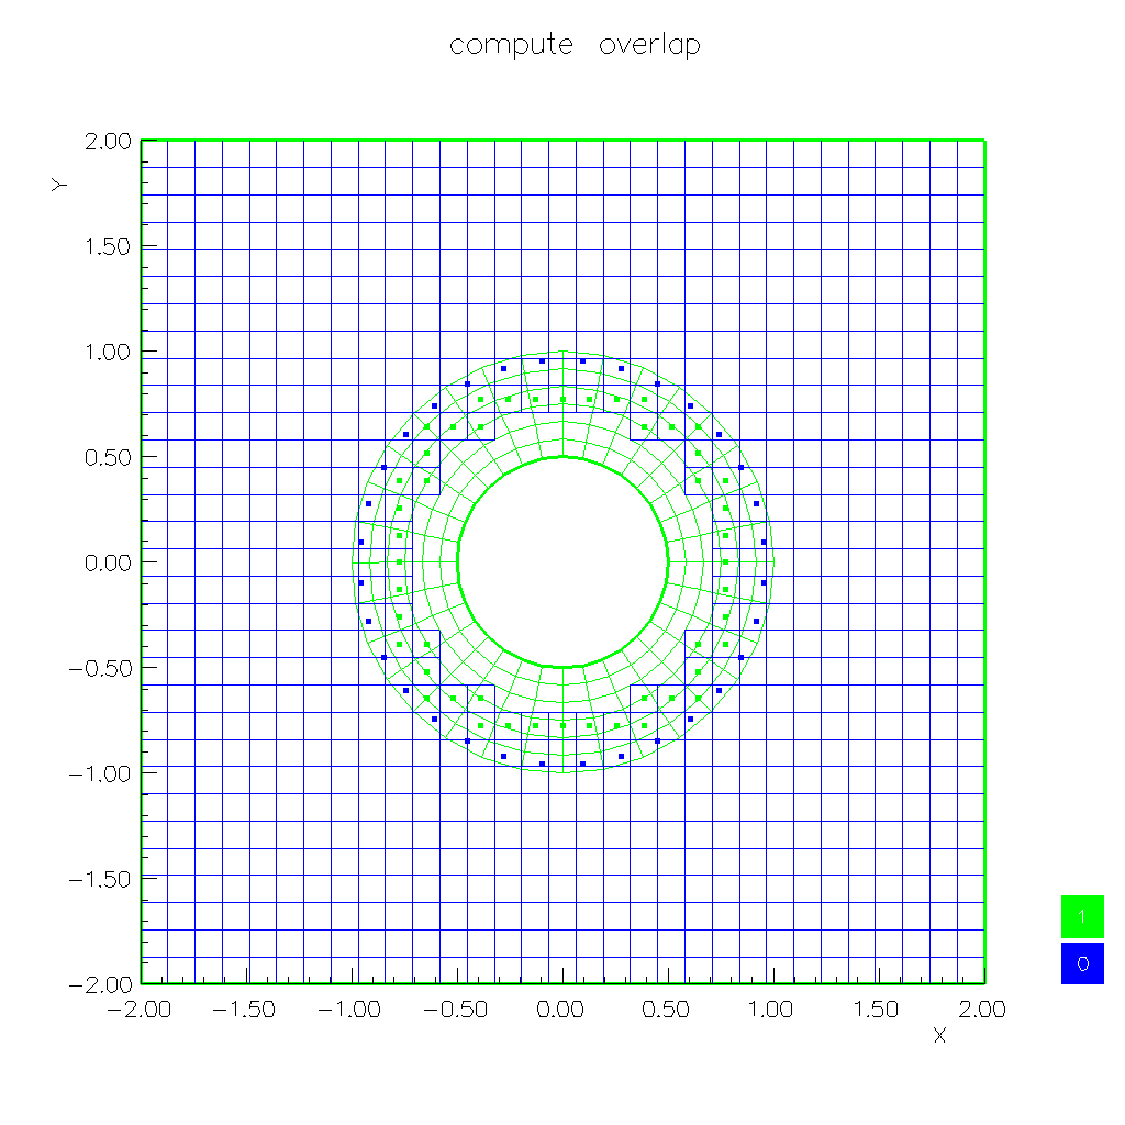
\includegraphics[height=4.5in]{\figures/cicCC}\\
  {An overlapping grid for a cylinder in a channel, cell-centered case.}  \label{fig:cicCC}
  \end{center}
\end{minipage}


% ----------------------------------------------------------------------------------------------
\clearpage
\subsection{Cylinder in a channel, fourth-order version }\label{sec:cylinderInAChannelFour}

Here we repeat the last example but create a grid appropriate for a fourth-order
discretization. We need to increase the discretization width to 5 and the interpolation
width to 5. This can either be done explicitly or the option ``{\tt order of accuracy}''
can be used.
Notice that two lines of interpolation points are generated as required
by the wider stencil.
%
\begin{multicols}{2}
{\footnotesize
\listinginput[1]{1}{\ogen/cic.4.cmd}
}
\end{multicols}
% 
  \begin{center}
   % \epsfig{file=\figures/cic.4.ps,height=4.5in}  \\
   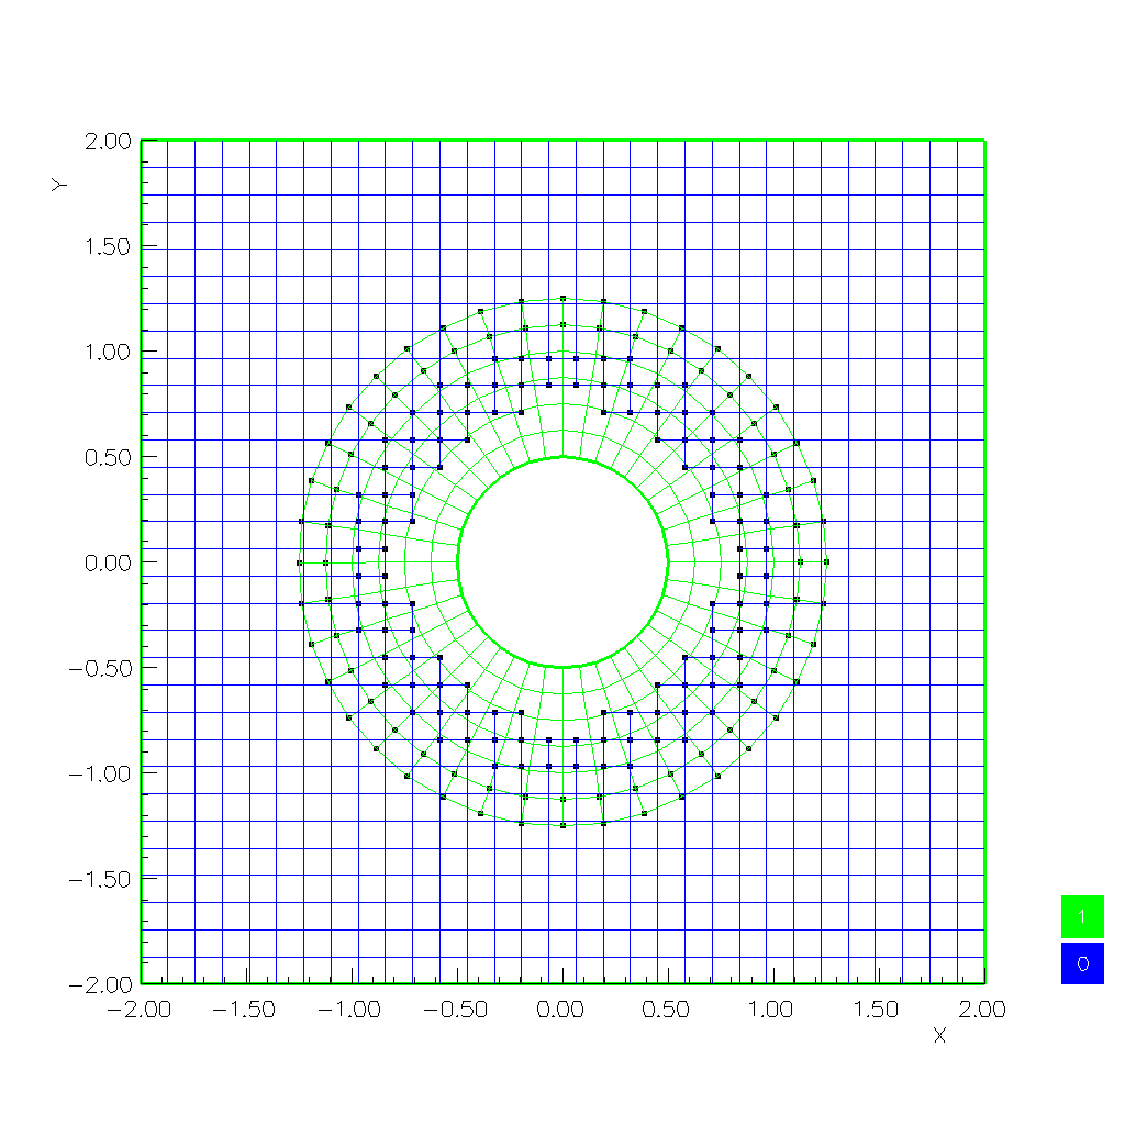
\includegraphics[height=3.5in]{\figures/cic_4}\\
  {An overlapping grid for a cylinder in a channel, fourth-order case.}  \label{fig:cicFour}
  \end{center}


% % ----------------------------------------------------------------------------------------------
% \clearpage
% \subsection{Cylinder in a channel, multigrid version }\label{sec:cylinderInAChannelMG}
% 
% Here we make a grid that can be used with a multigrid solver. The only difference in the
% command file is that we must specify how many multigrid levels we require. {\bf NOTE} that
% since each multigrid level must be a valid overlapping grid you cannot expect to have more than
% a few levels. See the examples in the primer for how to access the different multigrid levels
% in a {\tt CompositeGrid}.
% %  and see the documentation for the multigrid solver 
% 
%    
% 
% \noindent
% \begin{minipage}{.4\linewidth}
% {\footnotesize
% \listinginput[1]{1}{\ogen /cicmg.cmd}
% }
% \end{minipage}\hfill
% \begin{minipage}{.6\linewidth}
%   \begin{center}
%    \epsfig{file=\figures/cicmg0.ps,height=4.in}  \\
%   {An overlapping grid for a cylinder in a channel, multigrid level 0.}  
%    \epsfig{file=\figures/cicmg1.ps,height=4.in}  \\
%   {An overlapping grid for a cylinder in a channel, multigrid level 1.}
%   \end{center}
% \end{minipage}


% ----------------------------------------------------------------------------------------------
\clearpage
\subsection{Inlet-outlet}\label{sec:inletOutlet}

In this example we demonstrate
\begin{description}
  \item[share flags:] to specify that two component grids have sides that belong
        to the same physical boundary curve. This prevents one physical boundary
        from accidently cutting a hole on a grid that shares the same boundary.
  \item[no hole cutting:] turn off hole cutting to prevent physical boundaries from
     cutting holes in some other grids.
  \item[view mappings:] the mappings can be plotted with boundaries coloured by 
     the boundary condition values or coloured by the share flag values. This 
     allows one to check that the values have been set properly.
\end{description}
This grid is remarkably similar to a grid created by Anders Petersson.


Here is a command file to create the grid for the inlet-outlet example.
(file {\tt \sampleGrids/inletOutlet.cmd}). 
\begin{multicols}{2}
{\footnotesize
\listinginput[1]{1}{\ogen /inletOutlet.cmd}
}
\end{multicols}


{
\newcommand{\figWidthd}{12cm}
\newcommand{\trimfig}[2]{\trimPlot{#1}{#2}{.0}{.0}{.125}{.3}}
\begin{figure}[hbt]
\begin{center}
\begin{tikzpicture}[scale=1]
  \useasboundingbox (0,.75) rectangle (12.,7.5);  % set the bounding box (so we have less surrounding white space)
%
  \draw ( 0.0,0.) node[anchor=south west,xshift=-4pt,yshift=+0pt] {\trimfig{\figures/inletOutletBC}{\figWidthd}};
% grid:
%  \draw[step=1cm,gray] (0,0) grid (12,7.5);
\end{tikzpicture}
\end{center}
  \caption{Inlet-outlet mappings plotted from the ``view mappings'' menu, 
          showing boundary condition values. Physical boundaries have a positive value (1=green),
         interpolation boundaries have a value of zero (0=blue) and periodic boundaries have a 
      negative value (shown in black). }  \label{fig:inletOutletBC}
\end{figure}
% -----------------------------------------------
\begin{figure}[hbt]
\begin{center}
\begin{tikzpicture}[scale=1]
  \useasboundingbox (0,.75) rectangle (12.,7.5);  % set the bounding box (so we have less surrounding white space)
%
  \draw ( 0.0,0.) node[anchor=south west,xshift=-4pt,yshift=+0pt] {\trimfig{\figures/inletOutletShare}{\figWidthd}};
% grid:
% \draw[step=1cm,gray] (0,0) grid (12,7.5);
\end{tikzpicture}
\end{center}
  \caption{Inlet-outlet mappings plotted from the ``view mappings'' menu, 
          showing shared side values. Grids that share the same physical boundary should
     have the same value of the share flag. For example, the two inlet grids on the right
     share boundaries with the back-ground grid (value 2=red). The inlet grids also share
      boundaries with each other (value 5) }  \label{fig:inletOutletShare}
\end{figure}
% -----------------------------------------------
\begin{figure}[hbt]
\begin{center}
\begin{tikzpicture}[scale=1]
  \useasboundingbox (0,.75) rectangle (12.,7.5);  % set the bounding box (so we have less surrounding white space)
%
  \draw ( 0.0,0.) node[anchor=south west,xshift=-4pt,yshift=+0pt] {\trimfig{\figures/inletOutlet}{\figWidthd}};
% grid:
% \draw[step=1cm,gray] (0,0) grid (12,7.5);
\end{tikzpicture}
\end{center}
  \caption{Inlet-outlet overlapping grid. To create this grid we had to prevent the 
      background grid from cutting holes in the two inlet grids (on the right) and the
      outlet grid on the left. The outlet grid was also prevented from cutting holes in
      the background grid.}  \label{fig:inletOutlet}
\end{figure}
}

% {
% \newcommand{\figWidtha}{7cm}
% \begin{figure}[htb]
%   \begin{center}
%    % 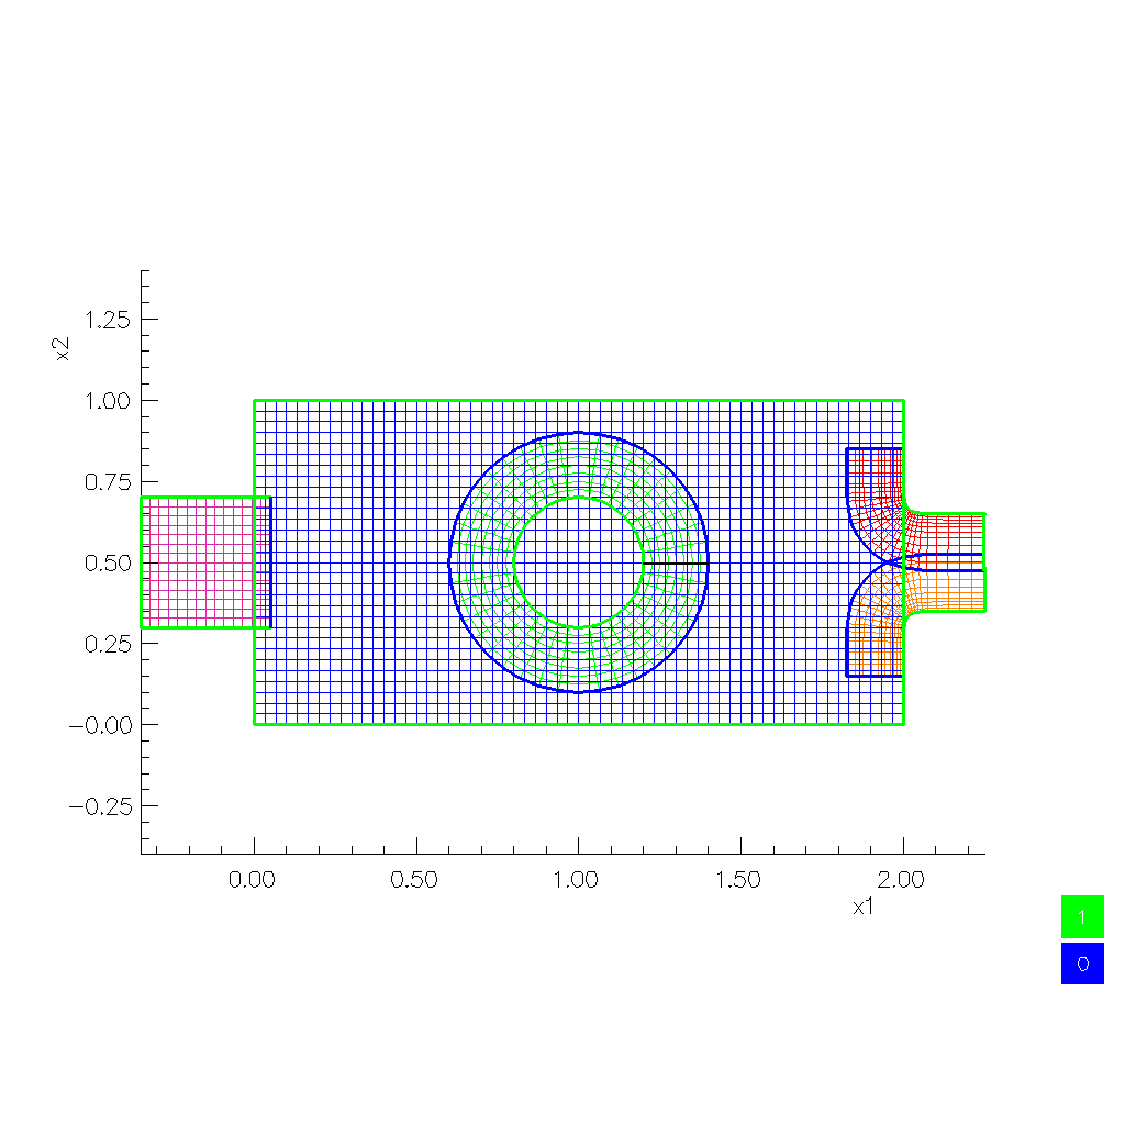
\epsfig{file=\figures/inletOutletBC.ps,clip=,width=.75\linewidth} 
%    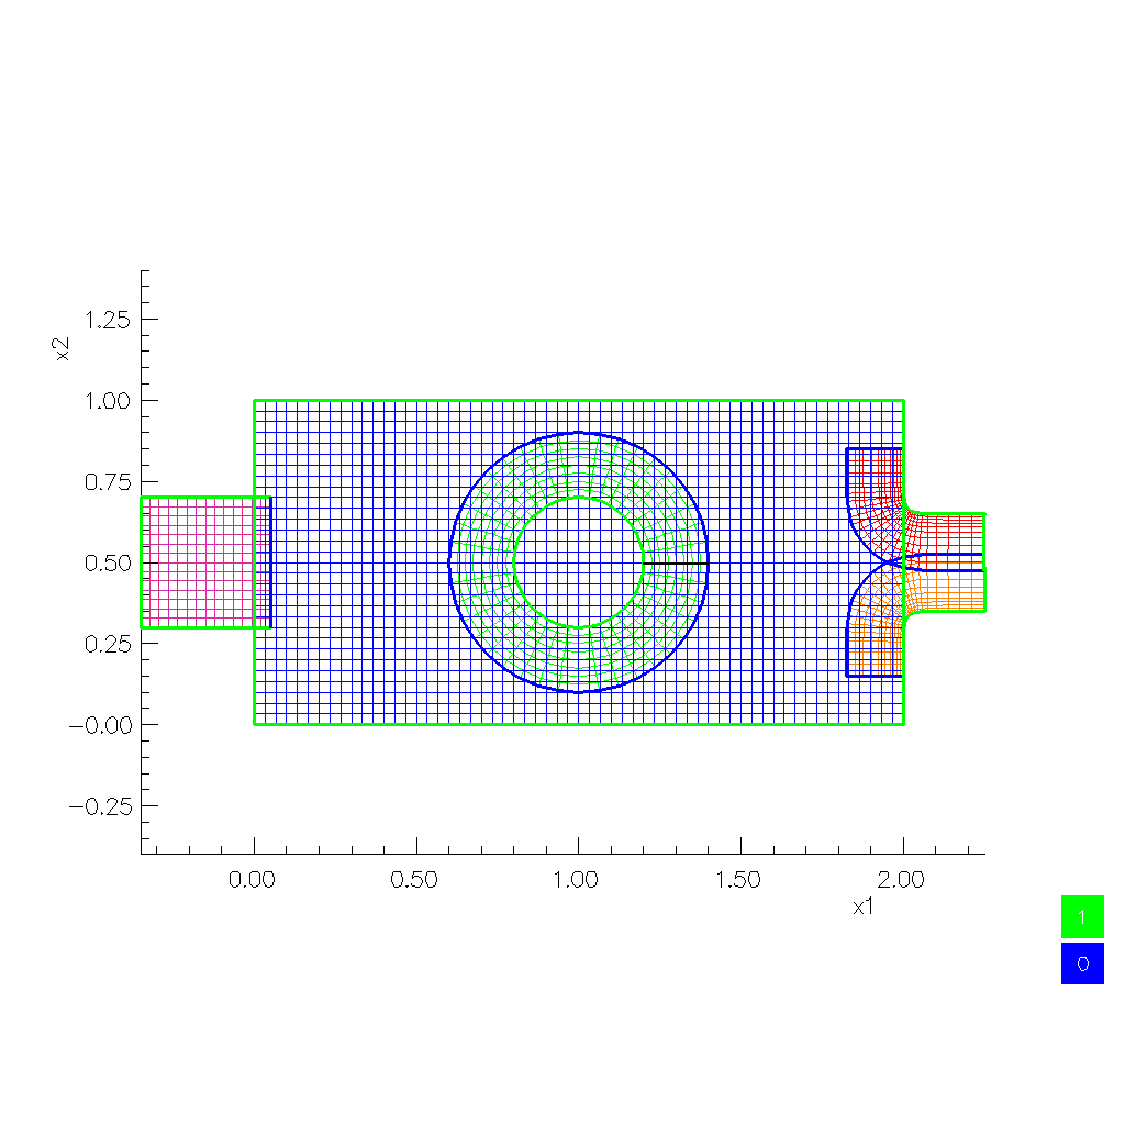
\includegraphics[height=\figWidtha]{\figures/inletOutletBC}\\
%   \caption{Inlet-outlet mappings plotted from the ``view mappings'' menu, 
%           showing boundary condition values. Physical boundaries have a positive value (1=green),
%          interpolation boundaries have a value of zero (0=blue) and periodic boundaries have a 
%       negative value (shown in black). }  \label{fig:inletOutletBC}
%   \end{center}
% \end{figure}
% \begin{figure}[htb]
%   \begin{center}
%    % 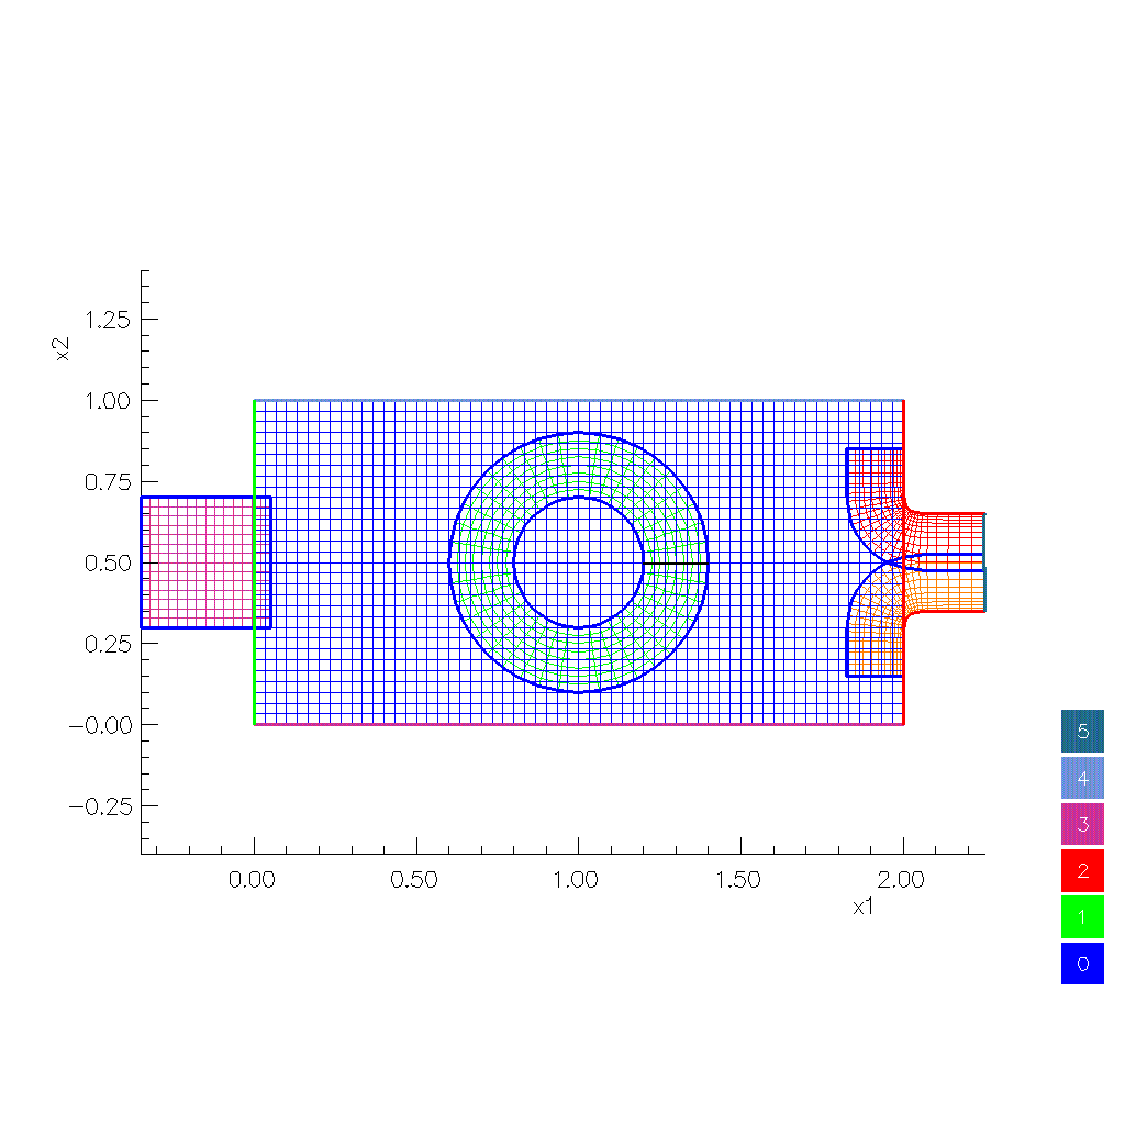
\epsfig{file=\figures/inletOutletShare.ps,clip=,width=.75\linewidth} 
%    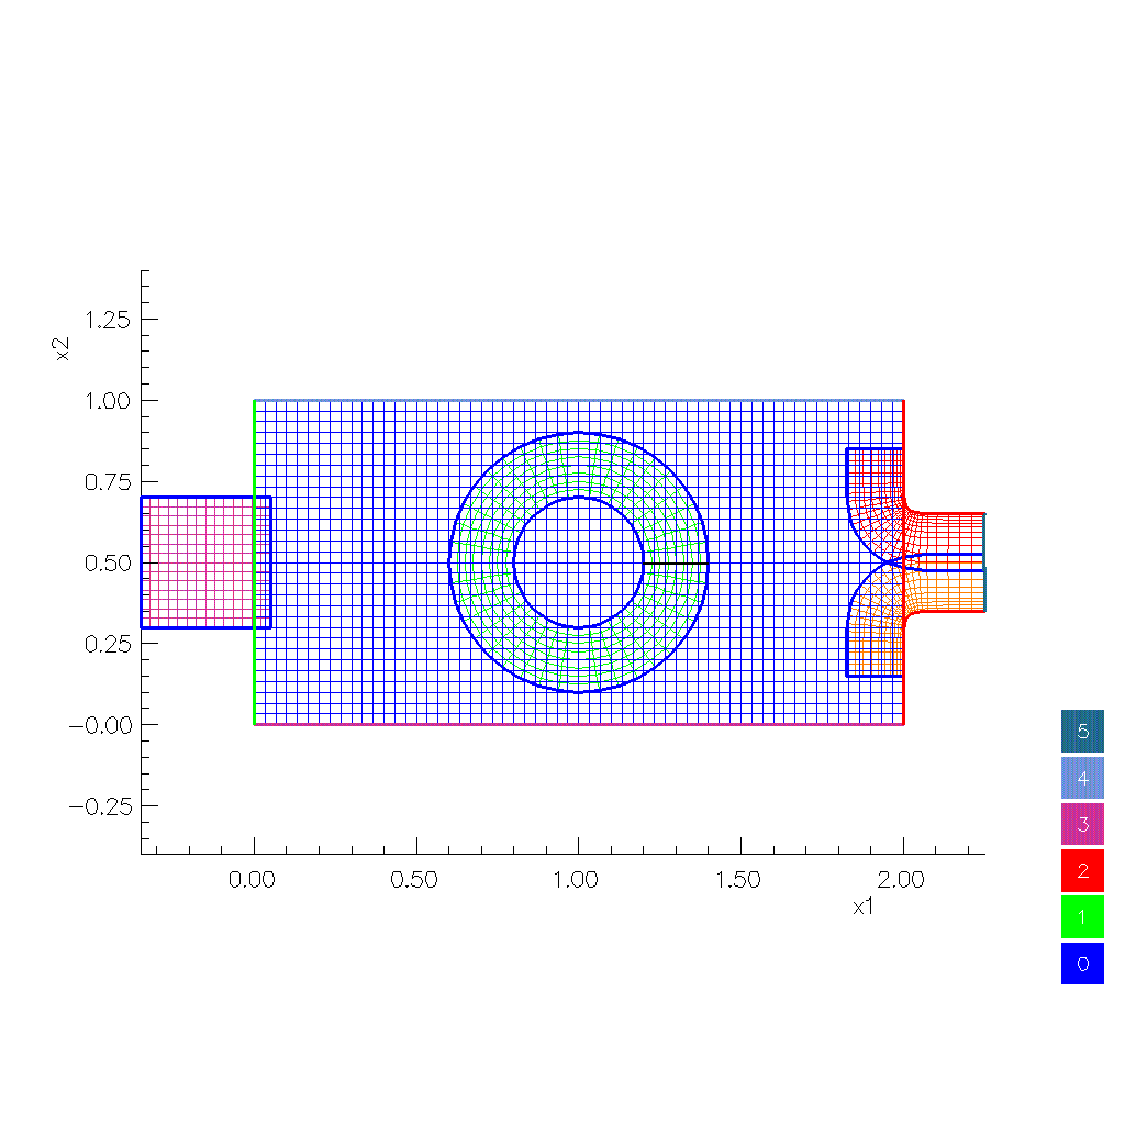
\includegraphics[height=\figWidtha]{\figures/inletOutletShare}\\
%   \caption{Inlet-outlet mappings plotted from the ``view mappings'' menu, 
%           showing shared side values. Grids that share the same physical boundary should
%      have the same value of the share flag. For example, the two inlet grids on the right
%      share boundaries with the back-ground grid (value 2=red). The inlet grids also share
%       boundaries with each other (value 5) }  \label{fig:inletOutletShare}
%   \end{center}
% \end{figure}
% \begin{figure}[htb]
%   \begin{center}
%    % 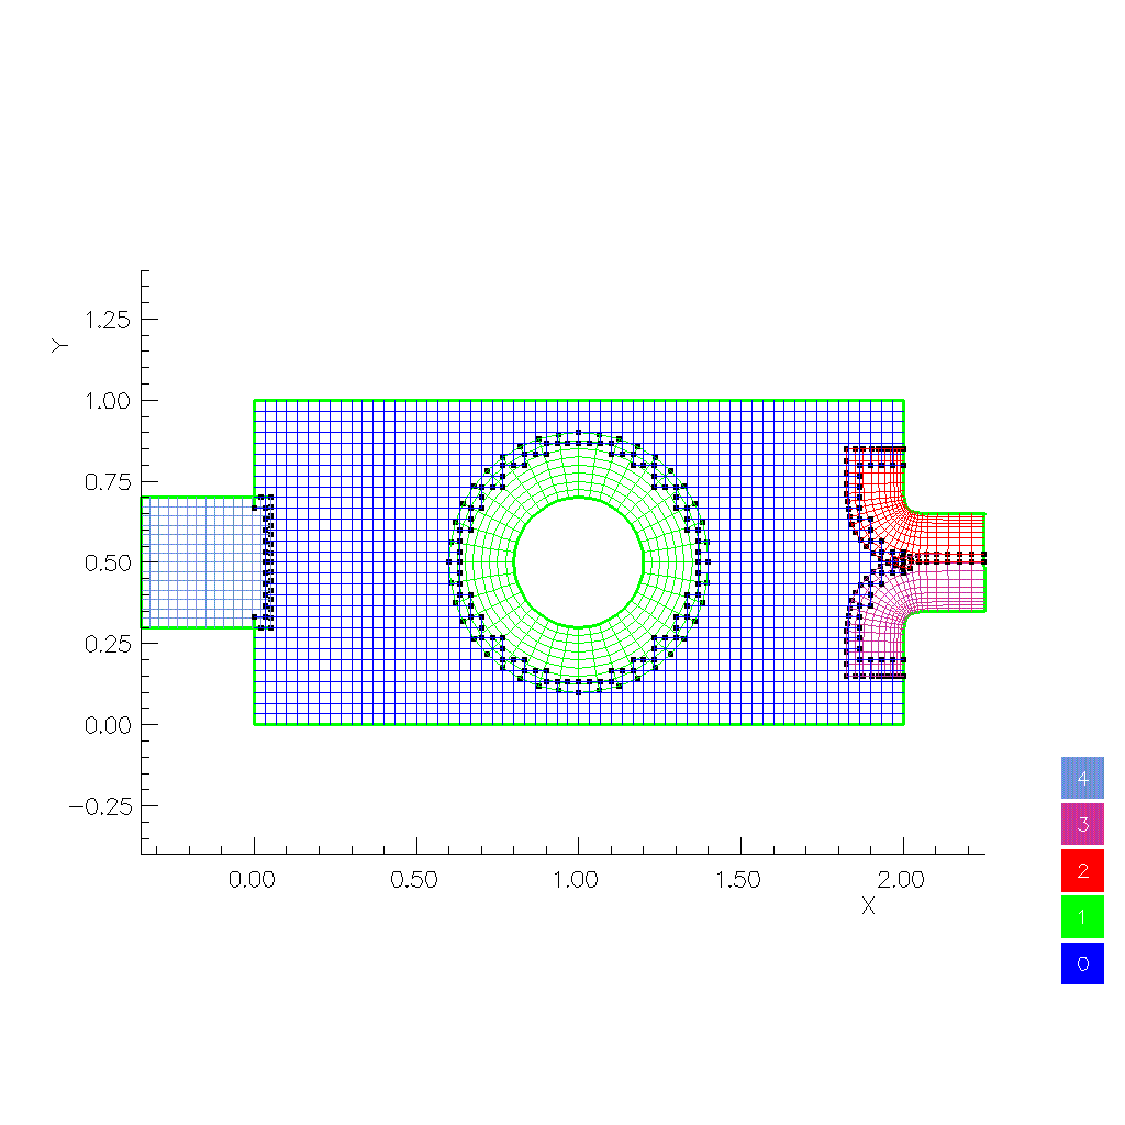
\epsfig{file=\figures/inletOutlet.ps,clip=,width=.75\linewidth} 
%    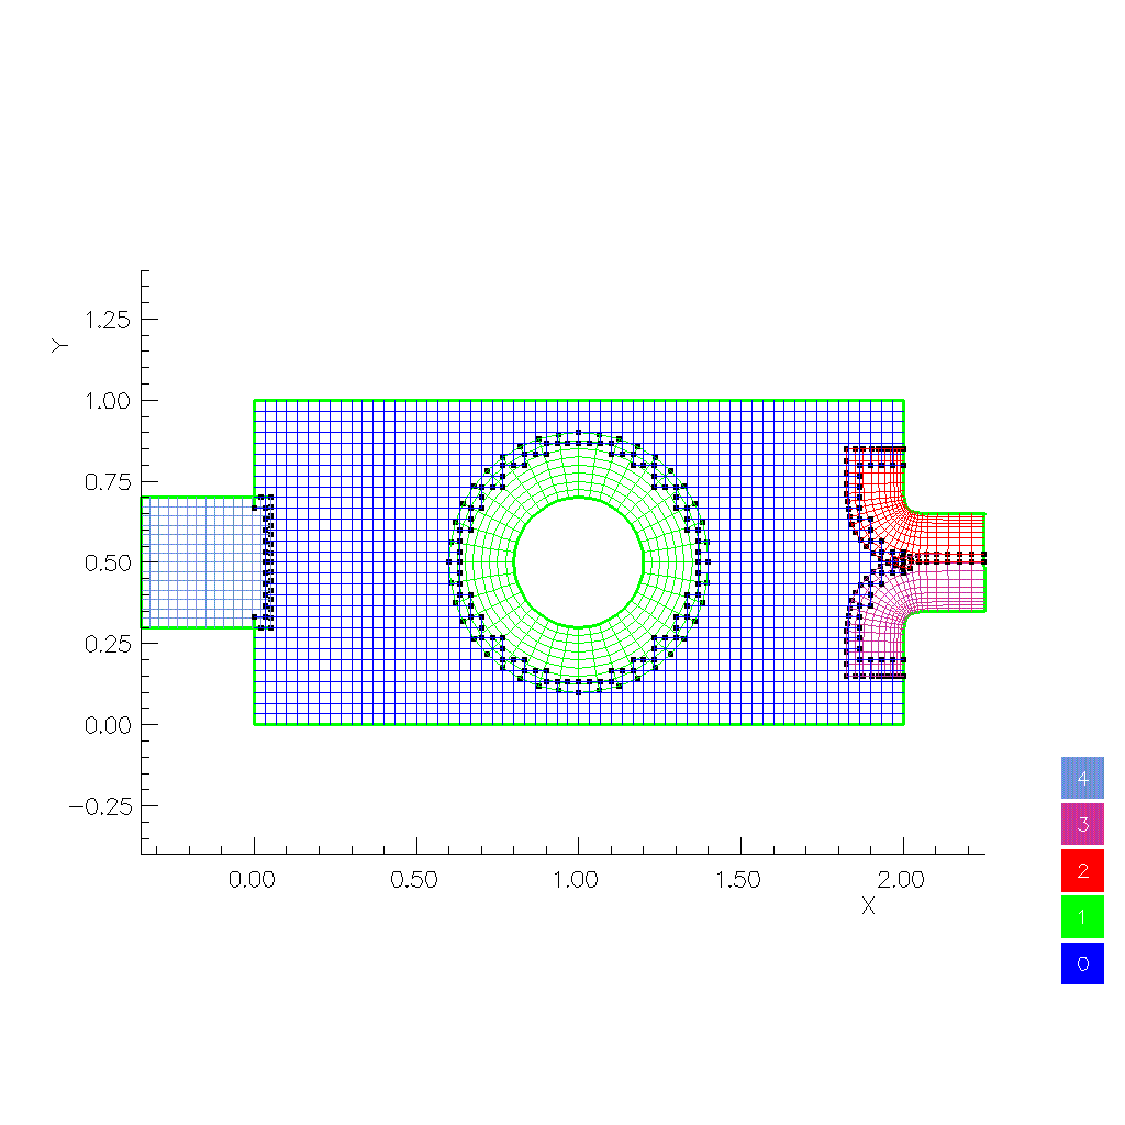
\includegraphics[height=\figWidtha]{\figures/inletOutlet}\\
%   \caption{Inlet-outlet overlapping grid. To create this grid we had to prevent the 
%       background grid from cutting holes in the two inlet grids (on the right) and the
%       outlet grid on the left. The outlet grid was also prevented from cutting holes in
%       the background grid.}  \label{fig:inletOutlet}
%   \end{center}
% \end{figure}
% }
The cell-centred version may be created with {\tt \sampleGrids/inletOutlet.cmd}.

% ------------------------------------------------------------------------------------------------------------
\clearpage
\subsection{Valve}

Here is a command file to create a grid around a two-dimensional valve
(file {\tt \sampleGrids/valve.cmd}). 
\begin{multicols}{2}
{\footnotesize
\listinginput[1]{1}{\ogen /valve.cmd}
}
\end{multicols}

The resulting grid is shown in figure~\ref{fig:valve}.
\begin{figure}[htb]
  \begin{center}
%   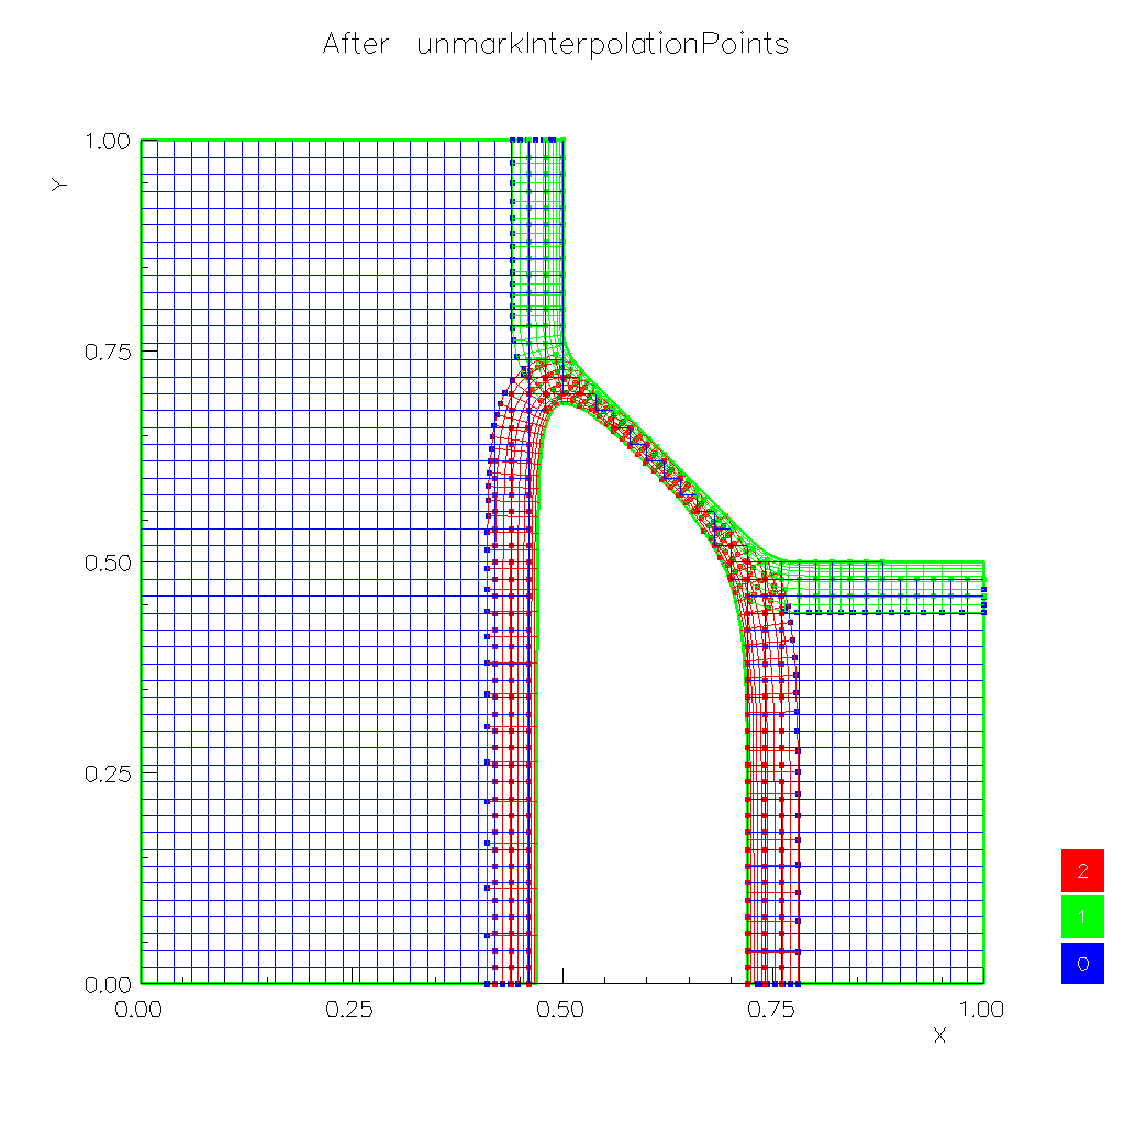
\epsfig{file=\figures/valveDone.ps,height=6.0in}
   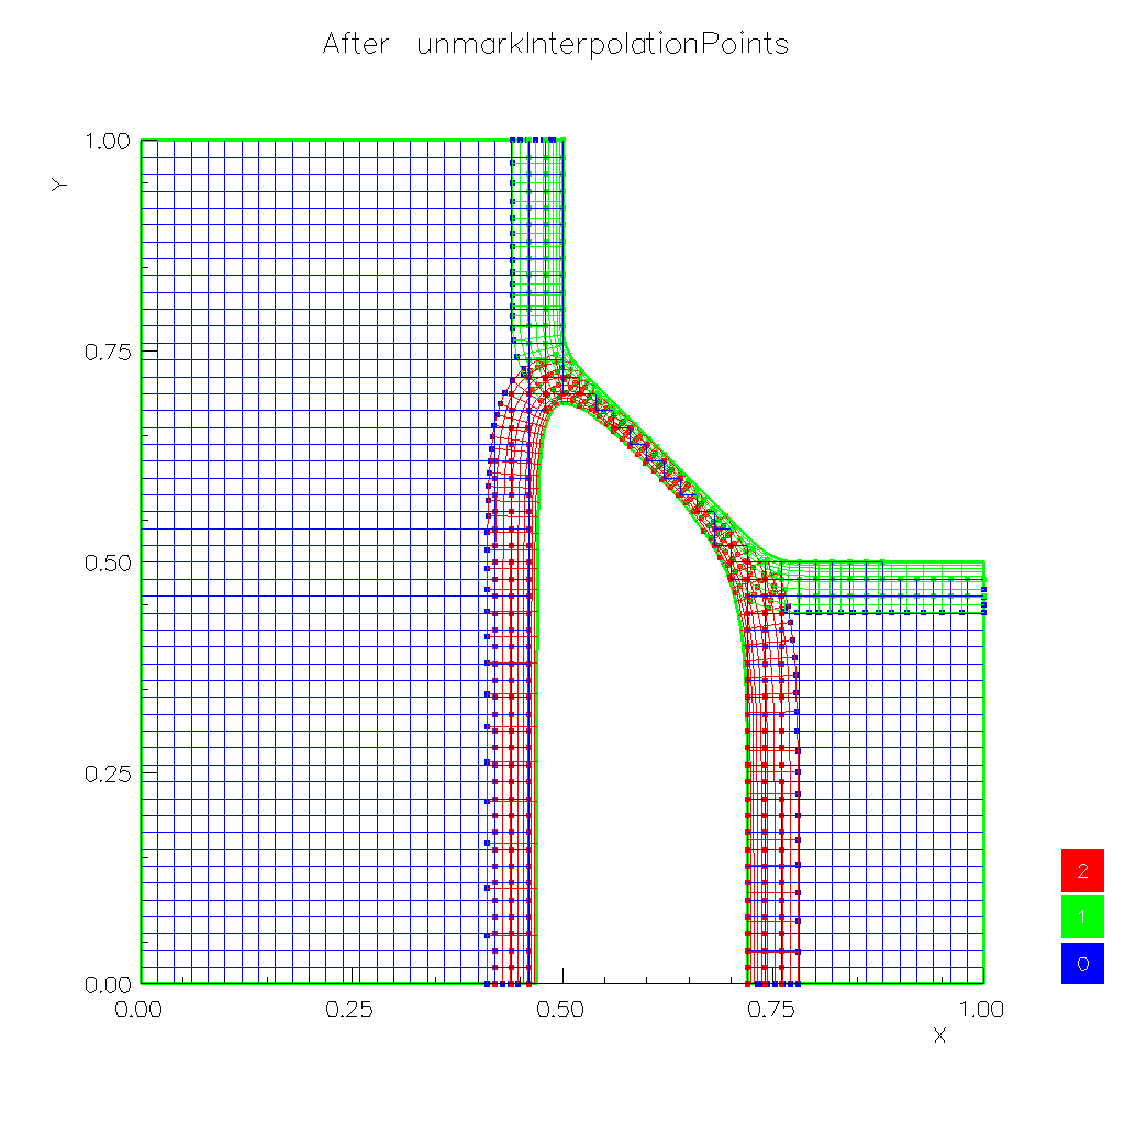
\includegraphics[height=6.0in]{\figures/valveDone}\\
  \caption{An overlapping grid for a valve}  \label{fig:valve}
  \end{center}
\end{figure}
The cell centered version may be created with {\tt \sampleGrids/valveCC.cmd}.

\clearpage
\subsection{NACA airfoil}\index{airfoil}\index{mapping!AirFoilMapping}

Here is a command file to create a grid around a two-dimensional NACA0012 airfoil
(file {\tt Overture\-/sampleGrids\-/naca0012.cmd}). The airfoil curve is created first with
the {\tt AirfoilMapping} (see the Mapping documentation for an explanation of
NACA 4 digit airfoils). This curve is blended with an ellipse (using 
transfinite interpolation) to make an initial grid. The transfinite interpolation 
mapping\index{mapping!transfinite interpolation}
then then smoothed
using elliptic grid generation to form the airfoil grid.
\begin{multicols}{2}
{\footnotesize
\listinginput[1]{1}{\ogen /naca0012.cmd}
}
\end{multicols}

The resulting grid is shown in figure~\ref{fig:naca0012}.
\begin{figure}[htb]
  \begin{center}
   % 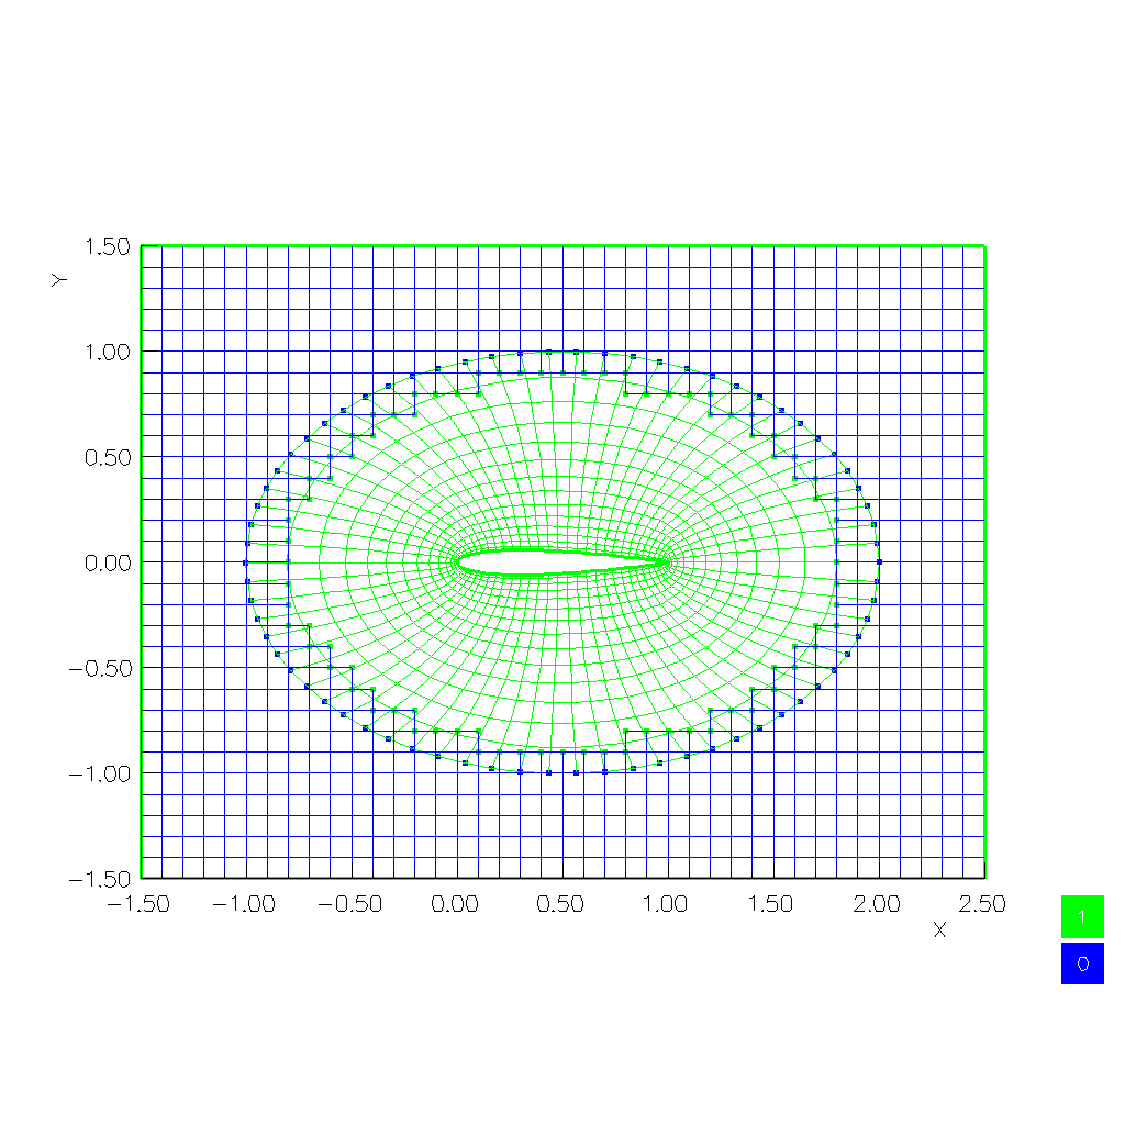
\epsfig{file=\figures/naca0012.ps,height=6.0in}
   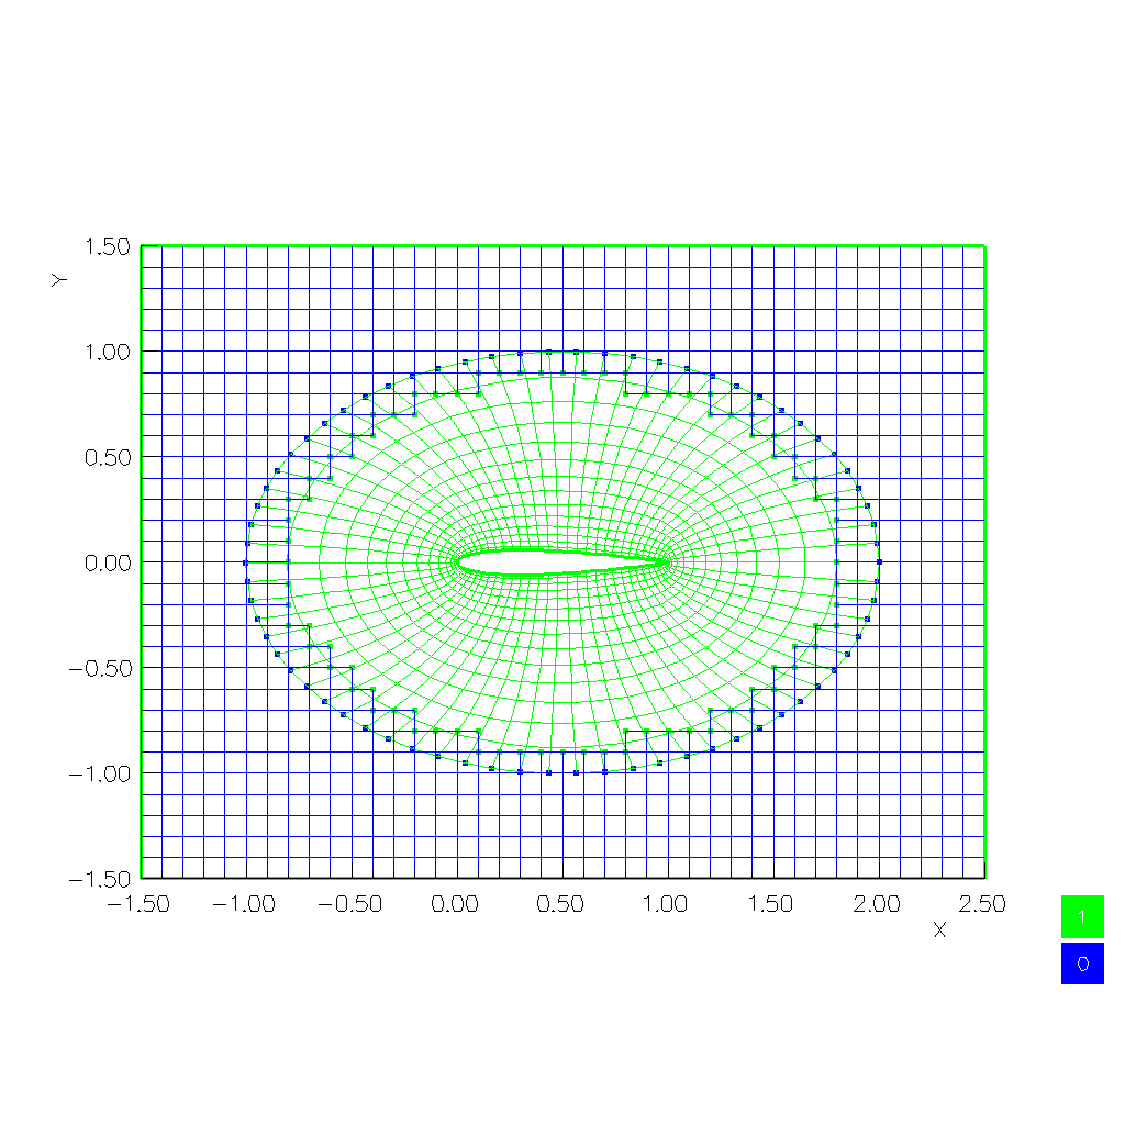
\includegraphics[height=6.0in]{\figures/naca0012}\\
  \caption{An overlapping grid for a NACA0012 airfoil}  \label{fig:naca0012}
  \end{center}
\end{figure}



% ------------------------------------------------------------------------------------------------------------
\clearpage
\subsection{Hybrid grid for the inlet-outlet}\index{hybrid grid}\index{unstructured grid}

The command file to create a hybrid for an inlet-outlet geometry is {\tt Overture\-/sampleGrids\-/inletOutlet.hyb.cmd}. 
%- \begin{multicols}{2}
%- {\footnotesize
%- \listinginput[1]{1}{\ogen /inletOutlet.hyb.cmd}
%- }
%-\end{multicols}

%- \begin{figure}[htb]
%-   \begin{center}
%-    % \epsfig{file=\figures/inletOutlet.hyb.ps,height=6.0in}
%-    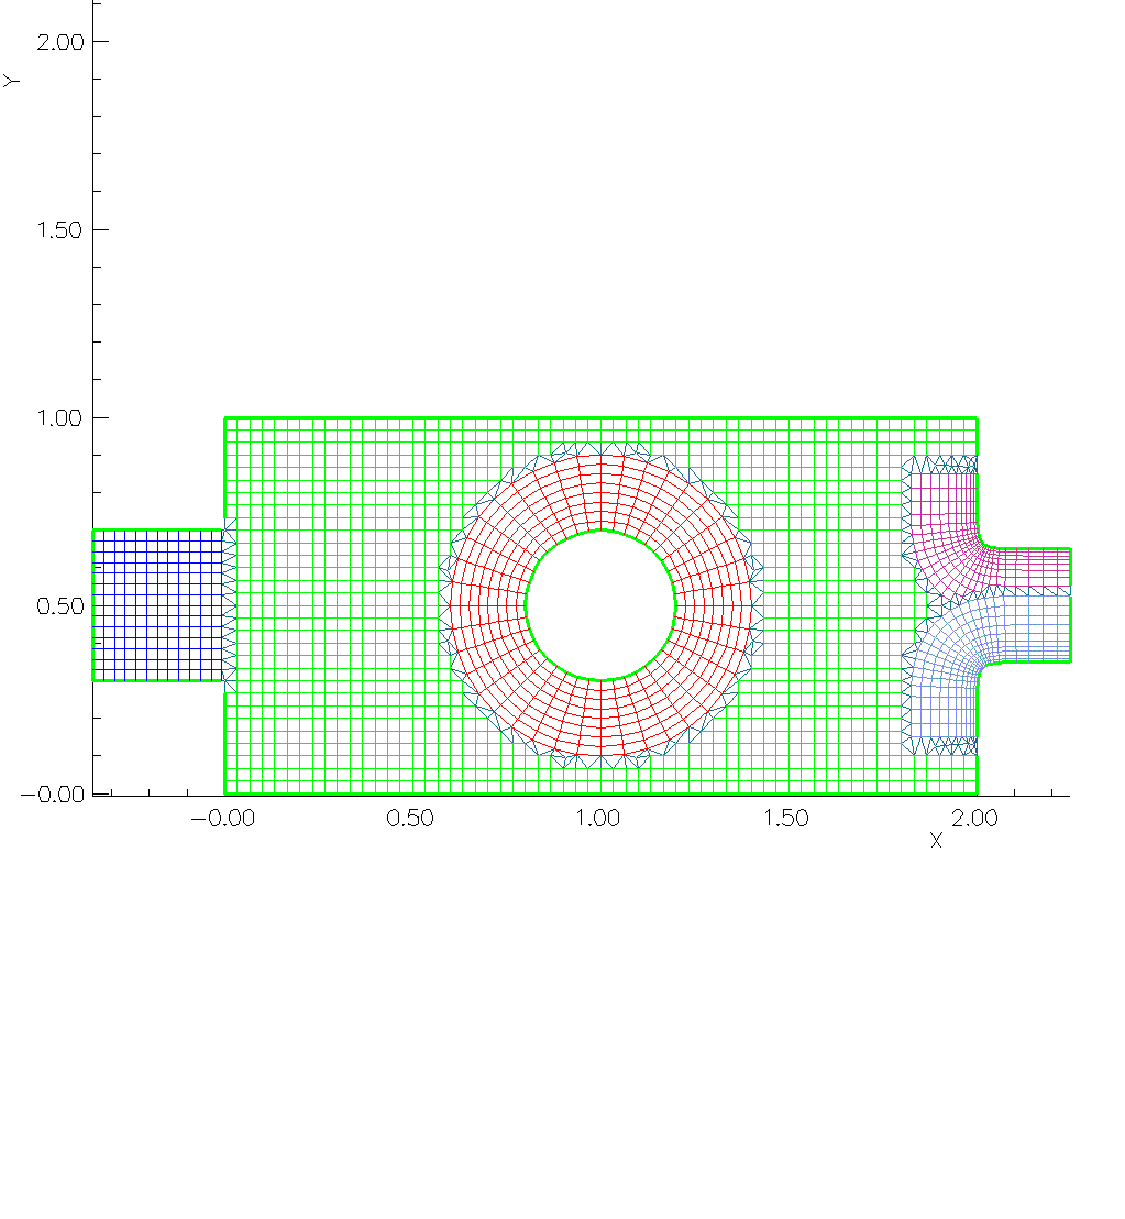
\includegraphics[height=6.0in]{\figures/inletOutlet_hyb}\\
%-   \caption{A hybrid grid for an inlet-outlet geometry.}
%-   \end{center}
%- \end{figure}
{
\newcommand{\figWidthd}{12cm}
\newcommand{\trimfig}[2]{\trimPlot{#1}{#2}{.0}{.0}{.325}{.35}}
\begin{figure}[hbt]
\begin{center}
\begin{tikzpicture}[scale=1]
  \useasboundingbox (0,.7) rectangle (12,5);  % set the bounding box (so we have less surrounding white space)
%
  \draw ( 0.0,0.) node[anchor=south west,xshift=-4pt,yshift=+0pt] {\trimfig{\figures/inletOutlet_hyb}{\figWidthd}};
%
 % \draw (current bounding box.south west) rectangle (current bounding box.north east);
% grid:
% \draw[step=1cm,gray] (0,0) grid (12,4);
\end{tikzpicture}
\end{center}
  \caption{A hybrid grid for an inlet-outlet geometry.}
\end{figure}
}


% \clearpage
\subsection{Stretched cube}

Here is a command file to create a simple box in 3D with stretched grid lines.
(file {\tt \sampleGrids/\-stretched\-Cube.cmd})
% {\footnotesize
% \listinginput[1]{1}{\ogen /stretchedCube.cmd}
% }
% The resulting grid is shown in figure~\ref{fig:stretchedCube}.
% \begin{figure}[htb]
%   \begin{center}
%    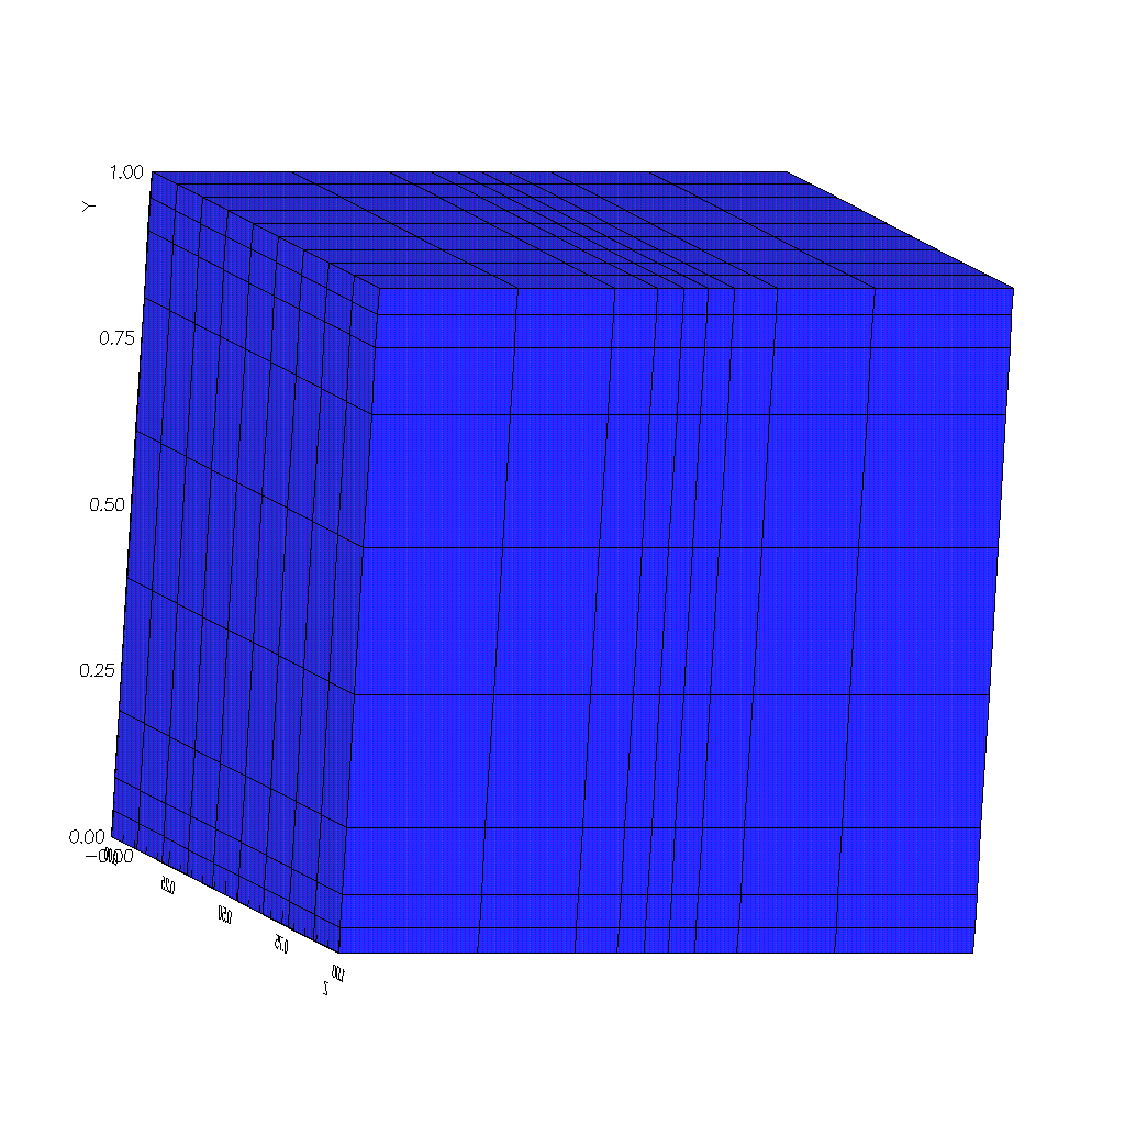
\epsfig{file=\figures/stretchedCube.ps,height=6.0in}
%   \caption{An overlapping grid for a stretched cube}  \label{fig:stretchedCube}
%   \end{center}
% \end{figure}

\noindent
\begin{minipage}{.4\linewidth}
{\footnotesize
\listinginput[1]{1}{\ogen //stretchedCube.cmd}
}
\end{minipage}\hfill
\begin{minipage}{.6\linewidth}
  \begin{center}
   % 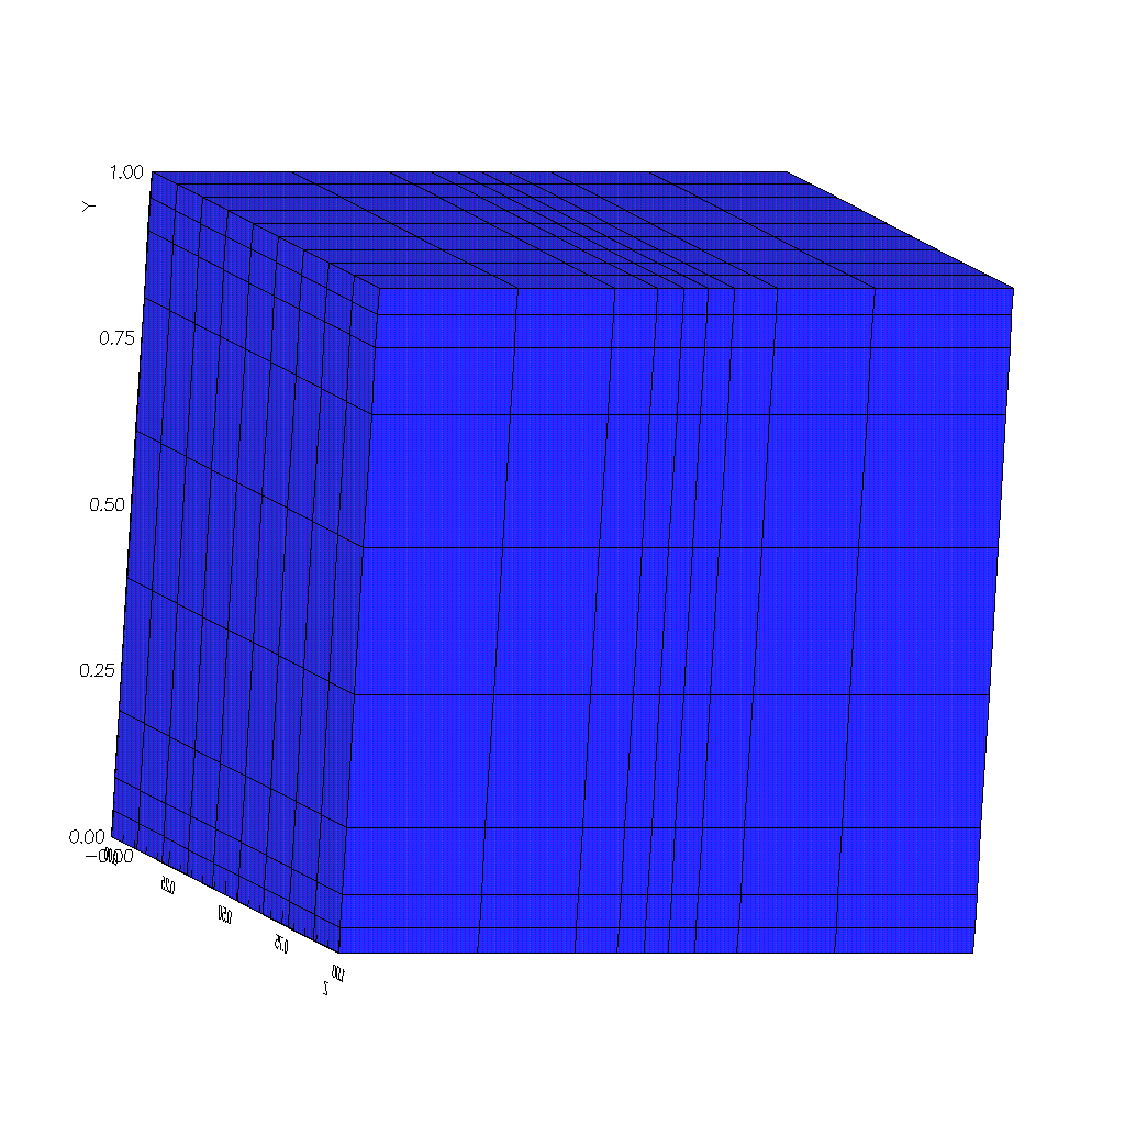
\epsfig{file=\figures/stretchedCube.ps,height=3.75in}  \\
   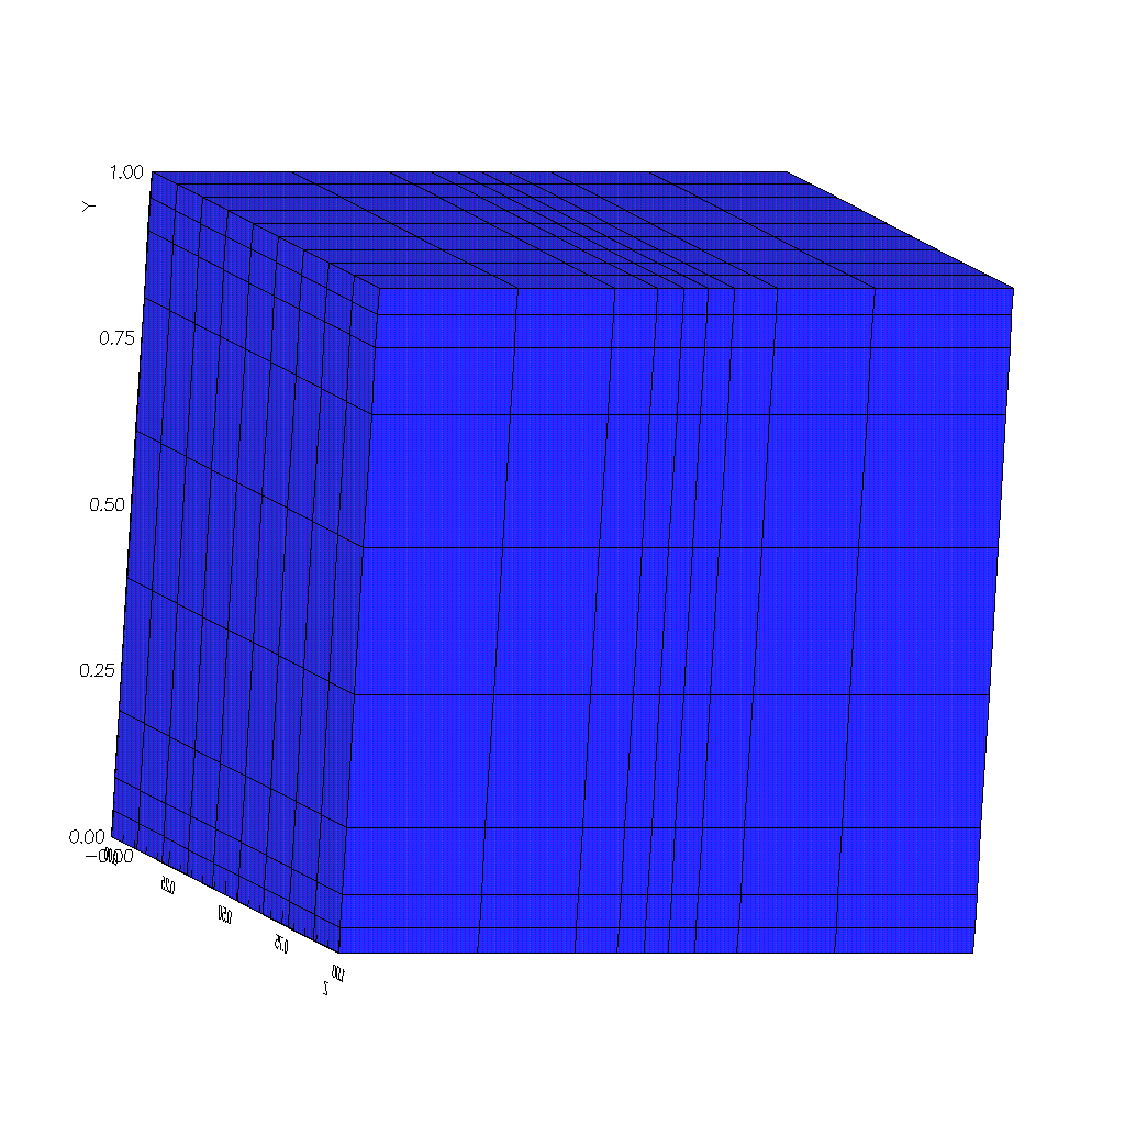
\includegraphics[height=3.75in]{\figures/stretchedCube}\\
  {An overlapping grid for a stretched cube.}  \label{fig:stretchedCube}
  \end{center}
\end{minipage}



\clearpage
\subsection{Sphere in a box}

Here is a command file to create a sphere in a box. The sphere is 
covered with two \Index{orthographic} patches, one for the north-pole and
one for the south-pole.
(file {\tt \sampleGrids/sib.cmd})
\begin{multicols}{2}
{\footnotesize
\listinginput[1]{1}{\ogen /sib.cmd}
}
\end{multicols}
The resulting grid is shown in figure~\ref{fig:sib}.
\begin{figure}[htb]
  \begin{center}
   %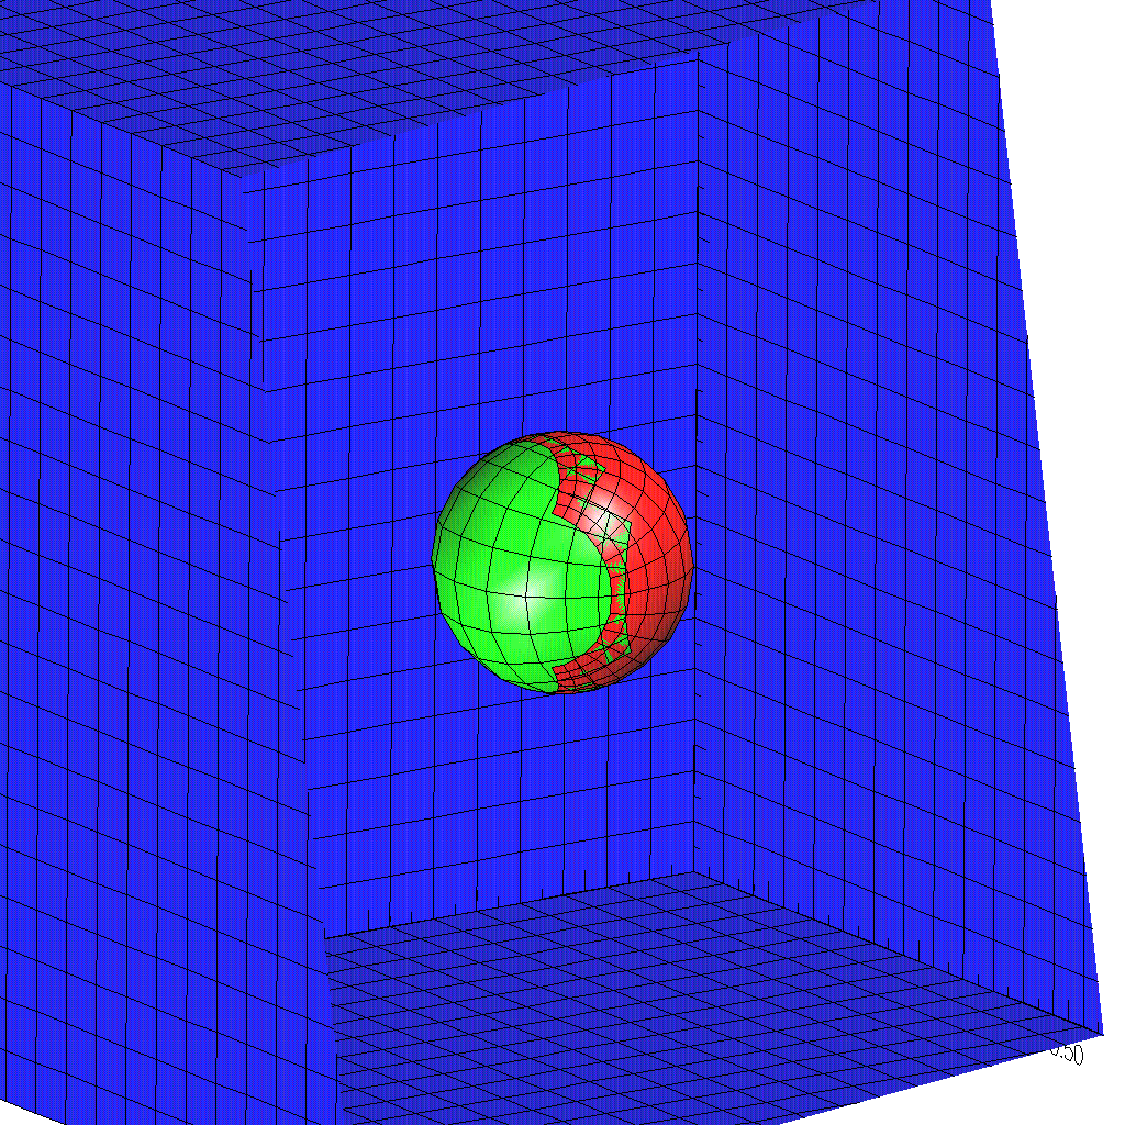
\epsfig{file=\figures/sib.ps,height=4.0in}
   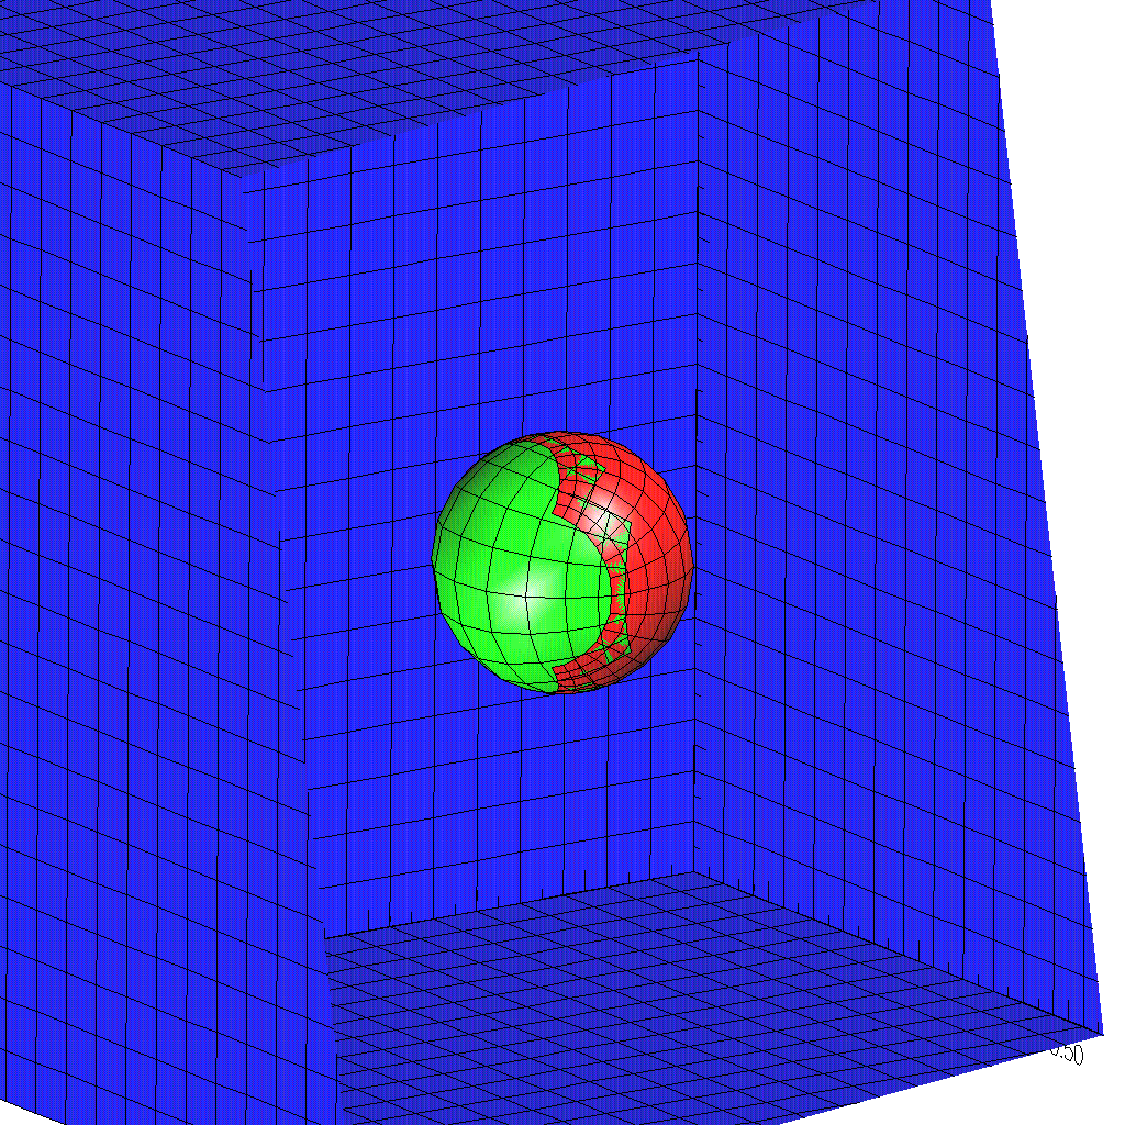
\includegraphics[height=4.0in]{\figures/sib}\\
  \caption{An overlapping grid for a sphere in a box. The sphere is covered
       with two patches.}  \label{fig:sib}
  \end{center}
\end{figure}
\begin{figure}[htb]
  \begin{center}
   % 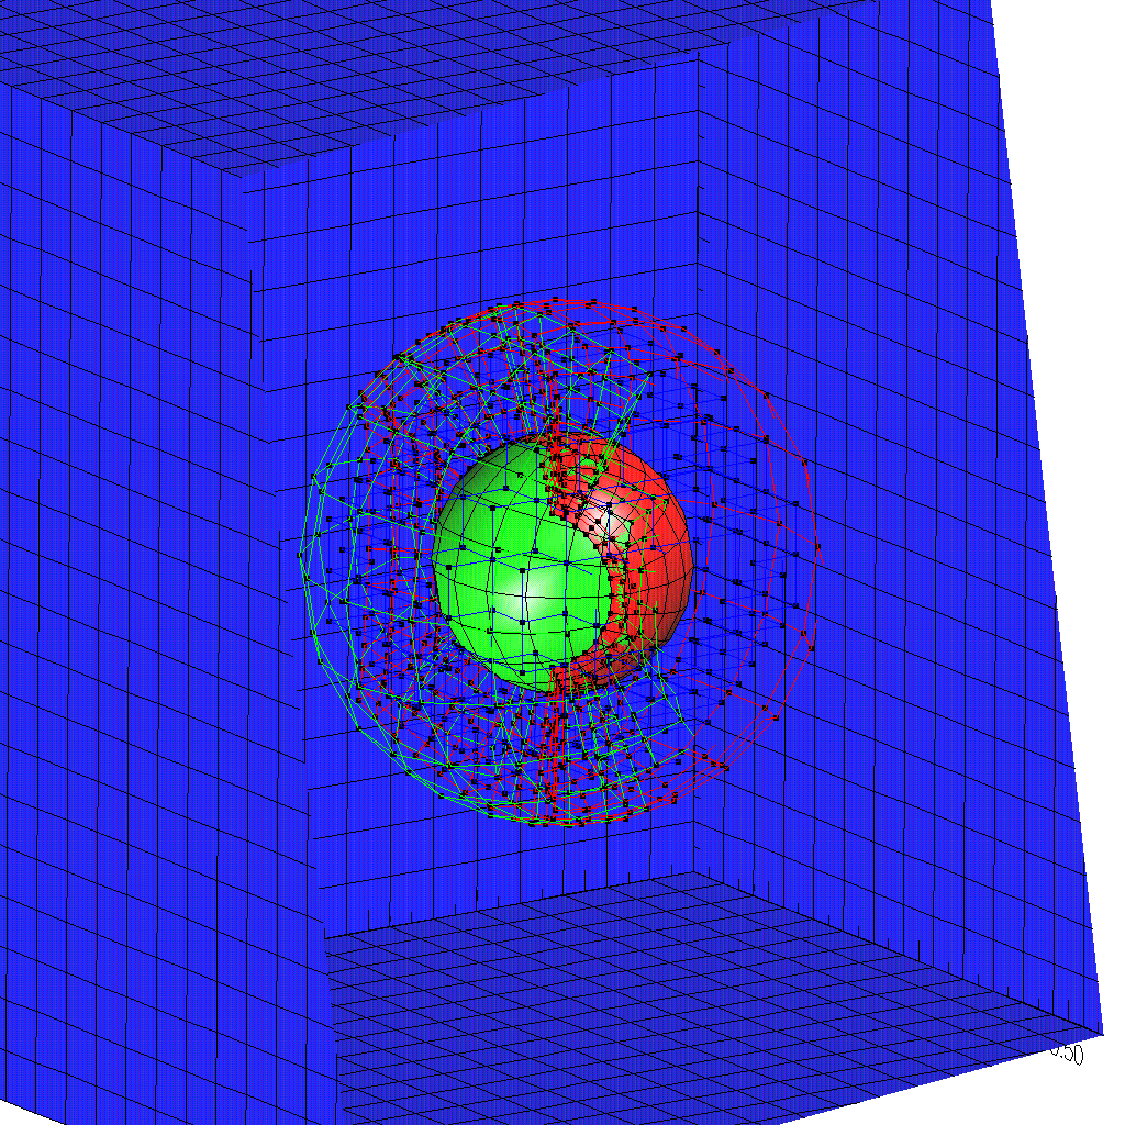
\epsfig{file=\figures/sib2.ps,height=4.0in}
   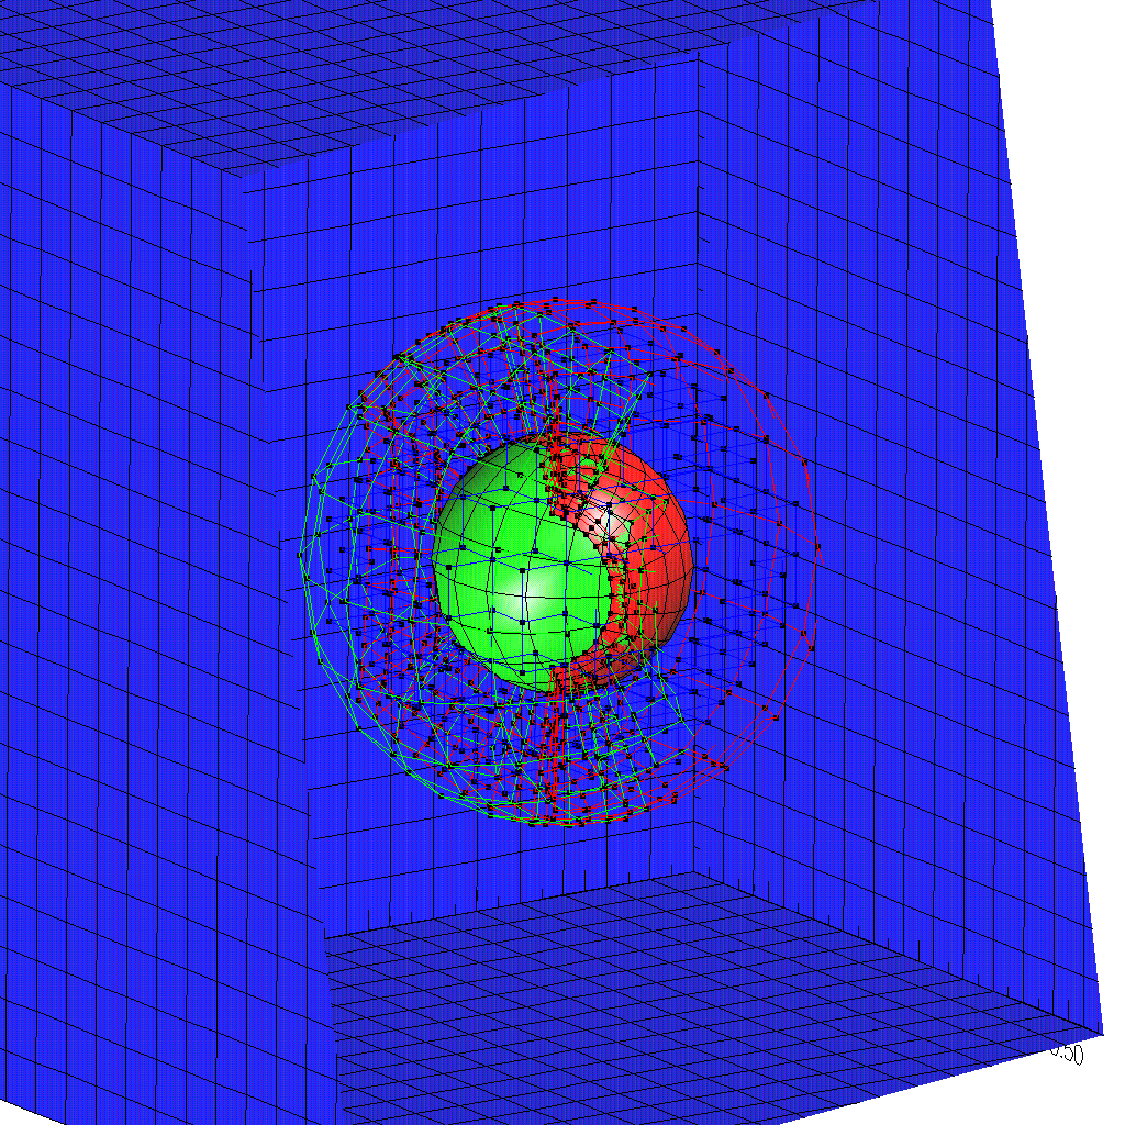
\includegraphics[height=4.0in]{\figures/sib2}
  \caption{An overlapping grid for a sphere in a box. The interpolation points are also shown.}
  \end{center}
\end{figure}
The cell-centered version can be made with {\tt \sampleGrids/sibCC.cmd}.


\clearpage
\subsection{Sphere in a tube}

Here is a command file to create a sphere in a cylindrical tube. The sphere is 
covered with two orthographic patches, one for the north-pole and
one for the south-pole. The sphere is contained in a tube that is represented
as a cylinderical annulus together with a rectangular box that forms the core
of the cylinder.
(file {\tt \sampleGrids/sphereInATube.cmd})
\begin{multicols}{2}
{\footnotesize
\listinginput[1]{1}{\ogen /sphereInATube.cmd}
}
\end{multicols}
The resulting grid is shown in figure~\ref{fig:sit}.
\begin{figure}[htb]
  \begin{center}
   % 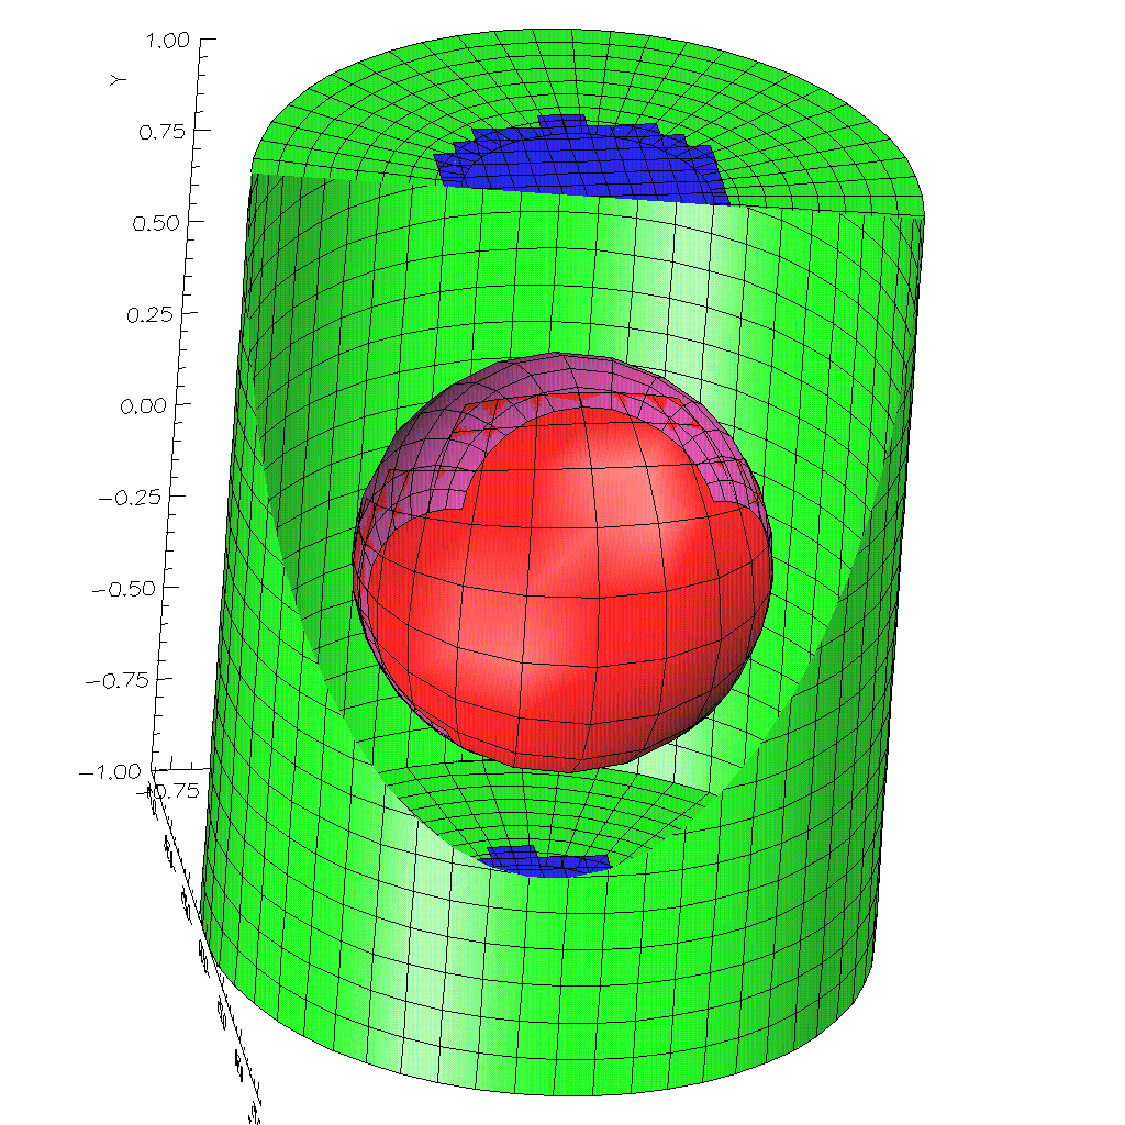
\epsfig{file=\figures/sit.ps,height=6.0in}
   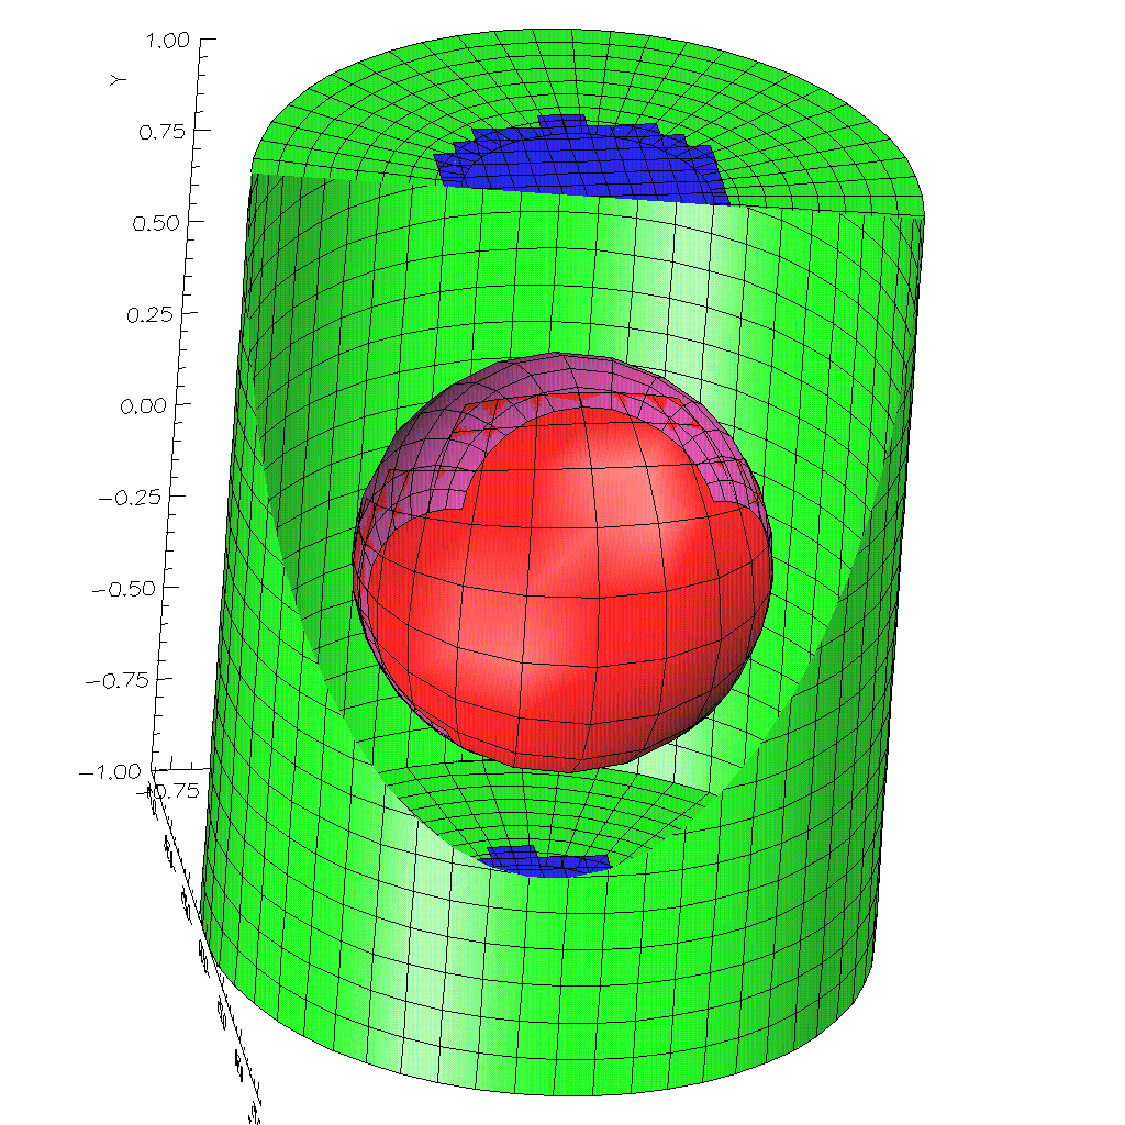
\includegraphics[height=6.0in]{\figures/sit}
  \caption{An overlapping grid for a sphere in a cylindrical tube}  \label{fig:sit}
  \end{center}
\end{figure}


\clearpage
\subsection{Intersecting pipes}

Here is a command file to create a grid for two intersecting pipes.
Each pipe is made from a cylindrical annulus with a rectangular grid for
the core. The pipes intersect using the poor man's intersection method
with non-conforming grids. (A more refined intersection would use a fillet).
The key point here is that the boundaries must not cut holes and so this
feature is turned off.
(file {\tt \sampleGrids/pipes.cmd})
\begin{multicols}{2}
{\footnotesize
\listinginput[1]{1}{\ogen /pipes.cmd}
}
\end{multicols}
The resulting grid is shown in figure~\ref{fig:pipes}.
\begin{figure}[htb]
  \begin{center}
   % 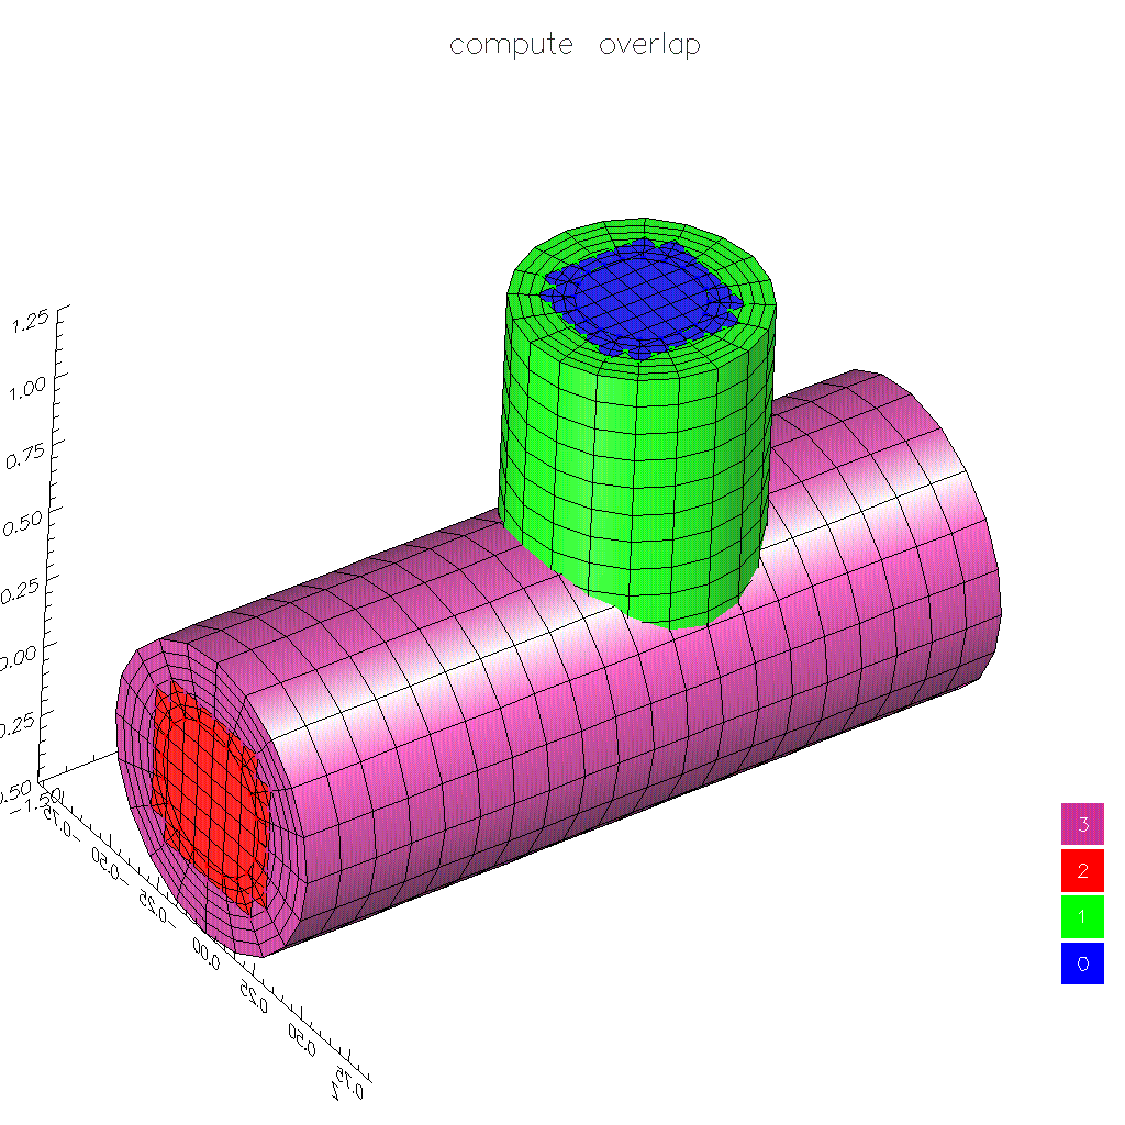
\epsfig{file=\figures/pipes.ps,height=6.0in}
   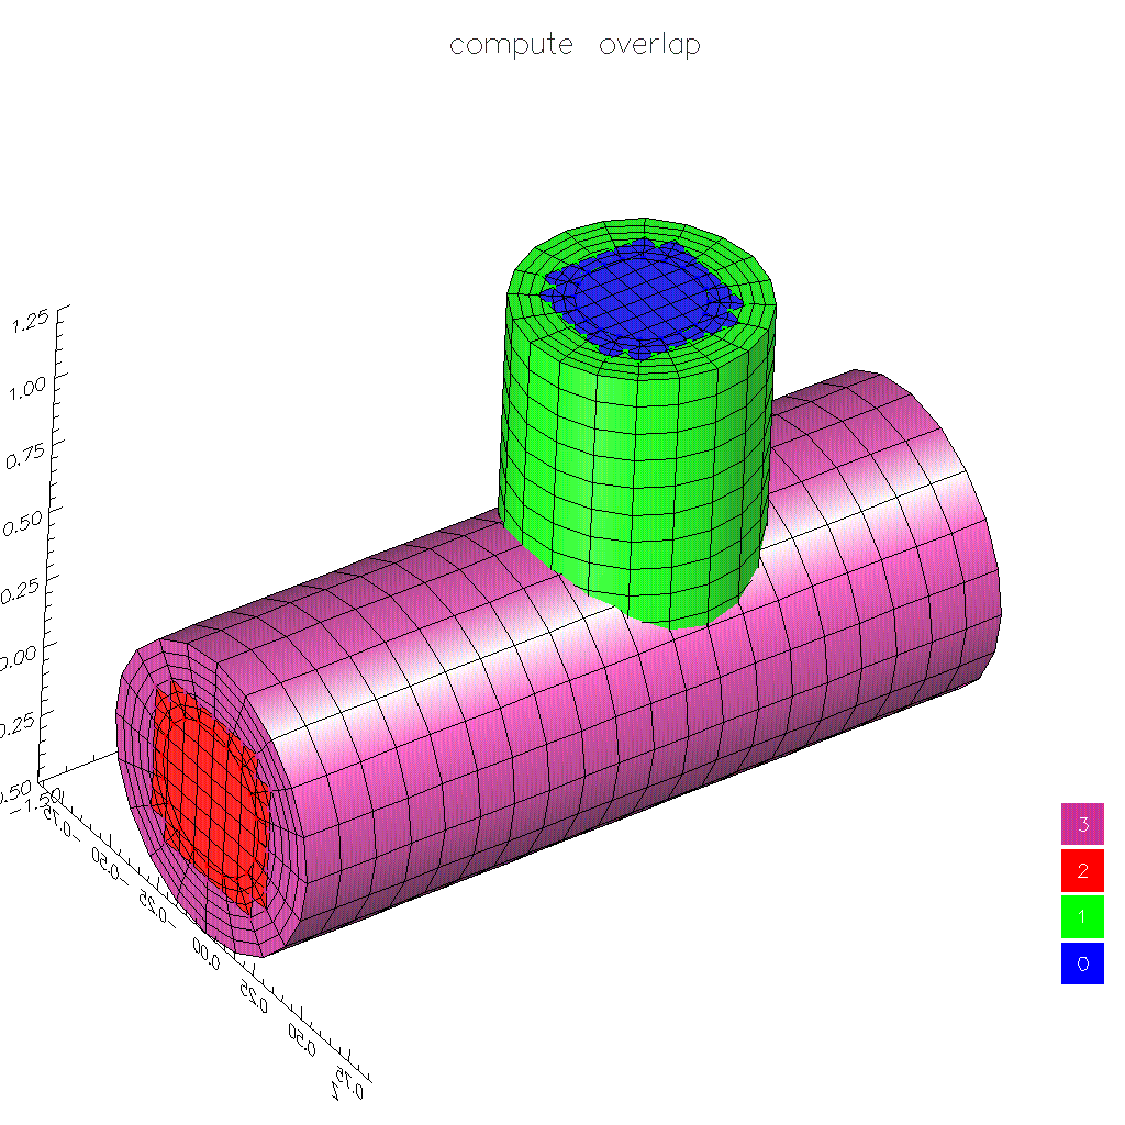
\includegraphics[height=6.0in]{\figures/pipes}
  \caption{An overlapping grid for two intersecting pipes}  \label{fig:pipes}
  \end{center}
\end{figure}

\clearpage
\subsection{Body Of Revolution}

Here is a command file to create a grid for a \Index{body of revolution}.
The body of revolution is created by revolving a two-dimensional grid about a given line.
The two dimensional grid in this case is created with the {\tt SmoothedPolygon}
Mapping.
The body of revolution has a spherical polar singularity at both ends. We generate a
new Mapping to cover each singularity. We reparameterize the ends using an orthographic
transformation.
(file {\tt \sampleGrids/revolve.cmd})
\begin{multicols}{2}
{\footnotesize
\listinginput[1]{1}{\ogen /revolve.cmd}
}
\end{multicols}
The resulting grid is shown in figure~\ref{fig:revolve}.
\begin{figure}[htb]
  \begin{center}
   % 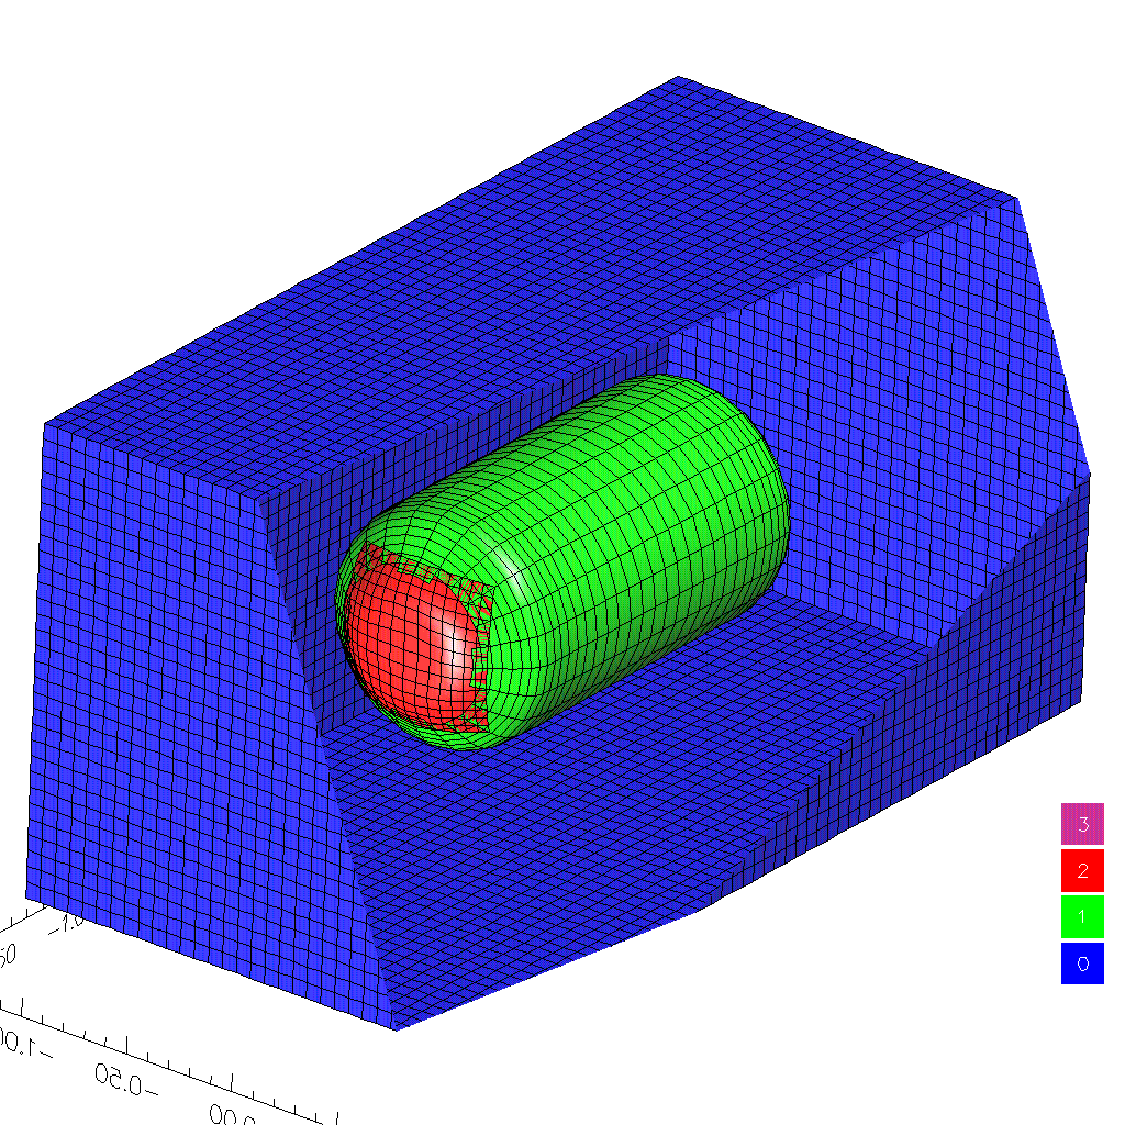
\epsfig{file=\figures/revolve.ps,height=6.0in}
   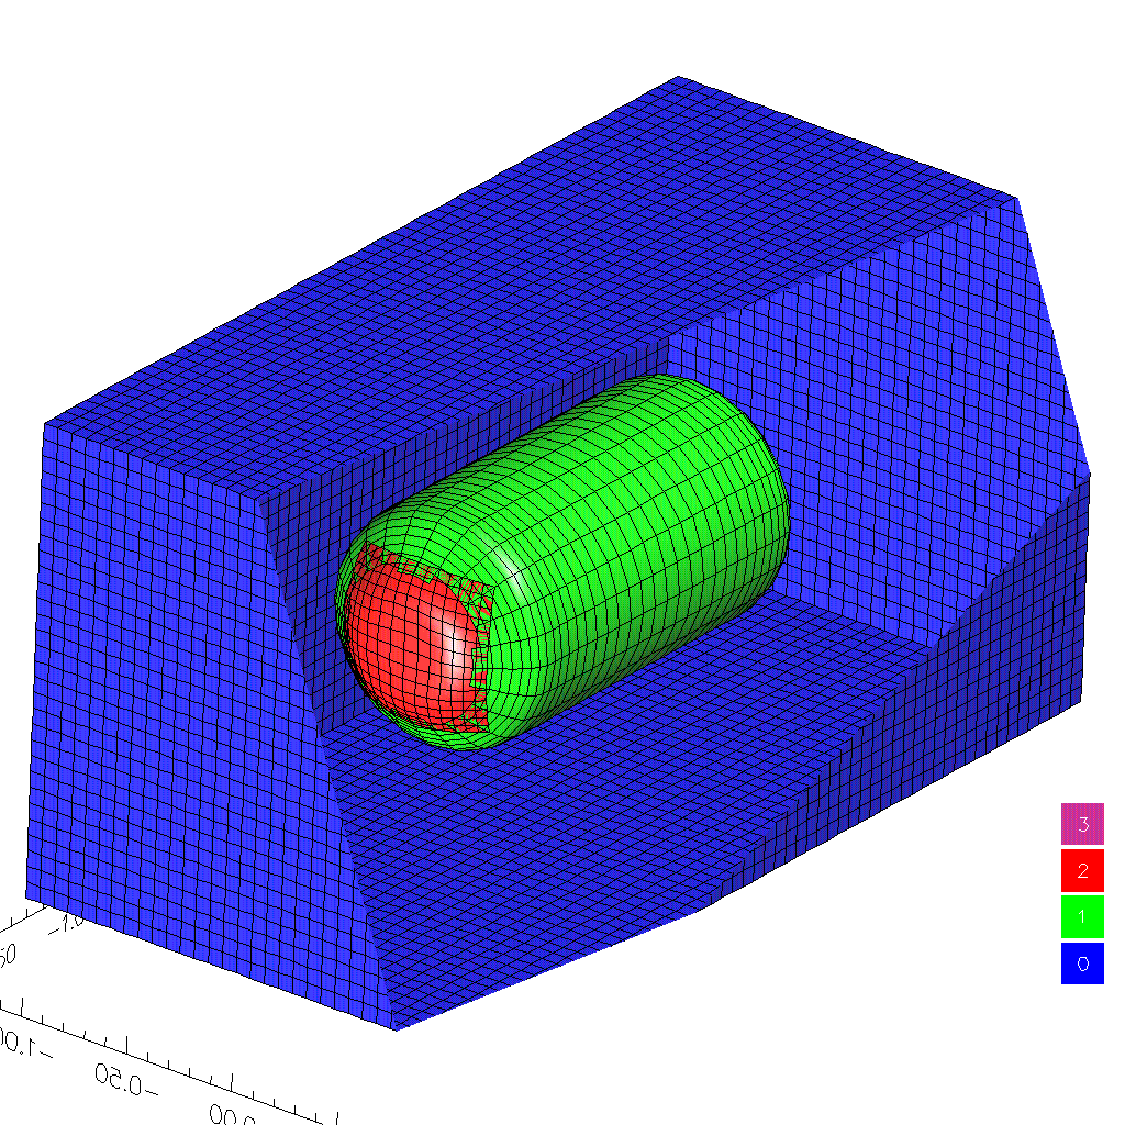
\includegraphics[height=6.0in]{\figures/revolve}
  \caption{An overlapping grid for a body of revolution. The body is generated by revolving 
   a two-dimensional smoothed-polygon mapping. Orthographic patches are used to cover the
    singularities at the ends of the body.}  \label{fig:revolve}
  \end{center}
\end{figure}



\clearpage
\subsection{3D valve}

Here is a command file to create a grid for a three dimensional valve. The cross-section
of this geometry is similar to the two-dimensional valve shown earlier.
(file {\tt \sampleGrids/valve3d.cmd})
\begin{multicols}{2}
{\footnotesize
\listinginput[1]{1}{\ogen /valve3d.cmd}
}
\end{multicols}
The resulting grid is shown in figure~\ref{fig:valve3d}.
\begin{figure}[htb]
  \begin{center}
   % 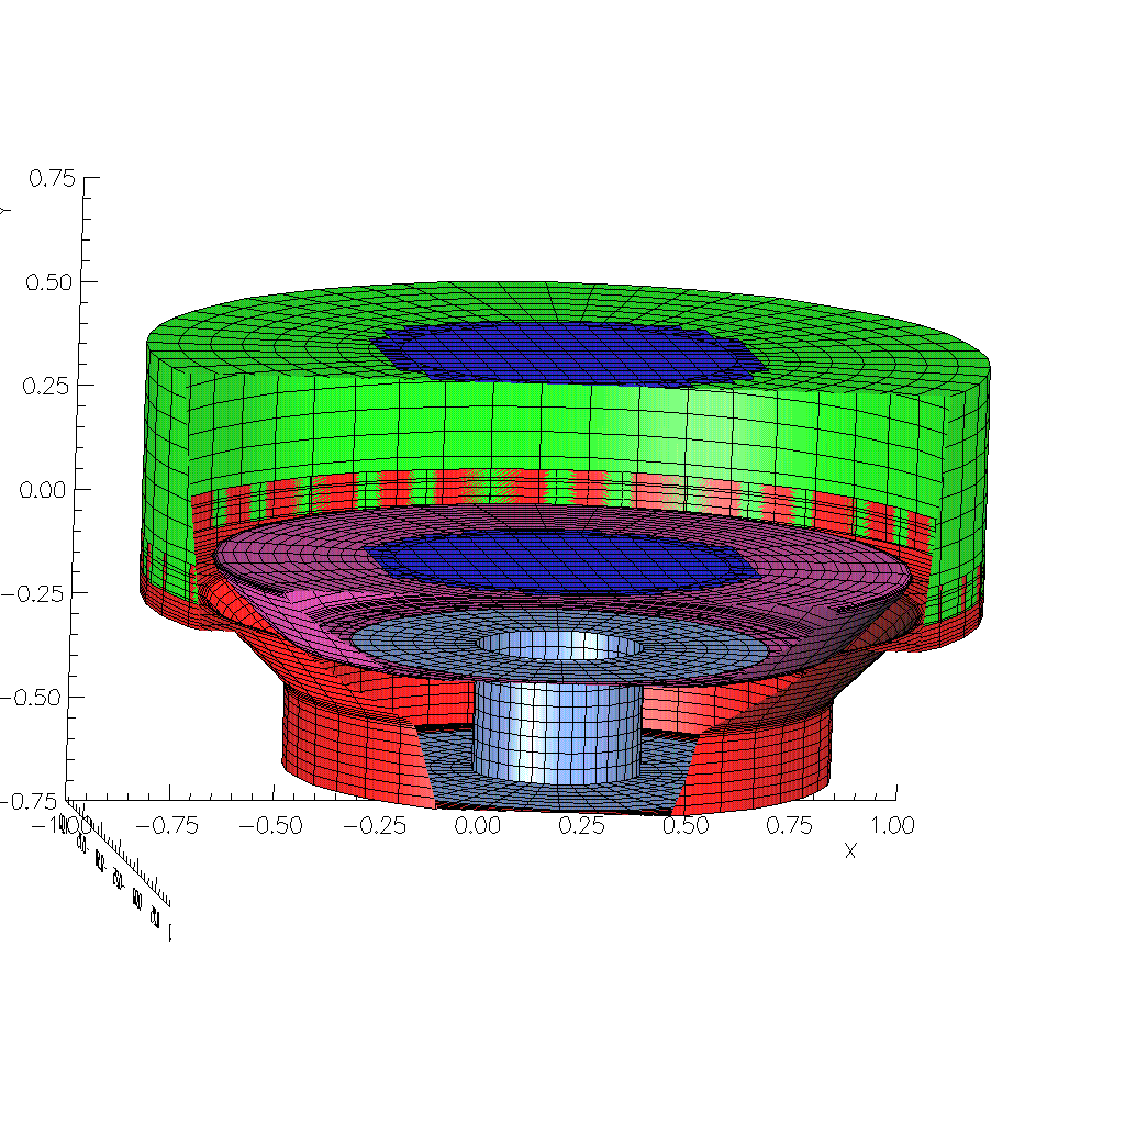
\epsfig{file=\figures/valve3d.ps,height=6.0in}
   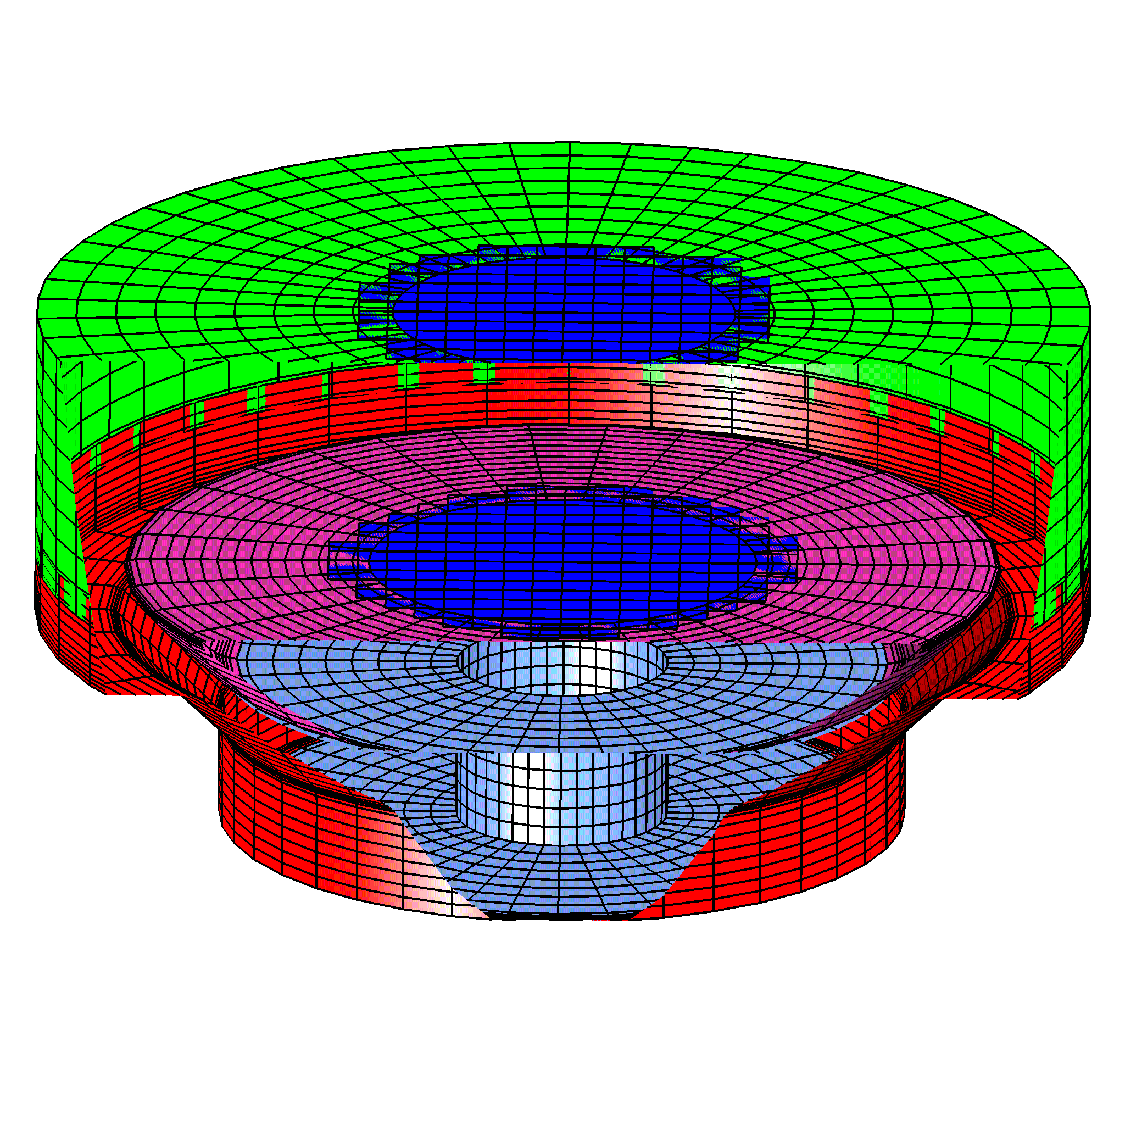
\includegraphics[height=6.0in]{\figures/valve3dGrid}
  \caption{An overlapping grid for a three-dimensional valve. } \label{fig:valve3d}
  \end{center}
\end{figure}

% ----------------------------------------------------------------------------------------------
\clearpage
\subsection{3D wing in a box}\label{sec:3dWingInABox}

The command file {\tt Overture/sampleGrids/wing3d.cmd} shows how to build a grid 
for a three-dimensional wing in a box. The wing is defined as a set of cross-section curves (ellipses in
this case)
that are used with the CrossSectionMapping. The CrossSectionMapping has an option to 
close off the start and/or end of the surface by transitioning the cross-sections
so they converge to a point. The orthographic transform is used to create cap grids on
the tips of the wing. These grids work best when the cross-sections near the tips are
nearly ellipses. Otherwise the cap grids may have poor quality cells. In the latter case
one could use the hyperbolic grid generator to construct a better quality grid for
the cap (see Section~\ref{sec:JoukowskyWing3d}). 

{
\newcommand{\figWidthd}{7cm}
\newcommand{\trimfig}[2]{\trimPlot{#1}{#2}{.0}{.0}{.15}{.15}}
\begin{figure}[hbt]
\begin{center}
\begin{tikzpicture}[scale=1]
  \useasboundingbox (0,.5) rectangle (7.,4.75);  % set the bounding box (so we have less surrounding white space)
%
  \draw ( 0.0,0.) node[anchor=south west,xshift=-4pt,yshift=+0pt] {\trimfig{\figures/wing3dGrid}{\figWidthd}};
%
 % \draw (current bounding box.south west) rectangle (current bounding box.north east);
% grid:
%  \draw[step=1cm,gray] (0,0) grid (9,4);
\end{tikzpicture}
\end{center}
\caption{An overlapping grid for a three-dimensional wing in a box. } \label{fig:wing3d}
\end{figure}
}

%- {
%- \begin{figure}[htb]
%-   \begin{center}
%-    % 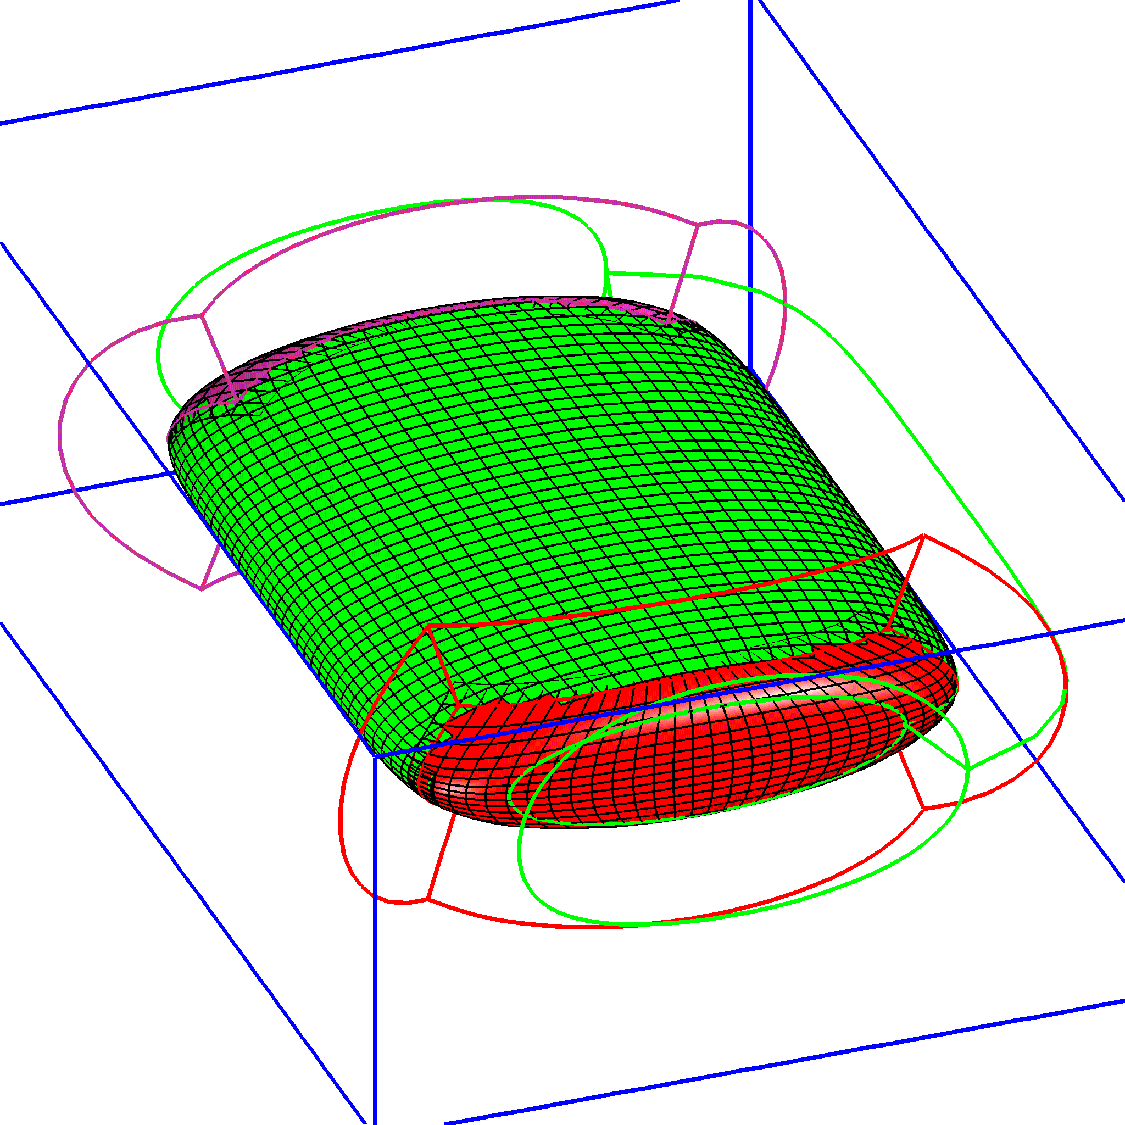
\epsfig{file=\figures/wing3dGrid.ps,height=6.0in}
%-    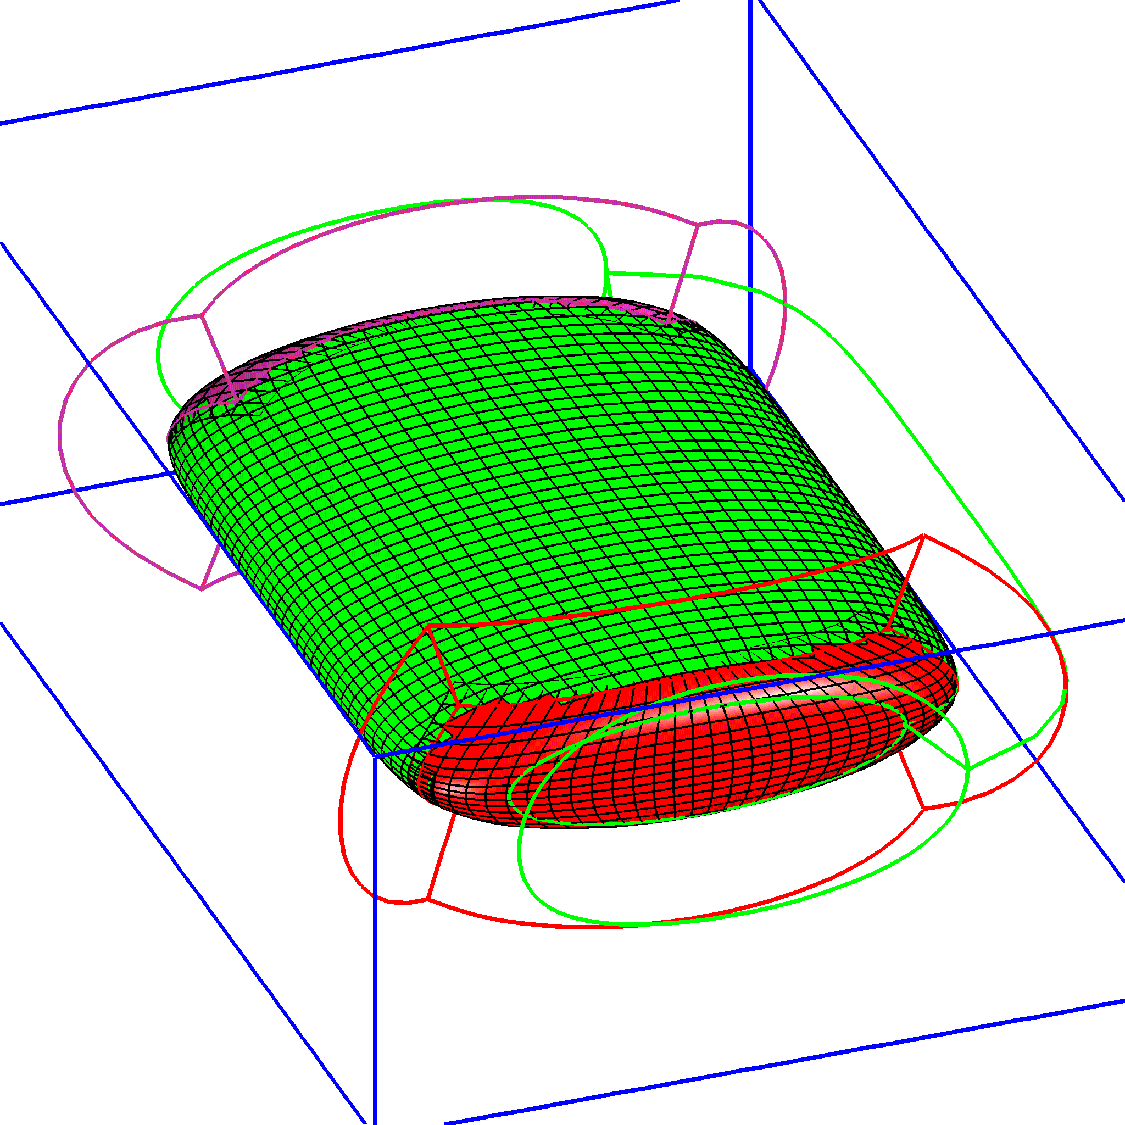
\includegraphics[height=7cm]{\figures/wing3dGrid}
%-   \caption{An overlapping grid for a three-dimensional wing in a box. } \label{fig:wing3d}
%-   \end{center}
%- \end{figure}
%- }

% ----------------------------------------------------------------------------------------------
% \clearpage
\subsection{3D wing with Joukowsky cross-sections}\label{sec:JoukowskyWing3d}

The command file {\tt Overture/sampleGrids/wingj.cmd} shows another way to build a grid 
for a three-dimensional wing. The wing surface is defined as a Nurbs with the points
on the cross sections generated directly in the command file using perl. 

\noindent{\bf Notes:}
\begin{enumerate}
  \item The wing surface is defined by Joukowsky cross-sections.
  \item The tip is rounded with the cross-sections changing into an ellipse and converging to a point. 
  \item The main wing grid is generated by removing the region near the singular tip.
  \item A hyperbolic grid is grown over the tip region. We cannot use the original wing surface for growing
        this tip grid
        since the surface is not connected across the singular point (and the hyperbolic grid generator
        would get confused). Therefore we split the wing surface in the region of the tip into two
        separate surfaces and then construct a CompositeSurface and global triangulation for these
        two patches. We can then grow the tip grid on this CompositeSurface. 
\end{enumerate}

{
\newcommand{\figWidthd}{8cm}
\newcommand{\trimfig}[2]{\trimPlot{#1}{#2}{.0}{.0}{.25}{.23}}
\begin{figure}[hbt]
\begin{center}
\begin{tikzpicture}[scale=1]
  \useasboundingbox (0,.5) rectangle (9.,4.);  % set the bounding box (so we have less surrounding white space)
%
  \draw ( 0.0,0.) node[anchor=south west,xshift=-4pt,yshift=+0pt] {\trimfig{\figures/wingjGrid}{\figWidthd}};
%
 % \draw (current bounding box.south west) rectangle (current bounding box.north east);
% grid:
%  \draw[step=1cm,gray] (0,0) grid (9,4);
\end{tikzpicture}
\end{center}
  \caption{An overlapping grid for a three-dimensional wing with Joukowsky cross-sections and
       a rounded tip. } \label{fig:JoukowskyWing3d}
\end{figure}
}

%- \begin{figure}[htb]
%-   \begin{center}
%-   % 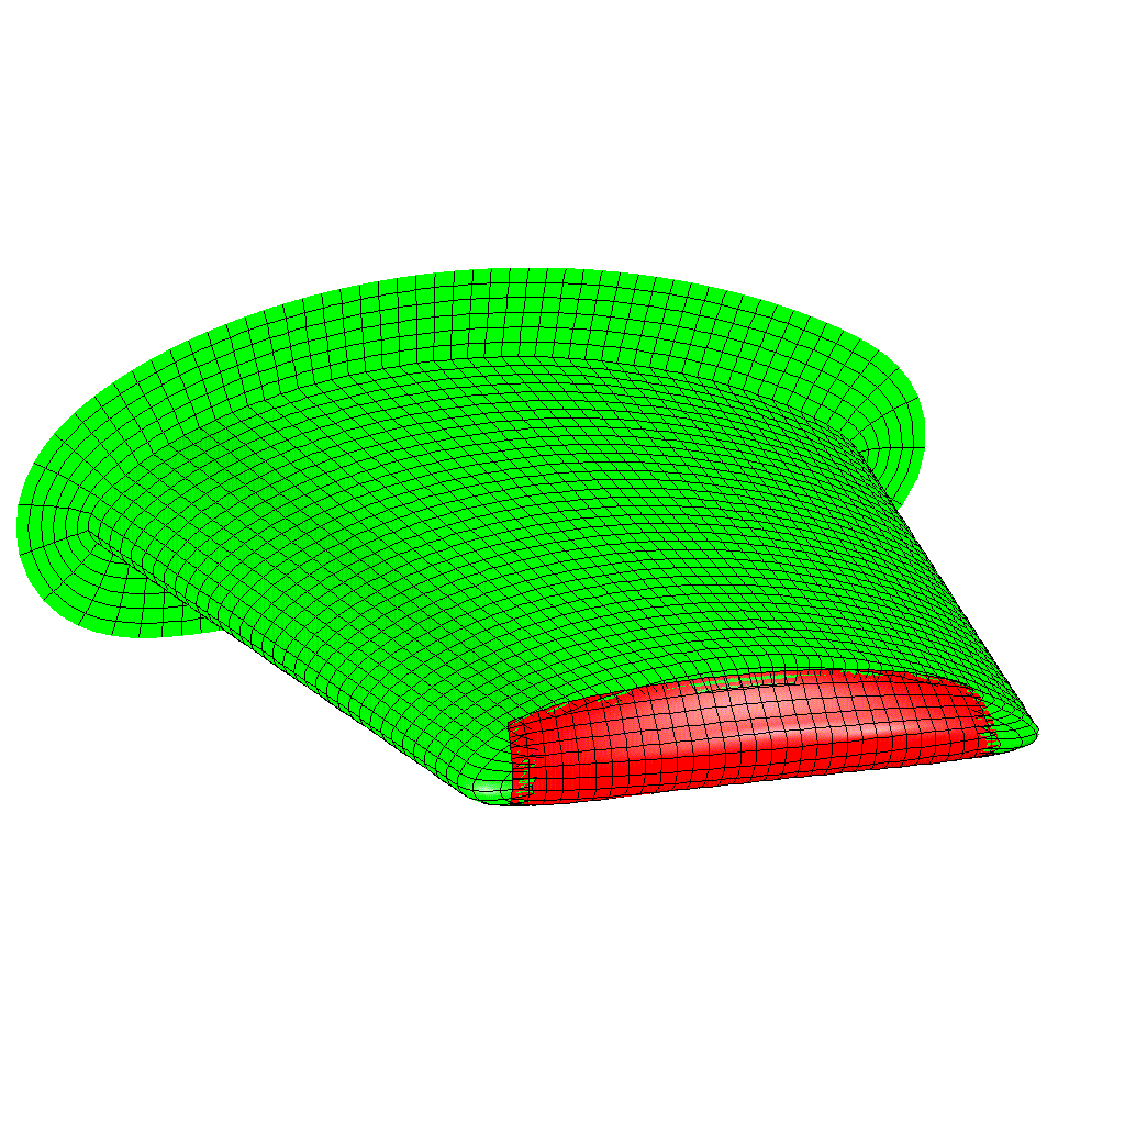
\epsfig{file=\figures/wingjGrid.ps,height=6.0in}
%-    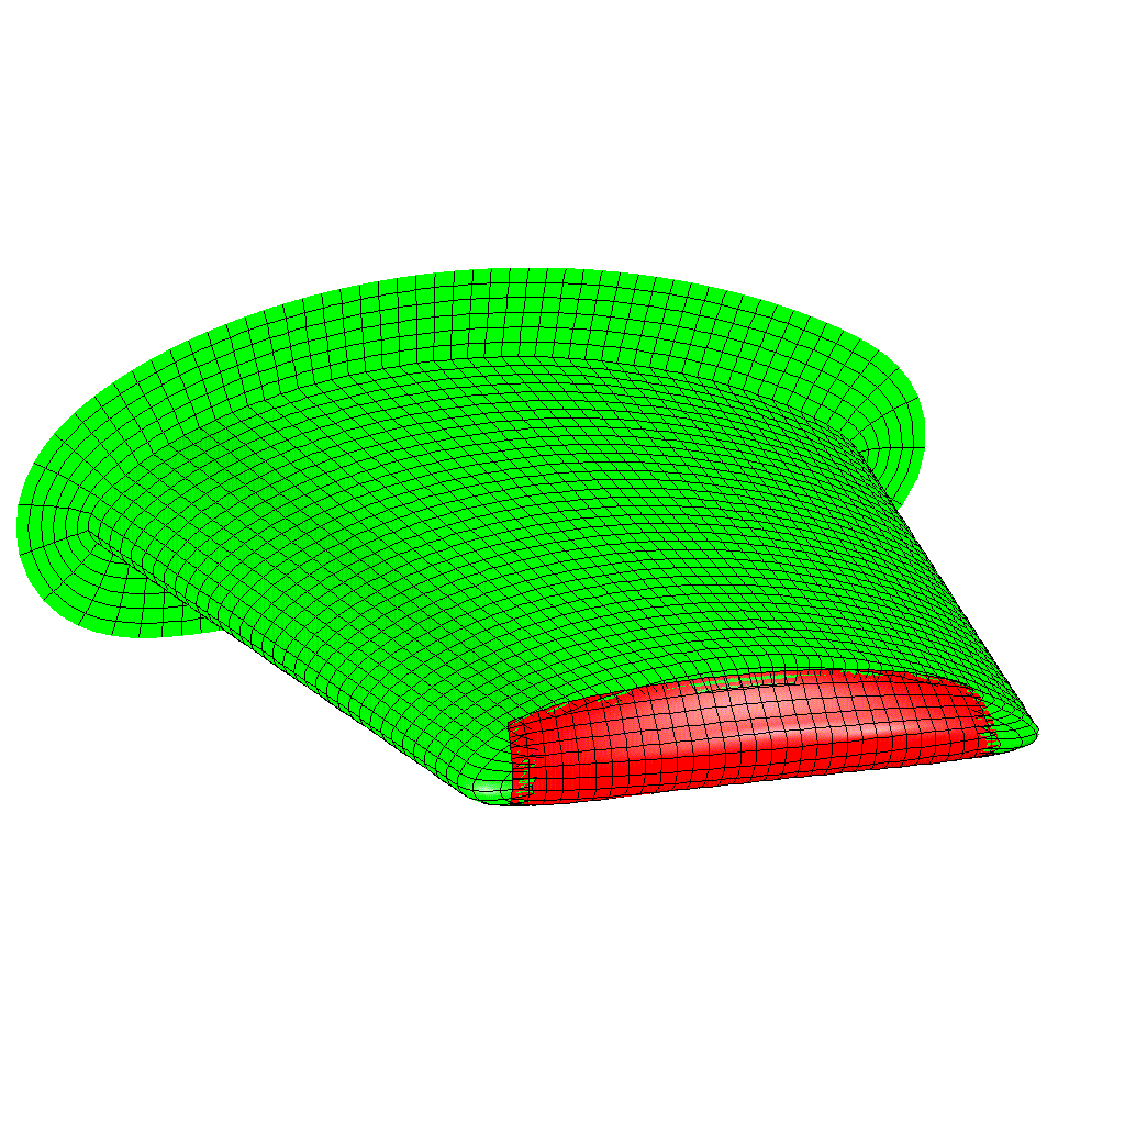
\includegraphics[height=6.0in]{\figures/wingjGrid}
%-   \caption{An overlapping grid for a three-dimensional wing with Joukowsky cross-sections and
%-        a rounded tip. } \label{fig:JoukowskyWing3d}
%-   \end{center}
%- \end{figure}


% ----------------------------------------------------------------------------------------------
\clearpage
\subsection{Three-dimensional flat-plate wing}\label{sec:FlatPlateWing}

The command file {\tt Overture/sampleGrids/flatPlateWingGrid.cmd} shows how to build a grid 
for a three-dimensional {\em flat-plate} wing in a box. The wing is defined as a set of 
cross-section curves (defined from a SmoothedPolygon)
that are used with the CrossSectionMapping. The CrossSectionMapping has an option to 
close off the start and/or end of the surface by transitioning the cross-sections
so they converge to a point. The orthographic transform is used to create intermediate cap grids on
the tips of the wing. Since these cap grids have poor quaility cells, the hyperbolic grid generator
is used to define new grids over the tips. The hyperbolic surface grids are generated on the orthographic patches (which still
accurately define the surface).

\begin{figure}[htb]
  \begin{center}
   % 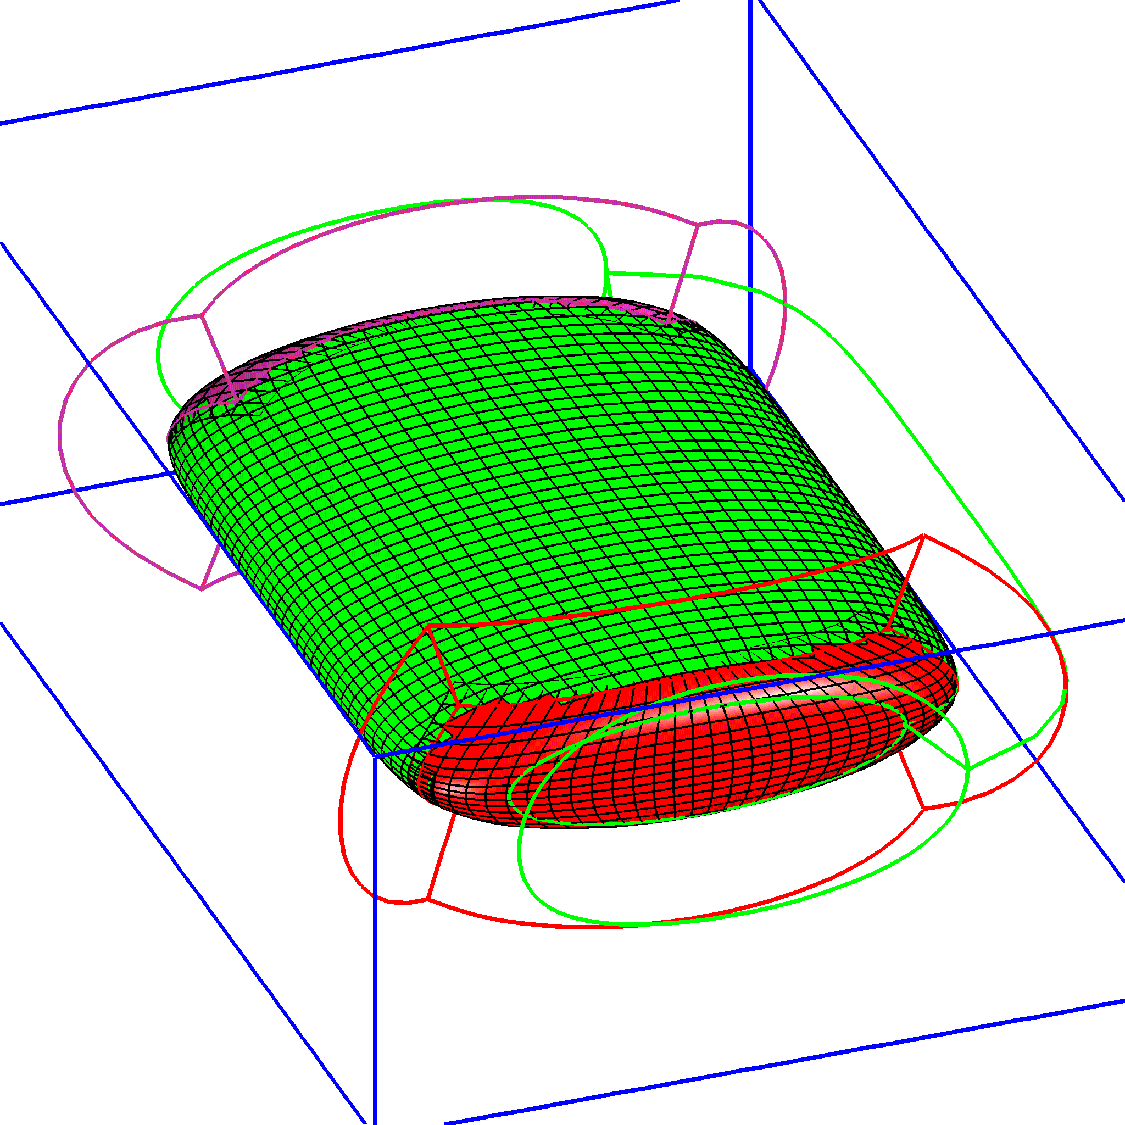
\epsfig{file=\figures/wing3dGrid.ps,height=6.0in}
   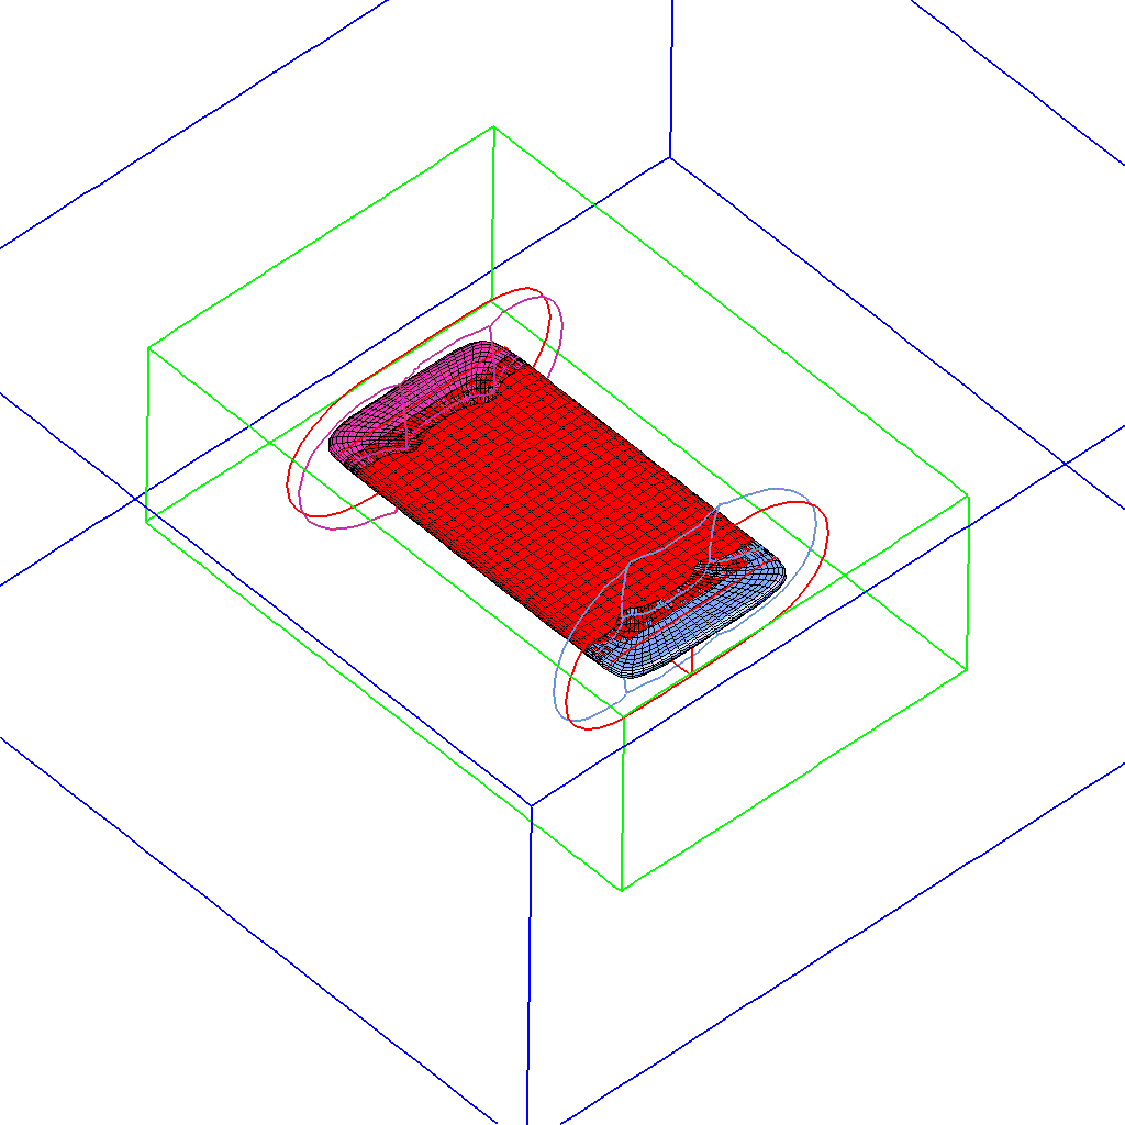
\includegraphics[height=7cm]{\figures/flatPlateWingGrid}
   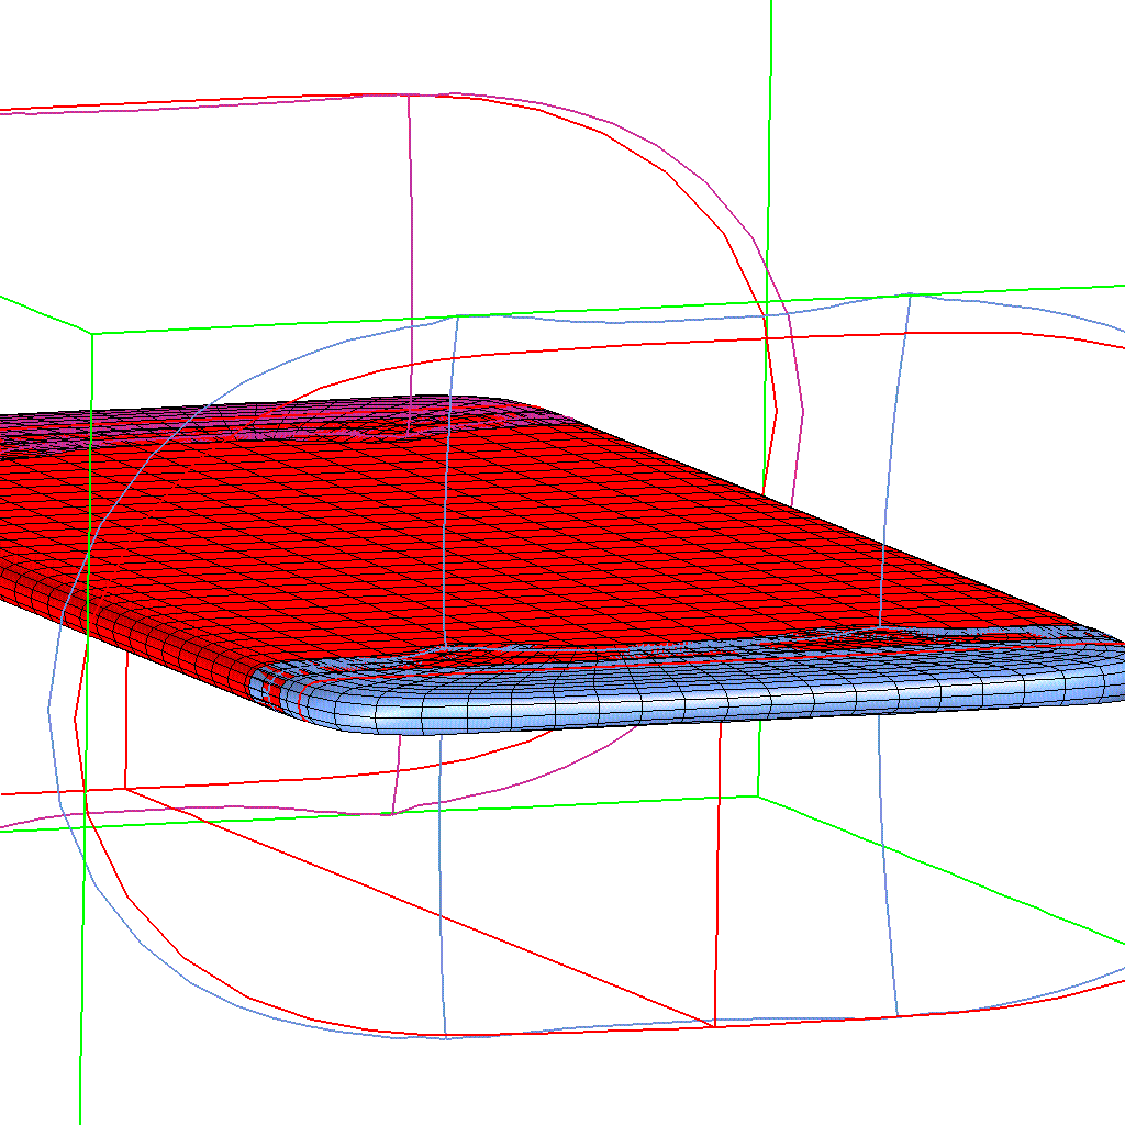
\includegraphics[height=7cm]{\figures/flatPlateWingGridCloseup}
  \caption{An overlapping grid for a three-dimensional flat-plate wing in a box. } \label{fig:flatPlateWingGrid}
  \end{center}
\end{figure}


% ----------------------------------------------------------------------------------------------
\subsection{Lofted box}\label{sec:LoftedBox}

The command file {\tt Overture/sampleGrids/loftedBox.cmd} constructs a grid for
the region exterior to a box (cube) with slightly rounded corners. 
The LoftedSurface Mapping is used to define the surface. See the mapping documentation
for further details on the LoftedSurface Mapping.

\begin{figure}[htb]
  \begin{center}
   % 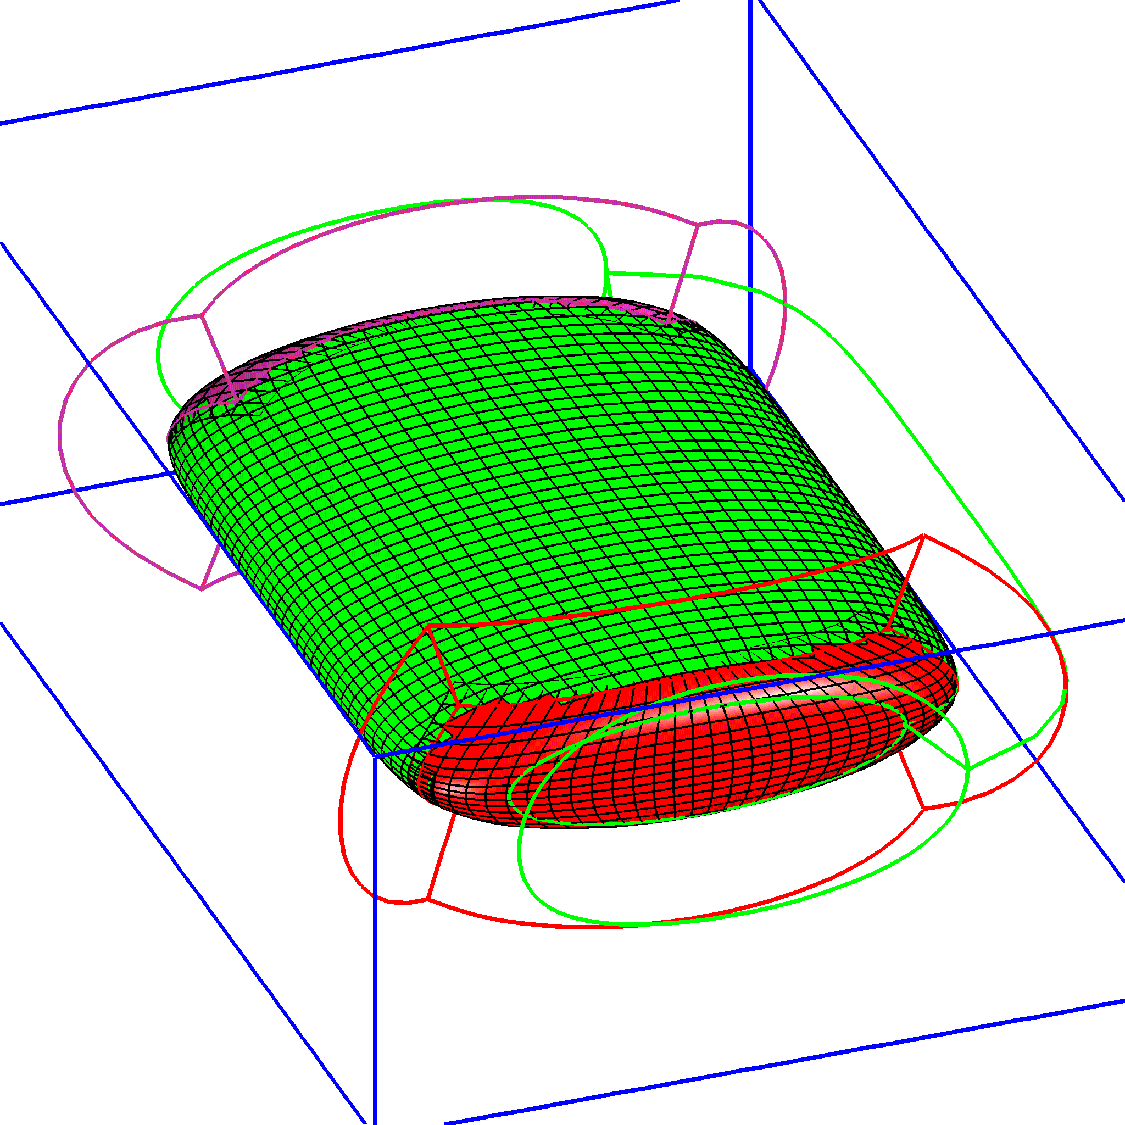
\epsfig{file=\figures/wing3dGrid.ps,height=6.0in}
   \includegraphics[height=7cm]{\figures/loftedBoxGrid}
  \caption{An overlapping grid for the region exterior to a box constructed with the LoftedSurface Mapping. } \label{fig:loftedBoxGrid}
  \end{center}
\end{figure}



% ----------------------------------------------------------------------------------------------
\subsection{Lofted Joukowsky Wing}\label{sec:LoftedJoukowskyWing}

The command file {\tt Overture/sampleGrids/loftedJoukowskyFlatTip.cmd} constructs a grid for
a wing with cross-sections defined as Joukoswky airfoils and a {\em flat} tip. The surface
was defined by the LoftedSurface Mapping~\cite{MAPPINGS}. The LoftedSurface Mapping was used to add a
twist to the wing and also to add flattened tip.

\begin{figure}[htb]
  \begin{center}
   % \epsfig{file=\figures/wing3dGrid.ps,height=6.0in}
   \includegraphics[height=10cm]{\figures/loftedJoukowskyFlatTipGrid}
  \caption{An overlapping grid for a wing with a Joukoswky airfoil and a {\em flat} tip
            constructed with the LoftedSurface Mapping. } \label{fig:loftedJoukowskyWing}
  \end{center}
\end{figure}

% ----------------------------------------------------------------------------------------------
\subsection{Lofted Wigley Ship Hull}\label{sec:LoftedWigleyShipHull}

The command file {\tt Overture/sampleGrids/loftedShipHullGrid.cmd} constructs a grid for
a Wigley ship hull as shown in Figure~\ref{fig:loftedShipHullGrid}. The surface
is defined by the LoftedSurface Mapping, see the description in~\cite{MAPPINGS}. 

The basic steps to construct the grid for the Wigley hull are
\begin{enumerate}
  \item Build the lofted surface for the ship hull.
  \item Create an orthographic patch on the bow (and stern) to remove the spherical polar coordinate singularity 
          (see Figure~\ref{fig:loftedShipHullGrid}).
  \item Build a hyperbolic surface grid on the orthographic patch (to construct a better quality surface grid), 
        (see Figure~\ref{fig:loftedShipHullGrid}).
  \item Build hyperbolic volume grids.
  \item Stretch grid lines to cluster points near the surface.
\end{enumerate}


% loftedShipHullBowHyperbolic.ps,loftedShipHullBowOrthographic.ps
% loftedShipGrid.pdf, loftedShipGridBow.pdf
\begin{figure}[htb]
  \begin{center}
   % \epsfig{file=\figures/wing3dGrid.ps,height=6.0in}
   \includegraphics[height=6cm]{\figures/loftedShipGrid}
   \includegraphics[height=6cm]{\figures/loftedShipGridBow}
   \includegraphics[height=6cm]{\figures/loftedShipHullBowOrthographic}
   \includegraphics[height=6cm]{\figures/loftedShipHullBowHyperbolic}
  \caption{An overlapping grid for a Wigley ship hull (top left). Also shown are a zoom near the bow (top-right),
        the orthographic patch on the (up-down symmetric) bow surface (bottom left) and the hyperbolic grid on the bottom half of the 
         orthographic patch for the bow (bottom right).}
    \label{fig:loftedShipHullGrid}
  \end{center}
\end{figure}


% ----------------------------------------------------------------------------------------------
\clearpage
\subsection{Wind farm}\label{sec:windFarm}


The Ogen command file {\tt windFarm.cmd} can be used to create a grid for a wind farm with 
a collection of wind turbines and terrain. Each wind turbine consists of a tower and
three blades. This example makes good use of the perl
scripting capability for command files. The terrain is defined within the command file
using the perl math evaluation functionality. 
The towers are connected to the terrain using separate grids constructed with the JoinMapping
which computes the intersection of the tower with the terrain. This example
uses explicit hole cutters (see section~\ref{sec:explicitHoleCutting}) to cut holes
in the grid for the terrain where it lies inside the towers (the default Ogen hole cutting
algorithm has difficulty eliminating some of these points since they are part of a physical
boundary ). 

{
\newcommand{\figWidthd}{12cm}
\newcommand{\trimfig}[2]{\trimPlot{#1}{#2}{.0}{.0}{.15}{.3}}
\begin{figure}[hbt]
\begin{center}
\begin{tikzpicture}[scale=1]
  \useasboundingbox (0,.5) rectangle (12.,6.75);  % set the bounding box (so we have less surrounding white space)
%
  \draw ( 0.0,0.) node[anchor=south west,xshift=-4pt,yshift=+0pt] {\trimfig{\figures/terrain10Towers2}{\figWidthd}};
%
 % \draw (current bounding box.south west) rectangle (current bounding box.north east);
% grid:
% \draw[step=1cm,gray] (0,0) grid (12,6);
\end{tikzpicture}
\end{center}
\caption{Grid for a wind farm.} \label{fig:ogen}
\end{figure}
}

% ================================================================================================
\clearpage
\subsection{Adding new grids to an existing overlapping grid.}
  This example shows how to start from an existing overlapping grid and add
new grids. In this example we begin by building Mappings for two new grids.
From the ``{\tt generate an overlapping grid}'' menu we read in an existing
overlapping grid and then specify the additional mappings. Ogen uses an optimized algorithm
to compute the new overlapping grid. If for some reason this algorithm fails you can always
choose ``{\tt reset grid}'' followed by ``{\tt compute overlap}'' to rebuild the grid
from scratch.
\begin{multicols}{2}
{\footnotesize
\listinginput[1]{1}{\ogen /appendAnnulus.cmd}
}
\end{multicols}
The resulting grid is shown in figure~\ref{fig:appendAnnulus}.
\begin{figure}[htb]
  \begin{center}
   % \epsfig{file=\figures/cic.ps,width=.45\linewidth}
   % \epsfig{file=\figures/appendAnnulus.ps,width=.45\linewidth}
   \includegraphics[height=8cm]{\figures/cic}
   \includegraphics[height=8cm]{\figures/appendAnnulus}
  \caption{Ogen can be used to incrementally add new grids to an existing overlapping grid. 
       Left: The initial overlapping grid. Right: overlapping grid after adding two new component grids} \label{fig:appendAnnulus}
  \end{center}
\end{figure}

\clearpage
\subsection{Incrementally adding grids to an overlapping grid.}


  *New with version 18* This example shows how to incrementally add new grids to
an overlapping grid. As new grids are added the overlapping grid can be re-computed
to make sure that a valid grid exists. This can be a useful approach for building 
a large complicated grid since any problems will be isolated to the component grid
that may have caused an invalid grid to result.

\begin{multicols}{2}
{\footnotesize
\listinginput[1]{1}{\ogen /incremental.cmd}
}
\end{multicols}
The resulting grids at various stages are shown in figure~\ref{fig:incremental}.
 \begin{figure}[htb]
   \begin{center}
   %\epsfig{file=\figures/incremental2.ps,width=.45\linewidth}
   % \epsfig{file=\figures/incremental3.ps,width=.45\linewidth}
   % \epsfig{file=\figures/incremental4.ps,width=.45\linewidth}
   % \epsfig{file=\figures/incremental5.ps,width=.45\linewidth}
   \includegraphics[height=8cm]{\figures/incremental2}
   \includegraphics[height=8cm]{\figures/incremental3}
   \includegraphics[height=8cm]{\figures/incremental4}
   \includegraphics[height=8cm]{\figures/incremental5}
   \caption{Ogen can be used to incrementally add new grids. } \label{fig:incremental}
  \end{center}
\end{figure}



\clearpage
\subsection{Other sample command files and grids}

The {\tt Overture/sampleGrids} directory contains a number of other command files for
creating grids. We list these here with a brief explanation.
\begin{description}
  \item[cilc.cmd] : Two dimensional cylinder in a long box. Used for computing the flow around
    a cylinder.
 \item[ellipsoid.cmd] : Create a grid for a three-dimensional ellipsoid in a box. See also
    {\tt ellipsoidCC.cmd} for the cell-centered version.
 \item[singularSphere.cmd] : Build a grid for a sphere in a box where the singularities on the
     sphere are not removed. A PDE solver must know how to deal with this special type of grid.
 \item[tse.cmd] : Build a grid for a model two-stroke engine.
 \item[mastSail2d.cmd] : Make a grid for a sail attached to a mast.
 \item[building3.cmd] : Three dimensional grids for some buildings.
\end{description}

\newcommand{\figHeight}{3.75in}
\newcommand{\figWidths}{12cm}

\begin{figure}[htb]
  \begin{center}
   % \epsfig{file=\figures/filletTwoCyl.ps,width=.7\linewidth}
   \includegraphics[width=\figWidths]{\figures/filletTwoCyl}
  \caption{A fillet grid is used to join two cylinders, {\tt filletTwoCyl.cmd}.}
  \end{center}
\end{figure}

\begin{figure}[hbt]
  \begin{center}
   % \epsfig{file=\figures/joinTwoCyl.ps,width=.5\linewidth}
   \includegraphics[width=10cm]{\figures/joinTwoCyl}
  \caption{A JoinMapping is used to join two cylinders, {\tt joinTwoCyl.cmd}. To create the deformed
     cylinder the JoinMapping first computes the curves of intersection between two intersecting
      cylinders. Four TFIMappings are then generated to represent each face of the deformed cylinder
       and finally another TFIMapping is used to blend these four surface TFIMappings. }
  \end{center}
\end{figure}

\begin{figure}[hbt]
  \begin{center}
   \vglue-.5in
   % \epsfig{file=\figures/sub.ps,width=.6\linewidth}
   \includegraphics[width=10cm]{\figures/sub}
  \caption{An overlapping grid for a submarine created with {\tt sub.cmd}. The submarine hull is
   defined as a body of revolution from a spline curve. The sail and fins are
     created initially with the CrossSectionMapping. The JoinMapping is used to join these appendages
     to the submarine body.}
  \end{center}
\end{figure}

\begin{figure}[hbt]
  \begin{center}
   % \epsfig{file=\figures/valvePort.ps,width=.7\linewidth}
   \includegraphics[width=\figWidths]{\figures/valvePort}
  \caption{An overlapping grid for valve, port and cylinder created with {\tt valvePort.cmd}. 
    The JoinMapping is used to create the
    grid that joins the valve-stem to the port surface.}
  \end{center}
\end{figure}

\begin{figure}[hbt]
  \begin{center}
   % \epsfig{file=\figures/mastSail2d.ps,width=.7\linewidth}
   \includegraphics[width=\figWidths]{\figures/mastSail2d}
  \caption{A mast is attached to a sail. The inner boundary curves are defined from splines under tension
    while the component grids are generated with hyperbolic grid generation {\tt mastSail2d.cmd}}. 
  \end{center}
\end{figure}

\begin{figure}[hbt]
  \begin{center}
   % \epsfig{file=\figures/depthTFI.ps,width=.45\linewidth}
   % \epsfig{file=\figures/depthAnnulusSquare.ps,width=.45\linewidth} \\
   % \epsfig{file=\figures/depth.ps,width=.45\linewidth}
   \includegraphics[width=8cm]{\figures/depthTFI}
   \includegraphics[width=8cm]{\figures/depthAnnulusSquare}
   \includegraphics[width=8cm]{\figures/depth}
  \caption{The DepthMapping (see bottom figure) 
           is used to give a vertical dimension to mappings defined in the plane, {\tt depth.cmd}.
           In this case a separate TFI mapping, top left, defines the vertical height function
           Both an annulus and a square (top right) are given a depth.}
  \end{center}
\end{figure}

\begin{figure}[hbt]
\begin{center}
  % \epsfig{file=\figures/innerOuter.ps,height=.7\linewidth} 
   \includegraphics[width=\figWidths]{\figures/innerOuter}
  \caption{Grids for two disjoint regions that match along a circle, {\tt innerOuter.cmd}}\label{fig:innerOuter}
\end{center}
\end{figure}


\begin{figure}[hbt]
  \begin{center}
   % \epsfig{file=\figures/triSail.ps,width=.7\linewidth}
   \includegraphics[width=\figWidths]{\figures/triSail}
  \caption{Grid for a 3d triangular sail. The SweepMapping is used to generate a grid around
    the edge of the sail, {\tt triSail.cmd}}
  \end{center}
\end{figure}

\begin{figure}[hbt]
\begin{center}
  % \epsfig{file=\figures/valveExit-cs.ps,height=.4\linewidth} 
  % \epsfig{file=\figures/valveExit.ps,height=.45\linewidth}  \\
   \includegraphics[width=8cm]{\figures/valveExit-cs}
   \includegraphics[width=8cm]{\figures/valveExit}
  \caption{CAD surface (left) and a volume mesh (right) generated with Overture Mappings and Ogen. }
\end{center}
\end{figure}

\begin{figure}[hbt]
\begin{center}
  % \epsfig{file=\figures/rocketCore2.ps,height=.45\linewidth} 
   \includegraphics[width=9cm]{\figures/rocketCore2}
  \caption{Grid for the core of a rocket, showing the fuel-grain star-pattern. Rocket shape was created
      with the cross-section mapping and curves defined by the RocketMapping class. Thanks to Nathan Crane
      for building this grid.\index{rocket}}
\end{center}
\end{figure}

\begin{figure}[hbt]
\begin{center}
  % \epsfig{file=\figures/building3.ps,height=.45\linewidth} 
   \includegraphics[width=9cm]{\figures/building3}
  \caption{Grid for some buildings built with {\tt building3.cmd}\index{building}}
\end{center}
\end{figure}


\clearpage
\section{Best practices when constructing an overlapping grid}


The generation of a good grid is often the most important step towards obtaining
accurate and efficient answers to partial differential equations (PDEs). The
best grid for a given problem can depend very much on the form of the solution
to the particular PDE in question; however there are some best practices that
are generally recommended.

\noindent Here are some guidelines for building grids.
\begin{enumerate}
  \item build a {\bf smooth} grid; this is the {\em golden rule of grid generation}.
  \item choose the grid spacings so the the solution is {\em smoothly
      represented on the grid}. For example, if the solution has a boundary
      layer then stretch the grid lines next to the boundary. 
  \item choose the grid spacings on different component grids so that they
     nearly match where grids meet. If you have a very fine grid next to a
     coarse grid then you are just wasting grid points on the fine grid since
     the solution must be represented on the coarser of the two grids.
  \item avoid small cells where they are not needed -- small cells often mean
  small time-steps for time-dependent PDEs.
\end{enumerate}

\noindent Here are some ways to check the quality of a grid.
\begin{enumerate}
  \item Use the {\tt Overture/tests/tcm3.C} program to solve Poisson's equation
       on the grid using twilight-zone functions so that the errors can be
       computed and plotted. This is often a good check of any grid, independent
       of the final PDE that you wish to solve.
  \item Solve the PDE you are interested in, for a problem where the solution is
       known, and compute the errors.  It is best if the the known solution is
       similar to solution to that you are interested in.
  \item If you don't have a known solution then use a sequence of grids of
    increasing resolutions to compute solutions and use Richardson extrapolation
    to estimate the errors. Examples of this procedure can be found
    in~\cite{pog2008a,smog2012,fsi2012}. The {\tt comp} program in {\tt
    Overture/bin} can be used to read these solutions from show files and
    estimate and plot the errors.
\end{enumerate}


% -----------------------------------------------------------------------------------------------------
\clearpage
\section{Mixed physical-interpolation boundaries, making a c-grid, h-grid or block-block grid}
\index{boundary condition!mixed boundary condition}\index{c-grid}\index{h-grid}

To make a 'c-grid' as in figure (\ref{fig:cgrid}) or an 'h-grid' as in figure (\ref{fig:hgrid})
or the two block grid of figure (\ref{fig:twoBlock}), 
one should use the 'mixed boundary' option from the change parameters menu.
A mixed boundary is a physical boundary where parts of the boundary can interpolate from another (or the
same) grid.
Actually it is either the boundary points or 
the ghost points on parts of the boundary that interpolate from another grid. 
When solving a PDE boundary value problem,
the boundary points adjacent to ghost points that interpolate will be 'interior points' where
the PDE should be applied, rather than the boundary condition.
A mixed boundary on a {\tt MappedGrid g} will have {\tt g.boundary\-Condition(side,axis) > 0 }
and {\tt g.boundary\-Flag(side,axis)\-==MappedGrid::\-mixed\-Physical\-Interpolation\-Boundary}.

There are two ways to determine which points on a mixed boundary should be interpolated
\begin{enumerate}
 \item {\bf Automatic}: With this option the program will attempt to find all the valid
    interpolation points. 
For the automatic determination of the mixed boundary interpolation points
    you can specify the tolerance for matching in two possible ways:
    \begin{description}   
      \item[r matching tolerance]: boundaries match if points are this close in unit square space.
      \item[x matching tolerance]: boundaries match if points are this close in x space
    \end{description}
   The boundaries will be deemd to match if either one of the above two matching conditions holds.
 \item {\bf Manual}: with this option one must explicitly specify a set of points on the boundary
     that should be interpolated from another grid. 
     One also indicates whether to interpolate boundary points or ghost points.
     If there are multiple disjoint regions to interpolate, each one should be specified separately.
     Even when points are specified in this {\bf manual} case the program will still 
     check to see if the points can be interpolated in a valid manner (and only interpolate those valid ones)
    using the {\bf r matching tolerance} described above.
\end{enumerate}

\subsection{Automatic mixed-boundary interpolation}

It is recommended when making a c-grid or an h-grid to have the matching parts of the boundaries
actually overlap by an amount greater than or equal to zero (as shown in the examples).

The c-grid was generated with the command file {\tt Overture/sampleGrids/cgrid.cmd}.
A c-grid has a special topology where parts of the boundary of the c-grid
actually become interior points with a periodic like boundary condition.
This is implemented in Ogen by the 'mixed boundary' option. Along the
c-grid 'branch cut', ghost point values interpolate from the opposite
side of the c-grid.

{\bf Note} that the c-grid boundary was made with a spline that wiggles a
little bit along the branch cut. To ensure that the branch cut would be
properly found, the lower part of the cut was raised by a small amount
so that it would overlap the upper part of the grid (and vice versa to be
symmetric). One can also specify a matching tolerance to take care of this problem,
but it is more robust to use this trick of overlapping the branch cut a little bit.
A matching tolerance was actually specified here, to be safe, but a message printed
from ogen indicated that it was not needed. 
% 
{
\newcommand{\figWidthd}{11cm}
\newcommand{\trimfig}[2]{\trimPlot{#1}{#2}{.0}{.0}{.25}{.25}}
\begin{figure}[hbt]
\begin{center}
\begin{tikzpicture}[scale=1]
  \useasboundingbox (0,.5) rectangle (11,5.5);  % set the bounding box (so we have less surrounding white space)
%
  \draw ( 0.0,0.) node[anchor=south west,xshift=-4pt,yshift=+0pt] {\trimfig{\figures/cgrid}{\figWidthd}};
%
 % \draw (current bounding box.south west) rectangle (current bounding box.north east);
% grid:
% \draw[step=1cm,gray] (0,0) grid (11,5);
\end{tikzpicture}
\end{center}
  \caption{An overlapping grid using a c-grid makes use of the 'mixed boundary' option.
         A mixed-boundary is a boundary that is sometimes a physical boundary of the
     domain and sometimes an interpolation boundary.}  \label{fig:cgrid}
\end{figure}
}
The h-grid was generated with the command file {\tt Overture/sampleGrids/hgrid.cmd}.
An h-grid has a special topology where parts of the boundary of the h-grid
actually become interior points that match up to a second grid.
This is implemented in Ogen by the 'mixed boundary' option. Along the
h-grid 'branch cut', ghost point values interpolate from the other grid.

{\bf Note} that the h-grid boundaries were made with splines that wiggle a
little bit along the branch cuts (matching portions). To ensure that the branch cuts would be
properly found, the lower part of the cut was raised by a small amount
so that it would overlap the upper part of the grid (and vice versa to be
symmetric). One can also specify a matching tolerance to take care of this problem,
but it is more robust to use this trick of overlapping the branch cut a little bit.
A matching tolerance was actually specified here, to be safe, but a message printed
from ogen indicated that it was not needed. 

The grid in figure (\ref{fig:twoBlock}) was generated with the command file
{\tt Overture/sampleGrids/twoBlock.cmd}.

{
\newcommand{\figWidthd}{11cm}
\newcommand{\trimfig}[2]{\trimPlot{#1}{#2}{.0}{.0}{.30}{.30}}
\begin{figure}[hbt]
\begin{center}
\begin{tikzpicture}[scale=1]
  \useasboundingbox (0,.5) rectangle (11,4.5);  % set the bounding box (so we have less surrounding white space)
%
  \draw ( 0.0,0.) node[anchor=south west,xshift=-4pt,yshift=+0pt] {\trimfig{\figures/hgrid}{\figWidthd}};
%
 % \draw (current bounding box.south west) rectangle (current bounding box.north east);
% grid:
% \draw[step=1cm,gray] (0,0) grid (11,4);
\end{tikzpicture}
\end{center}
  \caption{An overlapping grid using an h-grid makes use of the 'mixed boundary' option.}  \label{fig:hgrid}
\end{figure}
}
% 
{
\newcommand{\figWidthd}{10cm}
\newcommand{\trimfig}[2]{\trimPlot{#1}{#2}{.0}{.0}{.10}{.20}}
\begin{figure}[hbt]
\begin{center}
\begin{tikzpicture}[scale=1]
  \useasboundingbox (0,.7) rectangle (11,7.5);  % set the bounding box (so we have less surrounding white space)
%
  \draw ( 0.0,0.) node[anchor=south west,xshift=-4pt,yshift=+0pt] {\trimfig{\figures/twoBlock}{\figWidthd}};
%
 % \draw (current bounding box.south west) rectangle (current bounding box.north east);
% grid:
%\draw[step=1cm,gray] (0,0) grid (11,8);
\end{tikzpicture}
\end{center}
  \caption{An overlapping grid for two blocks makes use of the 'mixed boundary' option.}  \label{fig:twoBlock}
\end{figure}
}

\subsection{Manual specification of mixed-boundary interpolation points}

The command file {\tt cgrid.manual.cmd} found in the
{\tt Overture\-/sampleGrids} directory shows how to manually create a c-grid by specifying
which points should be interpolated.
Note that we specify how points on the bottom of the c-grid branch cut
interpolate from the top (along the ghost points)
and how points on the top boundary interpolate from the bottom.

% {\tt Overture\-/sampleGrids\-/cgrid.manual.cmd}). 
% {\footnotesize
% \listinginput[1]{1}{\ogen /cgrid.manual.cmd}
% }

\subsection{Spitting a grid for interpolation of a grid to itself}

  When mixed boundary interpolation points are to be interpolated from the same grid (as in the
case of a c-grid) ogen will actually temporarily split the grid into two pieces and determine how points
on one piece interpolate from the other. This is necessary to prevent points from interpolating from
themselves. By default, for a mixed boundary on (side,axis) the grid is split at the halfway point
along ``{\tt (axis+1) mod numberOfDimensions}''. 
If this is not correct you should explicity
specify where to split the grid using the {\tt specify split for self interpolation} option.
In this case you specify the axis that should be split and the index position of the split.




% ---------------------------------------------------------------------------------------------------------
\clearpage
\section{Explicit hole cutting}\label{sec:explicitHoleCutting}
\index{hole cutting!explicit}\index{explicit hole cutting}

{\bf Note:} This option is new with v25. 

{\bf Ogen}'s automatic hole cutting algorithm (sometimes called {\em implicit hole cutting}) can sometimes
fail when a physical boundary on one grid is altered by another grid (see the examples below). 
In this case it may be necessary to explicitly cut some holes. This can be done by using additional Mapping's
as hole cutters. Any grid points that lie inside these hole-cutting Mappings will be removed. 


Figure~\ref{fig:explicitHoleCuttingHalfAnnulus} shows results from the Ogen script {\tt halfAnnulusRefined.cmd} in which
an explicit hole cutter is needed for a half-annulus in a rectangle with a refinement grid.
With no explicit hole cutter, an island of points remains inside the half-annulus where the back-ground 
grid and refinement grid can interpolate from one another (in some cases, e.g. for coarser grids,
the default algorithm may be able to recover from this situation). 
An annulus mapping that fits inside the cavity of the 
half-annulus is used as an explicit hole cutter. The hole cutting annulus has a radius that is slightly less than that
of the half-annulus so that it does not cut holes in the half-annulus. 


{
\newcommand{\figWidthd}{5.75cm}
\newcommand{\trimfig}[2]{\trimPlot{#1}{#2}{.10}{.10}{.15}{.30}}
\begin{figure}[hbt]
\begin{center}
\begin{tikzpicture}[scale=1]
  \useasboundingbox (0,.7) rectangle (17.5,4.25);  % set the bounding box (so we have less surrounding white space)
%
  \draw ( 0.0,0.) node[anchor=south west,xshift=-4pt,yshift=+0pt] {\trimfig{\figures/halfAnnulusRefinedGridCutHoles}{\figWidthd}};
  \draw (5.75,0.) node[anchor=south west,xshift=-4pt,yshift=+0pt] {\trimfig{\figures/halfAnnulusRefinedGridCutter}{\figWidthd}};
  \draw (11.5,0.) node[anchor=south west,xshift=-4pt,yshift=+0pt] {\trimfig{\figures/halfAnnulusRefinedGrid}{\figWidthd}};
%
  \draw (7,0) node[draw,fill=white,anchor=south east] {\scriptsize explicit hole cutting mapping};
  \draw[->,thick,black] (7.0,.35) -- (8,1.);
 % \draw (current bounding box.south west) rectangle (current bounding box.north east);
% grid:
% \draw[step=1cm,gray] (0,0) grid (17,4);
\end{tikzpicture}
\end{center}
  \caption{Explicit hole cutting is used for a half-annulus in a rectangle with a refinement grid. Left: default hole cutting algorithm
      fails since the background grid and refinement grid can interpolate from one another inside the half-annulus cavity. 
    Middle: An annulus mapping is used to explicitly cut holes in the cavity. Right: final grid.} 
 \label{fig:explicitHoleCuttingHalfAnnulus}
\end{figure}
}


Figure~\ref{fig:explicitHoleCuttingCylInBox} shows results from  the Ogen script {\tt cylInBoxRefinedGrid.cmd} in which
an explicit hole cutter is needed for a cylinder in a box with a refinement grid.
With no explicit hole cutter, an island of points remains inside the cylinder where the back-ground 
grid and refinement grid can interpolate from one another. A new cylinder mapping that fits inside the cavity of the 
existing cylinder is used as an explicit hole cutter. 


{
\newcommand{\figWidtha}{5cm}
\newcommand{\trimfiga}[2]{\trimPlot{#1}{#2}{.05}{.05}{.05}{.075}}
% 
\newcommand{\figWidthd}{6cm}
\newcommand{\trimfig}[2]{\trimPlot{#1}{#2}{.05}{.075}{.075}{.07}}
\begin{figure}[hbt]
\begin{center}
\begin{tikzpicture}[scale=1]
  \useasboundingbox (0,.7) rectangle (17,6);  % set the bounding box (so we have less surrounding white space)
%
  \draw ( 0.0,0.5) node[anchor=south west,xshift=-4pt,yshift=+0pt] {\trimfiga{\figures/cylInBoxRefinedGridCutHoles}{\figWidtha}};
  \draw (5.5,0.) node[anchor=south west,xshift=-4pt,yshift=+0pt] {\trimfig{\figures/cylInBoxRefinedGridCutter}{\figWidthd}};
  \draw (11.5,0.) node[anchor=south west,xshift=-4pt,yshift=+0pt] {\trimfig{\figures/cylInBoxRefinedGrid}{\figWidthd}};
%
  \draw (6,0) node[draw,fill=white,anchor=south] {\scriptsize explicit hole cutting mapping};
  \draw[->,thick,black] (6.0,.45) -- (8.2,2.7);
%
 % \draw (current bounding box.south west) rectangle (current bounding box.north east);
% grid:
% \draw[step=1cm,gray] (0,0) grid (17,5);
\end{tikzpicture}
\end{center}
  \caption{Explicit hole cutting is used for a cylinder in a box with a refinement grid. Left: default hole cutting algorithm
      fails since the background grid and refinement grid can interpolate from one another inside the cylinder cavity. 
    Middle: A cylinder mapping is used to explicitly cut holes in the central cavity. Right: final grid.} 
 \label{fig:explicitHoleCuttingCylInBox}
\end{figure}
}




% ---------------------------------------------------------------------------------------------------------
\clearpage
\section{Manual Hole Cutting and Phantom Hole Cutting}
\index{hole cutting!manual}\index{hole cutting!phantom}\index{phantom hole cutting}


  {\bf Ogen}'s hole cutting algorithm can make mistakes in some difficult cases such as when
there are thin bodies. There is a {\em manual hole cutting} option that can be used
in these difficult cases. Recall that when ogen cuts a hole with the boundary of grid $g_0$
it marks points on grid $g_1$ that lie near the boundary of $g_0$. Points on $g_1$ are marked as
interpolation or as hole points depending on whether they are inside or outside grid $g_0$.
The hole cutting algorithm can make a mistake if there is a grid $g_2$ that is very close to the 
boundary of $g_0$ but which should not be cut. Normally one can fix this problem by
choosing the option {\em prevent hole cutting} of $g_0$ in $g_2$ ; however there are some cases
when one must allow $g_0$ to cut some holes in a different portion of $g_2$.

There are two steps to perform manual hole cutting:
\begin{enumerate}
  \item Specify {\em phantom hole cutting} for grid $g_0$ onto grid $g_1$. In this case only
    interpolation points on $g_1$ will be marked near the boundary of $g_0$; no hole points
    will be marked. These interpolation points should completely surround the hole region.
  \item Manually cut a small hole in grid $g_1$ using the {\em manual hole cutting} option.
      The hole points that are specified must lie within the region of $g_1$ that should be
     removed. These hole points will act as a seed and will be swept out to fill the entire hole region.
     If the manually placed hole points are put in the wrong location then the hole points may
     expand throughout much of the grid, resulting in an invalid overlapping grid.
\end{enumerate}
The command files {\tt cicManualHoleCut.cmd} and {\tt sibManualHoleCut.cmd} in the
{\tt Overture/sampleGrids} directory show examples of manually cutting holes.



% % ---------------------------------------------------------------------------------------------------------
% \clearpage
% \section{Pre-Interpolation of coarse background grids}
% \index{pre-interpolation}\index{hole cutting!pre-interpolation}
% 
%  {\bf Ogen}'s hole cutting algorithm assumes that a boundary of grid1 that cuts a hole
% in grid2 will find points on grid2 that are both inside and outside grid1.
% 
% If grid2 is basically a refinement of grid1 then one may
% pre-interpolate grid1 from grid2. grid2 will thus effectively cut
% a hole in grid1 and remove any points in grid1 that lie in the
% interior of grid2.  This may be necessary if a small feature would
% otherwise not cut holes properly in grid1 (but does cut holes
% properly in grid2).
% 


% ---------------------------------------------------------------------------------------------------------
\clearpage
\section{Trouble Shooting}\index{trouble shooting}\index{hints}

   In this section we give some hints on what to do when you are unable to build a grid.

When there is not enough overlap between the grids or you have made a
mistake in specifying the boundary conditions or share flag values
etc. the grid generator will fail to build a grid. When the algorithm
fails the grid will be plotted and the offending points will be
plotted with black marks. In addition information is printed to the
screen and to a log file, {\tt ogen.log} that may be helpful in tracking down what
went wrong.

\subsection{Failure of explicit interpolation}

As an example, in figures (\ref{fig:valveFail}) and  (\ref{fig:valveFailZoom})
we show the result of trying
to use {\tt explicit interpolation} with the two-dimensional valve grid. The algorithm fails
to interpolate some points. These points are plotted with black marks.

\begin{figure}[hbt]
  \begin{center}
   % \epsfig{file=\figures/valveFail.ps,height=6in}
   \includegraphics[width=12cm]{\figures/valveFail}
  \caption{An example showing the failure of the overlapping grid algorithm when there is insufficient 
     overlap. We have tried to use explicit interpolation for the two-dimensional valve. The algorithm
      fails and plots the offending points with black marks.} \label{fig:valveFail}
  \end{center}
\end{figure}
\begin{figure}[hbt]
  \begin{center}
   % \epsfig{file=\figures/valveFailZoom.ps,height=6in}
   \includegraphics[width=12cm]{\figures/valveFailZoom}
  \caption{A magnification of the failed grid shows that the points marked in black cannot be interpolated
     in an explicit manner using a $3\times3$ interpolation stencil.} \label{fig:valveFailZoom}
  \end{center}
\end{figure}

When the algorithm fails there is information written to the file {\tt ogen.log}. In this case the
file contains information on each point that failed, as for example:
{\footnotesize
\begin{verbatim}
ERROR: unable to interpolate a point on grid=backGround, (i1,i2,i3)=(26,35,0),  x=( 5.200e-01, 7.000e-01, 0.000e+00) 
Try to interpolate from grid=stopper, r=(6.66e-01,5.96e-01,0.00e+00)
 mask =[1][1][1][-1][1][1][-1][-1][-1] : 0=hole, -1=interp., 1=discret.
 ...point is inside but explicit interpolation failed because stencil has an interpolation point in it.
Try to interpolate from grid=valve, r=(4.27e-01,4.84e-01,0.00e+00)
 mask =[1][1][1][1][1][1][1][1][-1] : 0=hole, -1=interp., 1=discret.
 ...point is inside but explicit interpolation failed because stencil has an interpolation point in it.
\end{verbatim}
} 
This information indicates that a point could not be interpolated
from either of two possible grids since the 9-point interpolation
stencil (indicated by the 9 values of {\tt mask}) contains some points
that are themselves interpolation points ({\tt mask=-1}). The values of {\tt r} indicate the
unit square coordinates in the grid we are trying to interpolate from.


Possible solutions to this problem are to use implicit interpolation or to increase the number of grid points
on the grids or to decrease the interpolation width.

% \subsection{Failure caused by incorrect shared boundary flags}
% 
% In figure (\ref{fig:sitFail}) we show another example of when the algorithm fails.
% This example shows the failure of the overlapping grid algorithm when the shared boundary
% flag is not set properly on one of the grids. 
% The user forgot to indicate that the two grids on the sphere share the same surface.
% As a result the ray tracing algorithm thought that some points inside the sphere were inside
% the domain when actually these points should be removed as being outside the doamin. 
% The ray tracing algorithm casts a ray in the $+y$-direction. The offending points
% lie inside the sphere and beneath the region of overlap between the two spherical grids.
% The ray-tracing algorithm counted the intersection with the sphere twice, once for each sphere grid.
% The algorithm halted
% when the points inside the sphere could not be interpolated.
% 
% The grid generator tries to detect when shared boundary flags are not set correctly. In this example there 
% is a warning message printed to the file {\tt ogen.log} with the message
% {\footnotesize
% \begin{verbatim}
% WARNING: boundary (side,axis)=(0,2) of grid north-pole with share=0  looks like it should have the share flag to
%    match boundary (side,axis)=(0,2) of grid south-pole with share=1, r=(3.13e-01,6.87e-01,0.00e+00)
% \end{verbatim}
% }
% The message indicates that there is a possible mistake in setting the shared boundary flag. In fact this is
% exactly the problem in this case.
% \noindent The log file also prints info for each point that failed, for example:
% {\footnotesize
% \begin{verbatim}
% ERROR: unable to interpolate a point on grid=cylinderCore, (i1,i2,i3)=(8,6,7),  x=(-5.556e-02,-4.000e-01,-1.111e-01) 
% Try to interpolate from grid=cylinder, r=(5.74e-01,3.00e-01,-3.52e-01)
%  ...failed because the point is outside the grid 
% Try to interpolate from grid=north-pole, r=(4.28e-01,-1.99e-02,-1.62e-01)
%  ...failed because the point is outside the grid 
% Try to interpolate from grid=south-pole, r=(4.58e-01,8.02e-01,-1.62e-01)
%  ...failed because the point is outside the grid 
% \end{verbatim}
% }
% \noindent Here we see that the failed point lies outside all the other grids.
% The values of {\tt r} indicate the
% unit cube coordinates in the grid we are trying to interpolate from.
% 
% If you encounter a similar problem you can change the plot parameters for the grid to plot the
% boundaries coloured by the value of the shared boundary flag. If the shared boundary flags 
% look correct then another possible problem is that the shared boundary tolerance is not large
% enough. This would occur if there is a large mis-match between two overlapping surface grids. 
% By default the grid points are allowed to differ by $.1$ of the grid spacing in the normal
% direction.
% 
% \begin{figure}[H]
%   \begin{center}
%    \epsfig{file=\figures/sitFail.ps,height=7.in}
%   \caption{An example showing the failure of the overlapping grid algorithm when the shared boundary
%      flag is not set properly. 
%      The boundaries are coloured by the value of the shared boundary flag. Both the surface of the right half sphere
%      grid and the outer cylinder boundary are coloured blue (value 0) which indicates that these surfaces
%      are not shared with any others. The top cylinder face and the top rectangle boundary are shared since
%      they are both coloured purple (value 3). The bottom cylinder boundary and the bottom rectangle are
%      also shared. The user forgot to set the share flag value of the boundary of the right hand 
%      sphere grid to 1 (green).
%      As a result the ray tracing algorithm thought that some points inside the sphere were inside
%      the domain. The algorithm failed and the offending points are plotted with black marks.} \label{fig:sitFail}
%   \end{center}
% \end{figure}



\clearpage
\subsection{Tips}\index{tips}

Here are some tips for fixing a grid that fails:

\begin{description}
  \item[check the log file:] Check the ogen log file, {\bf ogen.log} for informational messages that
     may help you understand what went wrong.
  \item[display intermediate results:] Turn on the option {\bf `display intermediate results'} in the
     {\bf ogen} menu before choosing the option {\bf `compute overlap'}. This will plot the grid at
     intermediate stages in the overlapping grid algorithm.
  \item[check the mappings:] It is possible that the one of the Mapping's you have created has an error in it.
     There is a function available to check the properties of a Mapping. The Mapping can be checked
     either when you create the Mappings (use the {\tt `check mapping'} option) or from the grid generation
     menu. The checkMapping function will report any errors it finds. For example it will check the 
     derivatives of the mapping by using finite differences. There is probably no reason to be concerned 
     if the relative errors in the derivatives are small, less than  $10{-2}$ say.
  \item[Use implicit interpolation:] As mentioned in section (\ref{sec:interpolation}) implicit (default)
     interpolation requires less overlap than explicit interpolation. If you are using 
     explicit interpolation you could turn on implicit interpolation.
  \item[check boundary conditions:] Use the {\tt view mappings} option under {\tt create mappings}
     to view all the mappings. Check that all physical boundaries are shown as a positive value, that
     interpolation boundaries have a zero value and that periodic boundaries are black. 
  \item[check for sufficient overlap:] Use the {\tt view mappings} option under {\tt create mappings} to view
      the mappings and check that the mappings appear to overlap sufficiently. If there is not sufficient overlap
      then {\bf increase the number of grid points}.
  \item[check the share flag:] use the {\tt view mappings} option under {\tt create mappings} and plot the
     boundaries by their share flag value. Make sure that different grids that share the same boundary
     have the same share flag value (see section (\ref{sec:share}) for a description of share flags).
  \item[shared side tolerance:] even if your share flags are correct, the grid generator has a relative
     tolerance that it uses to allow for discrepancies between the boundary representations of two grids.
     This tolerance measures the distance in grid cells that the boundaries can differ by and
     still be assumed to be the same boundary. If your boundaries do not match closely then you 
     may need to increase this value with the {\tt shared boundary tolerance} option
     that is available from the {\tt change parameters} menu.
  \item[turn off hole cutting:] As described in section (\ref{sec:cuttingHoles}), by default
    physical boundaries will cut holes in other nearby grids. You may need to disable the hole
    cutting as shown in the ``inlet outlet'' example, section (\ref{sec:inletOutlet}).
\end{description}


\clearpage
\section{Adding user defined Mapping's}\index{user defined mapping}


Advanced users of Overture may want to write their own Mapping class, see the Mapping class
documentation for how to do this. 
If you want to
add a new type of Mapping to {\tt ogen} then you should copy and change the  driver program
{\tt ogenDriver.C} (found in Overture/in) and add in your new Mapping. Compile and load this
program to make your own version of ogen.

The next listing shows {\tt ogenDriver.C}. If the preprocessor macro {\tt ADD\_USER\_MAPPINGS}
is defined (for example, by adding the compile flag {\tt -DADD\_USER\_MAPPINGS} 
then a user defined {\tt AirfoilMapping} will be added.

{\footnotesize
\listinginput[1]{1}{\ogen /ogenDriver.C}
}



% \section{Getting Hypgen}  \label{sec:GettingHypgen}
% 
%   Some of the Mappings use some software from NASA for hyperbolic grid generation. 
% This software cannot be distributed with Overture since one must have permission from
% NASA to use the software. To get this permission you should ...


% -------------------------------------------------------------------------------
\section{Importing and exporting grids to different file formats}\label{sec:importExport}


There are a number of ways to import a grid generated from some other program for
use in Overture. 
\begin{itemize}
  \item From the {\em create mappings} menu, {\em read from a file} menu you can
        import various file formats such as plot3d (for structure grids), IGES (for
        CAD), stl, ingrid and ply (for unstructured surfaces). 
  \item From the DataPointMapping menu you can read a plot3d file or input grid
      points directly.
  \item From the NurbsMapping menu you can input grid points in various formats.
     The NurbsMapping has the advantage over the DataPointMapping in that a high-order
     Nurbs can be generated (the DataPointMapping is restricted to a piece-wise
     cubic representation).
  \item From the UnstructedMapping menu you can import unstructured grids in various
    formats (e.g., stl, avs). 
\end{itemize}
After importing a grid you will generally need to edit the mapping that was generated
(e.g. a DataPointMapping) and change the boundary conditions and share flags etc.
You can also change the number of grid lines. Use the {\em change a mapping} option
from the {\em create mappings} menu to edit an existing Mapping.

The {\em plotStuff} program can also be used to view a plot3d solution file (``q-file'').


There are a few ways to take an grid generated with Overture and convert it to
another format. Note that the HDF file generated by Overture is a data-base file
with no fixed format. One must use an Overture program to read or write the data
in the file. For example, the grid points are not even stored in the file for
analytic mappings such as a box, sphere or annulus.

\begin{itemize}
  \item The program Overture/primer/gridPrint.C reads an HDF file generated
        by Ogen and shows how to access the information (grid points, mask, interpolation
        info) and write out the results using {\em fprintf}. One can change this
        program to output results to another file format.
  \item An overlapping grid generated by ogen can be saved in plot3d format from
        the main menu of ogen (this option is broken in v23).
  \item The program Overture/examples/readShowFile.C shows how to read a show file
     (holding solutions and grids). This program could be altered to output solutions
     to a different format for viewing with another graphics program.
   \item When viewing solutions with {\em plotStuff} there is a {\em file output} option
         that allows one to output solutions to text files.
\end{itemize}



% -------------------------------------------------------------------------------
\vfill\eject
\input ogenerator.tex

% -------------------------------------------------------------------------------
\clearpage
\section{Grid Generation Timings}

% **** see also the file timings.out

% valve: cpu=3.81e-01, discretization=    2290, interpolation=    247, all=    3781, unused=    1244
% downTown: cpu=8.02e+01 ng=126 discretization=  181683, interpolation=  14365, all=  247848, unused=   51800
% cic.bbmg7: cpu=7.05 pts=4333635 interp=4712
% shapes.bbmg5: cpu=45.3, ng=4, pts=3367015, interp=13188
% twoStrokeEngine4: cpu=22.7  ng=8 pts=1603860 interp=89249
% sub: cpu=29.7  ng=18, pts=198322 interp=23685
% multiBuildings: cpu=84.7  ng=20, pts=1318602 interp=94337
% cabTender: cpu=62.5  ng=28, pts=1865287 interp=184857
% multiSphere3: cpu=88.2  ng=15, pts=4616541 interp=314020
% sib4.bbmg: cpu=50.1  ng=3, pts=8312725 interp=103692
% tcilc6: cpu=31.6  ng=3, pts=13228101 interp=7808
\newcommand{\maxNorm}[1]{\vert\vert #1 \vert\vert_\infty}
\newcommand{\maxRes}{\maxNorm{\mbox{res}}}
\begin{table}[hbt]
\begin{center}
\begin{tabular}{|l|c|c|c|c|c|c|c|} \hline 
   Grid          & D    & $N_g$ & Grid Pts          & Interp Pts          & CPU (s) & cpu/pt & cpu/interp\\
                 &      &       &          ($10^6$) &            ($10^3$) &         &        &           \\\hline\hline
%valve           & 2D   &  3    & .0038        &  .25            &  .38    &        &  1.5e-3   \\
 downTown        & 2D   & 126   &  .25         &  14.            &  80.2   &        &  5.6e-3    \\
 shapes5         & 2D   & 4     &  3.4         &  13.            &  45.3   &        &  3.4e-3    \\
 cic7            & 2D   & 2     &  4.3         &  4.7            &  7.0    &        &  1.5e-3    \\
 tcilc6          & 2D   &  3    &  13.2        &  7.8            &  31.6   &        &  4.0e-3   \\
\hline
 sub             & 3D   & 18    &  .20         &  24.            &  29.7   &        &  1.3e-3    \\
 multiBuildings  & 3D   & 20    &  1.3         &  94.            &  84.7   &        &  .90e-3    \\
 twoStrokeEngine4& 3D   &  8    &  1.6         &  89.            &  22.7   &        &  .25e-3    \\
   cabTender     & 3D   & 28    &  1.9         &  180.           &  62.5   &        &  .34e-3    \\
multiSphere3     & 3D   & 15    &  4.6         &  310.           &  88.2   &        &  .28e-3    \\
sib4.bbmg        & 3D   & 3     &  8.3         &  100.           &  50.1   &        &  .48e-3    \\
% 
%                &      &       &  4.3e6 &  4.7e3  &  7.0    &        &  1.5e-3    \\
%                &      &       &  4.3e6 &  4.7e3  &  7.0    &        &  1.5e-3    \\
\hline
%
% Ogmg V[1,1] FMG & elb & $2.0e6$ &  10  & $4.0$e-$10$ & \fbox{$26.7$} & $4.65$ & $22.1$ & $10.9$   \\ 
%  Ogmg V[1,1] FMG & elb & $2.0e6$ &  10  & $3.3$e-$10$ &\fbox{$22.5$}& $4.38$ & $18.0$ & $9.9$   \\ 
\end{tabular}
\end{center}
\caption{CPU times for computing a variety of Overlapping grids with Ogen. Computations performed on
   a 2.2Ghtz Zeon with 2Gbytes of memory.}
\label{tab:gridGenerationTimings}
\end{table}



\vfill\eject
\bibliography{\homeHenshaw/papers/common/henshaw,\homeHenshaw/papers/common/henshawPapers}
\bibliographystyle{siam}

\printindex

\end{document}
